\documentclass[11pt]{beamer}
\usepackage{graphicx}
\usepackage[export]{adjustbox}  % max width/height in includegraphics
\usepackage[framemethod=TikZ]{mdframed}
\usepackage[document]{ragged2e}
\usepackage{xcolor}
\usepackage{ifthen}
\usepackage{fontspec}
\usepackage{textcomp}
% \usepackage[T1]{fontenc}
\usepackage{caption}


\usetheme[hideothersubsections]{Goettingen}
\usecolortheme{seahorse}
%%% \usetheme{Montpellier}
%%% \usecolortheme{dolphin}
\setbeamercovered{invisible}
\setbeamertemplate{navigation symbols}{\insertslidenavigationsymbol}
\setbeamertemplate{page number in head/foot}{}
\setbeamertemplate{blocks}[rounded][shadow=false]
% \setbeamerfont{section in sidebar}{size=\fontsize{4}{3}\selectfont}
% \setbeamerfont{subsection in sidebar}{size=\fontsize{4}{3}\selectfont}
% \setbeamerfont{subsubsection in sidebar}{size=\fontsize{4}{2}\selectfont}

\usepackage{microtype}
% \DisableLigatures[f]{encoding = *, family = *}

% \usefonttheme{professionalfonts} % using non standard fonts for beamer
\usepackage{tgheros}
\usefonttheme{serif}
\usepackage{XCharter}

\AtBeginSection[]{
  \begin{frame}
    \vfill
    \centering
    \begin{beamercolorbox}[sep=8pt,center,shadow=true,rounded=true]{title}
    \usebeamerfont{title}\insertsectionhead\par%
    \ifthenelse{\equal{\thisSectionName}{Bonus}}{}{
        \usebeamerfont{subtitle}\thisSectionName\par%
    }
    \end{beamercolorbox}
    \begin{center}
    \ifthenelse{\equal{\thisSectionName}{Colleges and Universities}}{
        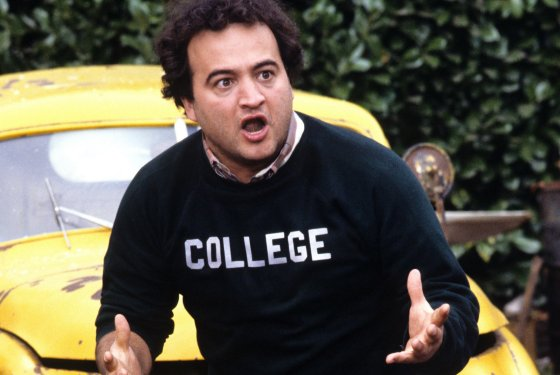
\includegraphics[max height = 0.3\textheight]{Images/belushicollege.jpg}
    }{}

    Please mute yourselves!
    \end{center}

    \ifthenelse{\equal{\thisSectionName}{Bonus}}
    {
        Get ready for some \emph{devilishly} hard questions!
        \vspace*{1em}
        % 
\includegraphics[max width=0.5\textwidth,
        %    max height=0.4\textheight]{Images/devil.jpg}
    }{}

    \vfill
  \end{frame}
}

\AtBeginSubsection[]{
  \begin{frame}
    \vfill
    \centering
    \begin{beamercolorbox}[sep=8pt,center,shadow=true,rounded=true]{title}
    \usebeamerfont{title}\insertsectionhead\par%
    \usebeamerfont{subtitle}\insertsubsectionhead\par%
    \end{beamercolorbox}
    \ifthenelse{\equal{\subsecname}{Answers}} {
        \begin{center}
        Unmute yourselves!
        \end{center}
    }
    \vfill
  \end{frame}
}
\begin{document}

\title{Welcome to Quarantine Trivia VIII!\vspace{-0.5in}}
\date{}

\begin{frame}
\titlepage{}
\begin{center}

\includegraphics[max width=0.9\textwidth,
    max height=0.4\textheight]{Images/triviatitleframelogo.png}
\end{center}
\end{frame}

\begingroup{}
\begin{frame}[t]{}
Regarding last week's beignet vs. zeppole discussion, we are always willing to
acknowledge our mistakes.  We realize now that our question should have included a
typical presentation of the pastry in question.

Beignets are typically presented in this fashion:
\pause{}
\begin{center}
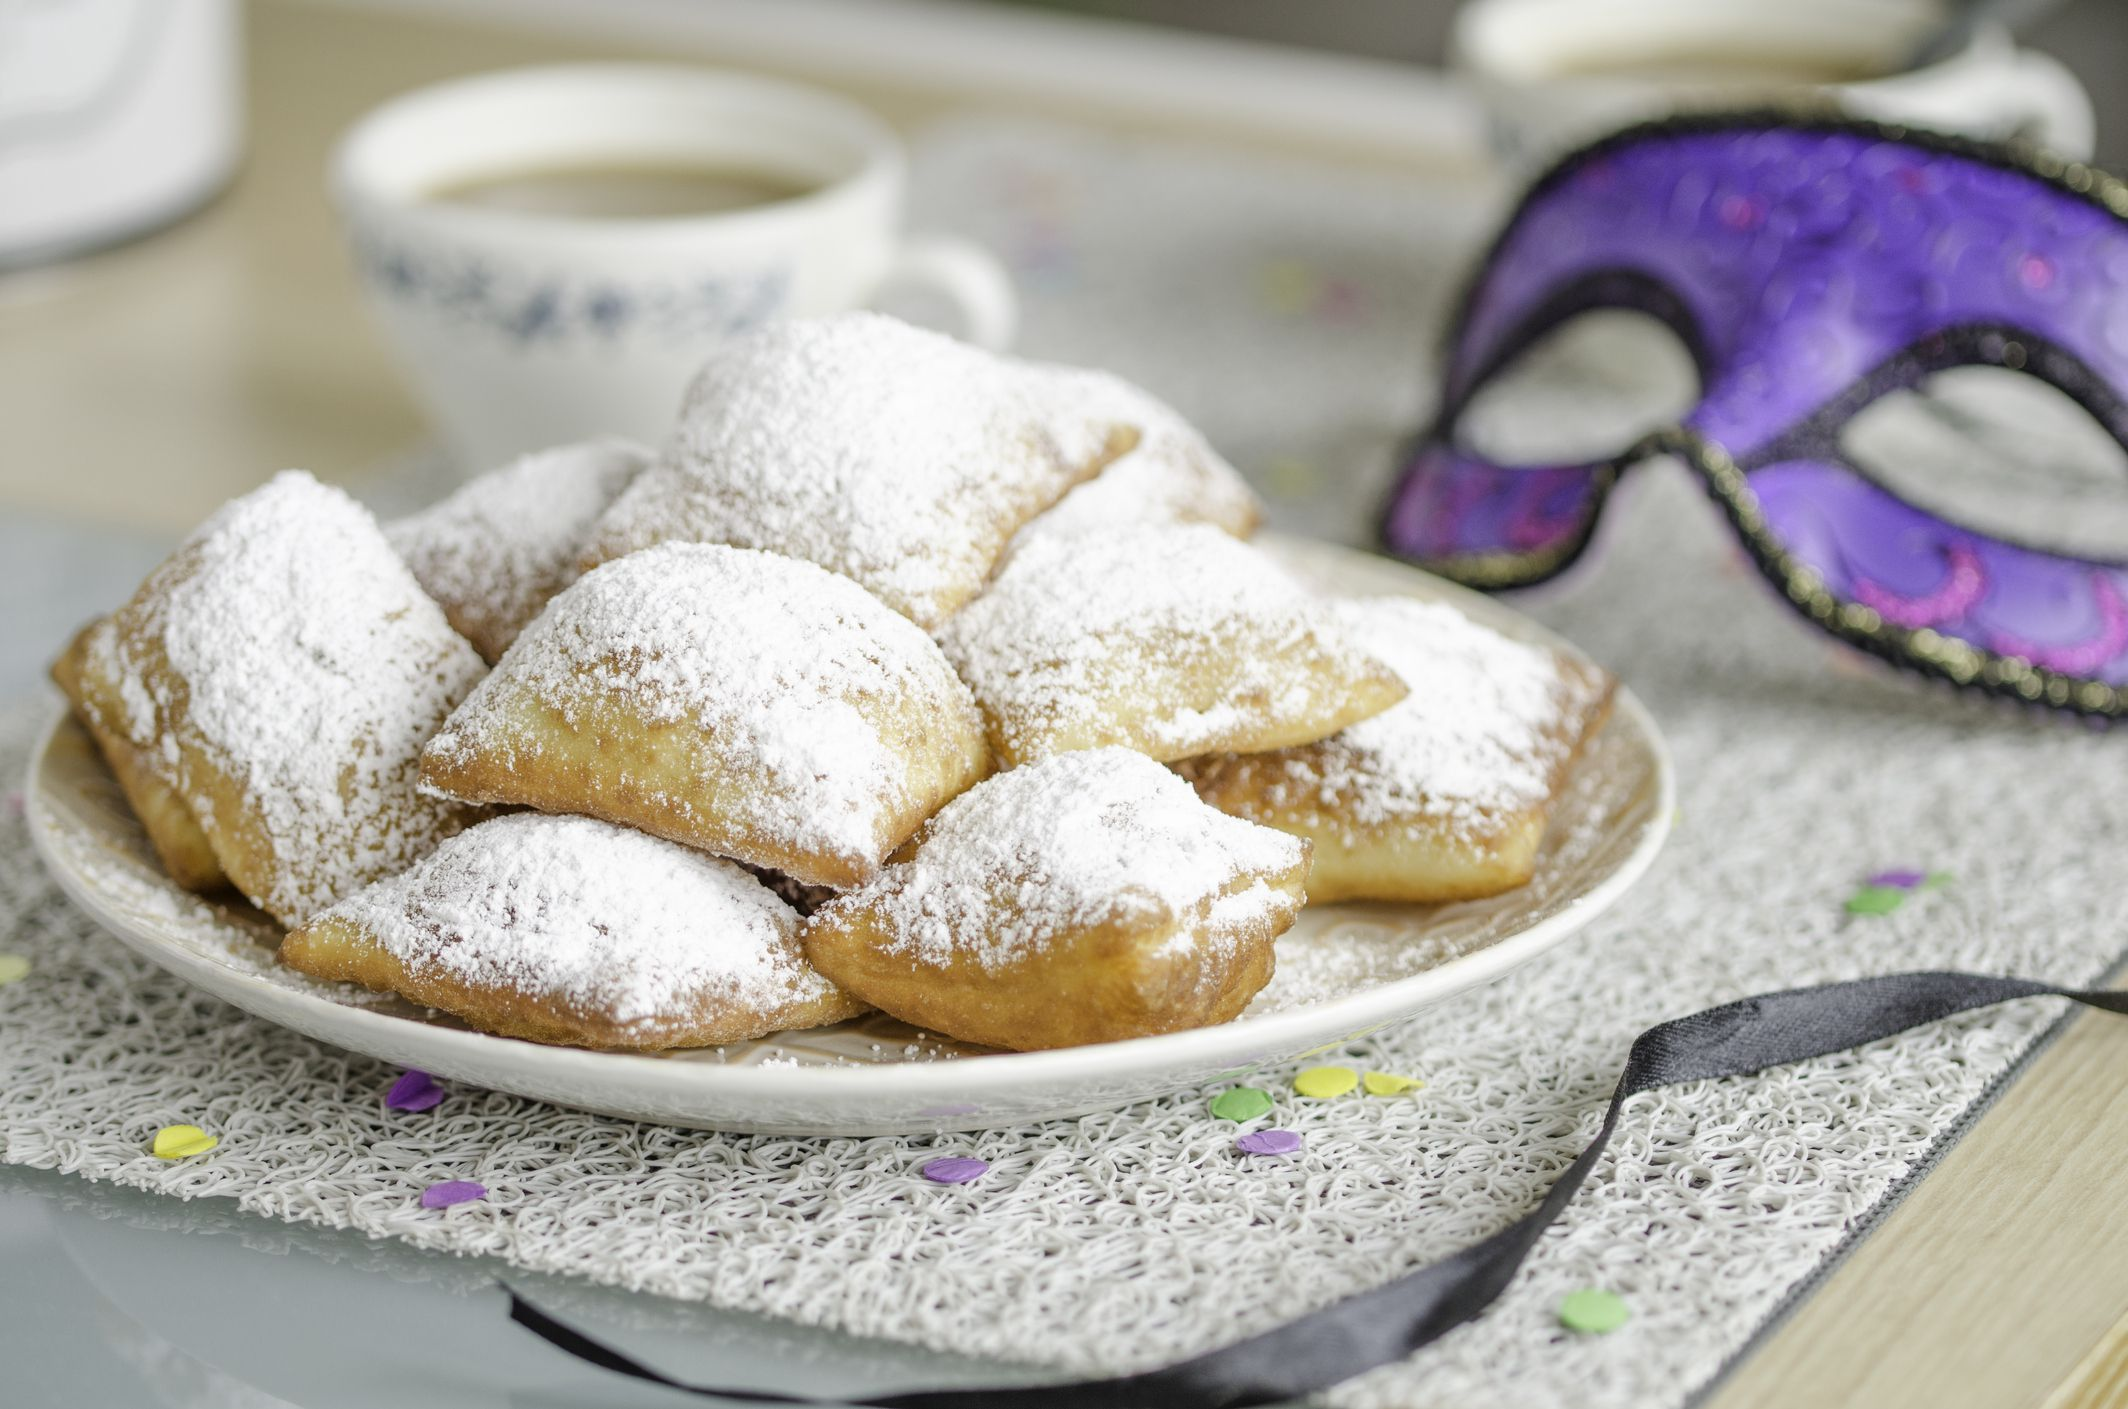
\includegraphics[max width=0.9\textwidth,
    max height=0.4\textheight]{Images/beignet.jpg}
\end{center}
\end{frame}
\begin{frame}[t]{}
Zeppole, on the other hand, are typically presented like this:
\pause{}
\begin{center}
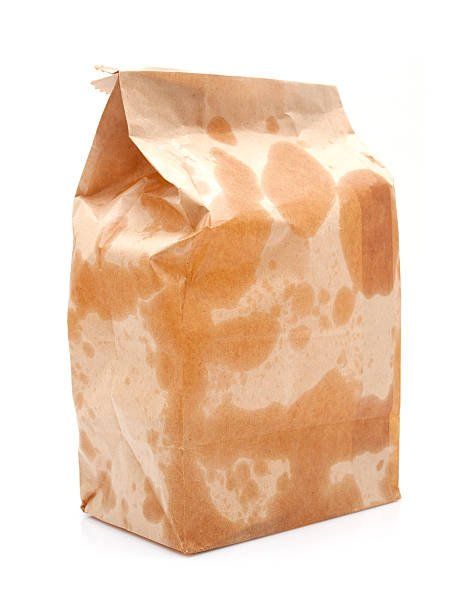
\includegraphics[max width=0.9\textwidth,
    max height=0.4\textheight]{Images/zeppole.jpg}
\end{center}
\pause{}
We apologize for any confusion we may have caused.
\end{frame}
\endgroup{}

\begingroup{}
\begin{frame}[t]{Categories}
This week, you'll be answering questions in the following categories:
\begin{enumerate}
\item Colleges and Universities
\item Horse Racing
\item The Constitution
\item It happened in 2010
\item Under the Sea
\item Myths and Legends
\item Mexico, Our Friendly Neighbor to the South
\item Famous Buildings
\item Nobel Prize Winners
\item The Beatles
\end{enumerate}
\end{frame}
\endgroup{}

\begingroup{}
\begin{frame}
\vfill{}
\begin{beamercolorbox}[sep=8pt,center,shadow=true,rounded=true]{title}
\usebeamerfont{title}Good luck everyone! And have fun!
\end{beamercolorbox}
\vfill{}
\end{frame}
\endgroup{}
\def\thisSectionName{Colleges and Universities}
\section{Round 1}
\subsection*{Q1}
\begin{frame}[t]{Round 1 --- Colleges and Universities --- \mbox{Question 1}}
\vspace{-0.5em}
\begin{block}{Question}
What was the original name of Columbia University?
\end{block}
\end{frame}
\subsection*{Q2}
\begin{frame}[t]{Round 1 --- Colleges and Universities --- \mbox{Question 2}}
\vspace{-0.5em}
\begin{block}{Question}
What college is generally  thought to be the birthplace of college football? 
\end{block}
\end{frame}
\subsection*{Q3}
\begin{frame}[t]{Round 1 --- Colleges and Universities --- \mbox{Question 3}}
\vspace{-0.5em}
\begin{block}{Question}
Which college is the second-oldest college in the U.\@S.\@?
\end{block}
\end{frame}
\subsection*{Q4}
\begin{frame}[t]{Round 1 --- Colleges and Universities --- \mbox{Question 4}}
\vspace{-0.5em}
\begin{block}{Question}
Which U.\@S.\@ college was the first to grant a degree to a woman?
\end{block}
\end{frame}
\subsection*{Q5}
\begin{frame}[t]{Round 1 --- Colleges and Universities --- \mbox{Question 5}}
\vspace{-0.5em}
\begin{block}{Question}
Which U.\@S.\@ university  has a 400-member Squirrel Club, the sole activity of which is to feed squirrels?
\end{block}
\end{frame}
\subsection*{Q6}
\begin{frame}[t]{Round 1 --- Colleges and Universities --- \mbox{Question 6}}
\vspace{-0.5em}
\begin{block}{Question}
Pres. Obama got his undergraduate degree at Columbia, but he transferred there from another college. From which college did he transfer?
\end{block}
\end{frame}
\subsection*{Q7}
\begin{frame}[t]{Round 1 --- Colleges and Universities --- \mbox{Question 7}}
\vspace{-0.5em}
\begin{block}{Question}
What college has won the most NCAA college basketball championships?
\end{block}
\end{frame}
\subsection*{Q8}
\begin{frame}[t]{Round 1 --- Colleges and Universities --- \mbox{Question 8}}
\vspace{-0.5em}
\begin{block}{Question}
What was the name of the student who led the 1964--1965 Free Speech Movement at Berkeley?
\end{block}
\end{frame}
\subsection*{Q9}
\begin{frame}[t]{Round 1 --- Colleges and Universities --- \mbox{Question 9}}
\vspace{-0.5em}
\begin{block}{Question}
Which University was founded by Thomas Jefferson?
\end{block}
\end{frame}
\subsection*{Q10}
\begin{frame}[t]{Round 1 --- Colleges and Universities --- \mbox{Question 10}}
\vspace{-0.5em}
\begin{block}{Question}
Fill in the blank in this college fight song: ``I'm a Ramblin' Wreck from Georgia Tech and a hell of a[n] \textunderscore{}\textunderscore{}\textunderscore{}\textunderscore{}\textunderscore{}.'' 
\end{block}
\end{frame}
\subsection{Answers}
\begin{frame}[t]{Round 1 --- Colleges and Universities --- \mbox{Answer 1}}
\vspace{-0.5em}
\begin{block}{Question}
What was the original name of Columbia University?
\end{block}

\visible<2->{
    \begin{columns}[T,totalwidth=\linewidth]
    \begin{column}{0.32\linewidth}
    \begin{block}{Answer}
    King's College
    \end{block}
    \end{column}
    \begin{column}{0.65\linewidth}
    \begin{center}
    
\includegraphics[max width=0.95\textwidth,
        max height=0.58000\textheight]{{Images/columbia}.png}
    \end{center}
    \end{column}
    \end{columns}
}
\end{frame}
\begin{frame}[t]{Round 1 --- Colleges and Universities --- \mbox{Answer 2}}
\vspace{-0.5em}
\begin{block}{Question}
What college is generally  thought to be the birthplace of college football? 
\end{block}

\visible<2->{
    \begin{columns}[T,totalwidth=\linewidth]
    \begin{column}{0.32\linewidth}
    \begin{block}{Answer}
    Rutgers
    \end{block}
    \end{column}
    \begin{column}{0.65\linewidth}
    \begin{center}
    
\includegraphics[max width=0.95\textwidth,
        max height=0.54000\textheight]{{Images/rutgers}.jpg}
    \end{center}
    \end{column}
    \end{columns}
}
\end{frame}
\begin{frame}[t]{Round 1 --- Colleges and Universities --- \mbox{Answer 3}}
\vspace{-0.5em}
\begin{block}{Question}
Which college is the second-oldest college in the U.\@S.\@?
\end{block}

\visible<2->{
    \begin{columns}[T,totalwidth=\linewidth]
    \begin{column}{0.32\linewidth}
    \begin{block}{Answer}
    William and Mary
    \end{block}
    \end{column}
    \begin{column}{0.65\linewidth}
    \begin{center}
    
\includegraphics[max width=0.95\textwidth,
        max height=0.54000\textheight]{{Images/wmc}.jpg}
    \end{center}
    \end{column}
    \end{columns}
}
\end{frame}
\begin{frame}[t]{Round 1 --- Colleges and Universities --- \mbox{Answer 4}}
\vspace{-0.5em}
\begin{block}{Question}
Which U.\@S.\@ college was the first to grant a degree to a woman?
\end{block}

\visible<2->{
    \begin{columns}[T,totalwidth=\linewidth]
    \begin{column}{0.32\linewidth}
    \begin{block}{Answer}
    Oberlin, in 1841
    \end{block}
    \end{column}
    \begin{column}{0.65\linewidth}
    \begin{center}
    
\includegraphics[max width=0.95\textwidth,
        max height=0.54000\textheight]{{Images/oberlin}.png}
    \end{center}
    \end{column}
    \end{columns}
}
\end{frame}
\begin{frame}[t]{Round 1 --- Colleges and Universities --- \mbox{Answer 5}}
\vspace{-0.5em}
\begin{block}{Question}
Which U.\@S.\@ university  has a 400-member Squirrel Club, the sole activity of which is to feed squirrels?
\end{block}

\visible<2->{
    \begin{columns}[T,totalwidth=\linewidth]
    \begin{column}{0.32\linewidth}
    \begin{block}{Answer}
    University of Michigan
    \end{block}
    \end{column}
    \begin{column}{0.65\linewidth}
    \begin{center}
    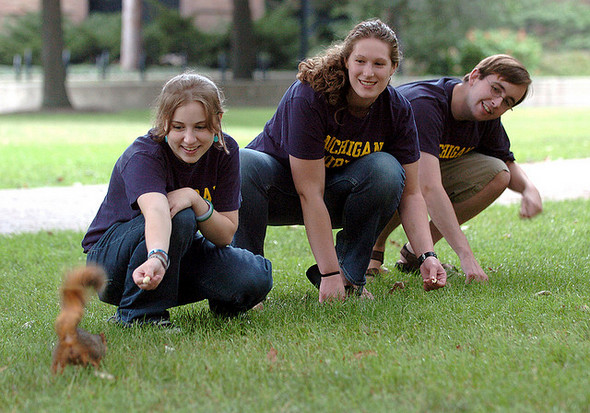
\includegraphics[max width=0.95\textwidth,
        max height=0.50000\textheight]{{Images/michigan}.jpg}
    \end{center}
    \end{column}
    \end{columns}
}
\end{frame}
\begin{frame}[t]{Round 1 --- Colleges and Universities --- \mbox{Answer 6}}
\vspace{-0.5em}
\begin{block}{Question}
Pres. Obama got his undergraduate degree at Columbia, but he transferred there from another college. From which college did he transfer?
\end{block}

\visible<2->{
    \begin{columns}[T,totalwidth=\linewidth]
    \begin{column}{0.32\linewidth}
    \begin{block}{Answer}
    Occidental College
    \end{block}
    \end{column}
    \begin{column}{0.65\linewidth}
    \begin{center}
    
\includegraphics[max width=0.95\textwidth,
        max height=0.50000\textheight]{{Images/occy}.png}
    \end{center}
    \end{column}
    \end{columns}
}
\end{frame}
\begin{frame}[t]{Round 1 --- Colleges and Universities --- \mbox{Answer 7}}
\vspace{-0.5em}
\begin{block}{Question}
What college has won the most NCAA college basketball championships?
\end{block}

\visible<2->{
    \begin{columns}[T,totalwidth=\linewidth]
    \begin{column}{0.32\linewidth}
    \begin{block}{Answer}
    UCLA, with 11
    \end{block}
    \end{column}
    \begin{column}{0.65\linewidth}
    \begin{center}
    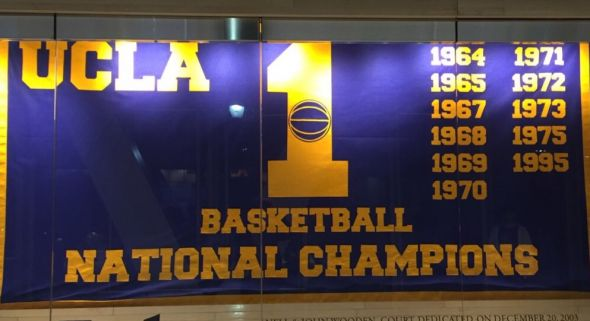
\includegraphics[max width=0.95\textwidth,
        max height=0.54000\textheight]{{Images/ucla}.jpg}
    \end{center}
    \end{column}
    \end{columns}
}
\end{frame}
\begin{frame}[t]{Round 1 --- Colleges and Universities --- \mbox{Answer 8}}
\vspace{-0.5em}
\begin{block}{Question}
What was the name of the student who led the 1964--1965 Free Speech Movement at Berkeley?
\end{block}

\visible<2->{
    \begin{columns}[T,totalwidth=\linewidth]
    \begin{column}{0.32\linewidth}
    \begin{block}{Answer}
    Mario Savio
    \end{block}
    \end{column}
    \begin{column}{0.65\linewidth}
    \begin{center}
    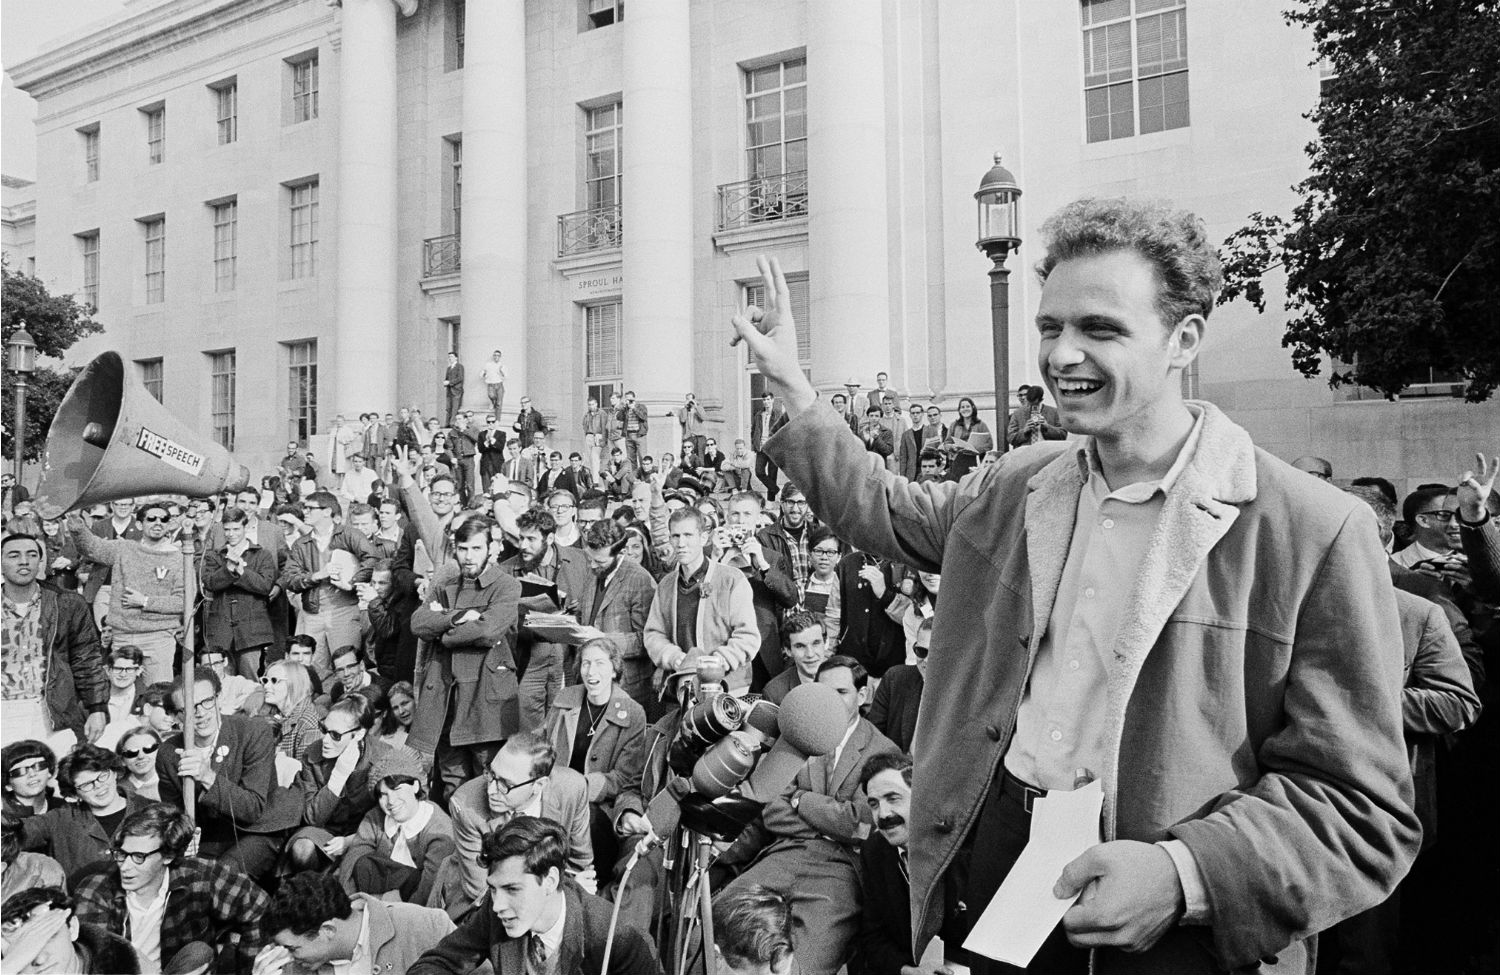
\includegraphics[max width=0.95\textwidth,
        max height=0.54000\textheight]{{Images/salvio}.jpg}
    \end{center}
    \end{column}
    \end{columns}
}
\end{frame}
\begin{frame}[t]{Round 1 --- Colleges and Universities --- \mbox{Answer 9}}
\vspace{-0.5em}
\begin{block}{Question}
Which University was founded by Thomas Jefferson?
\end{block}

\visible<2->{
    \begin{columns}[T,totalwidth=\linewidth]
    \begin{column}{0.32\linewidth}
    \begin{block}{Answer}
    The University of Virginia
    \end{block}
    \end{column}
    \begin{column}{0.65\linewidth}
    \begin{center}
    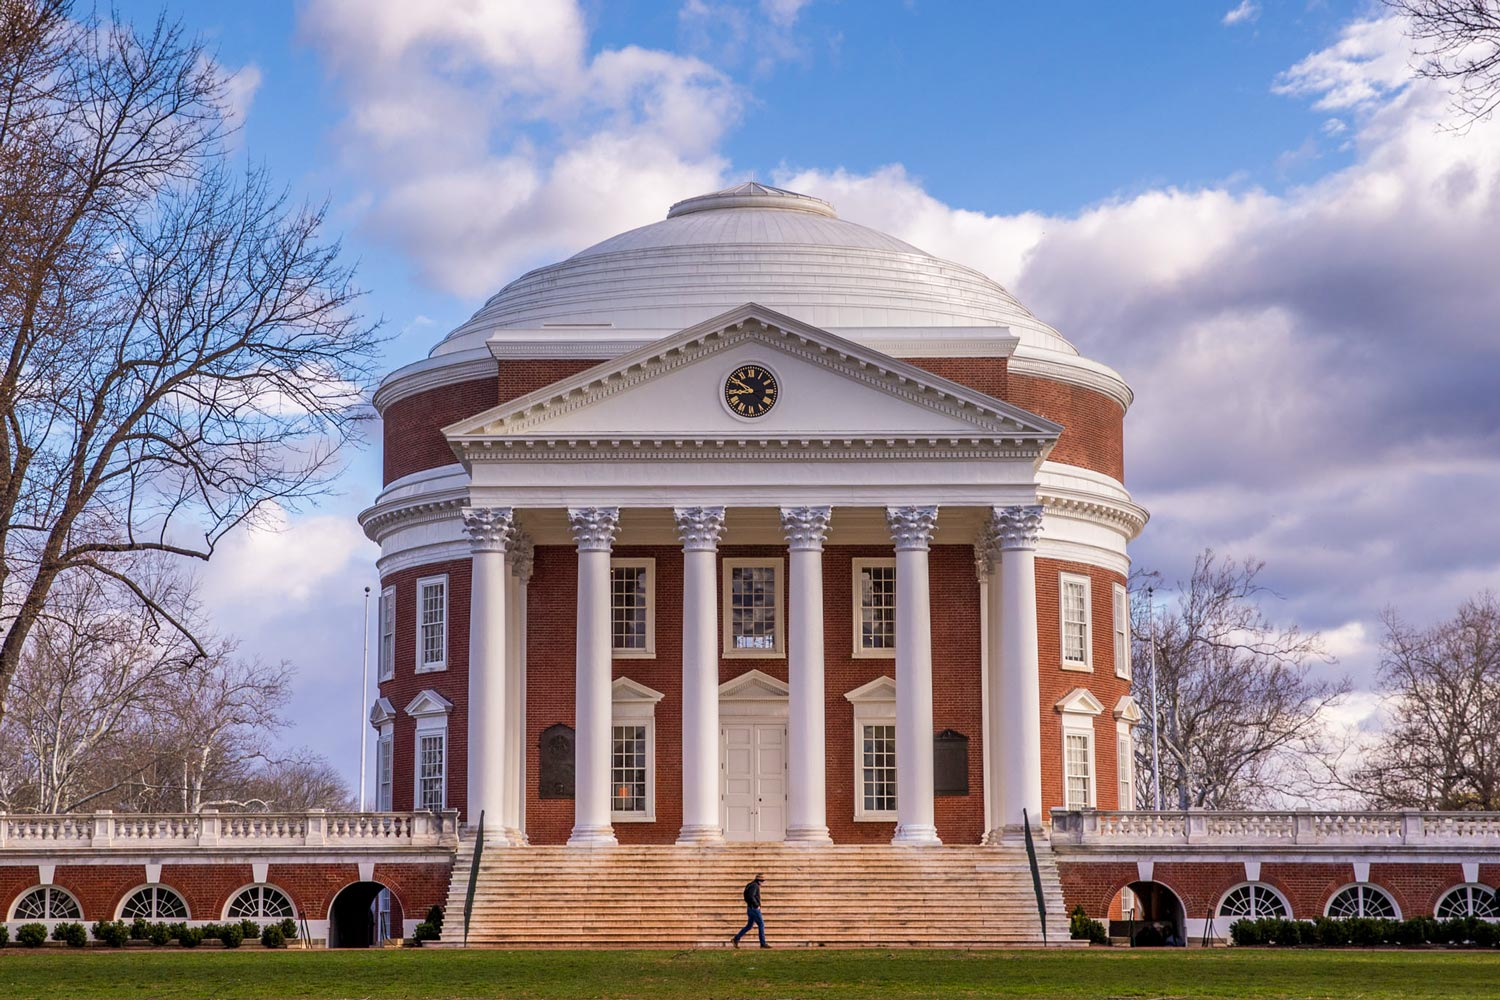
\includegraphics[max width=0.95\textwidth,
        max height=0.58000\textheight]{{Images/uva}.jpg}
    \end{center}
    \end{column}
    \end{columns}
}
\end{frame}
\begin{frame}[t]{Round 1 --- Colleges and Universities --- \mbox{Answer 10}}
\vspace{-0.5em}
\begin{block}{Question}
Fill in the blank in this college fight song: ``I'm a Ramblin' Wreck from Georgia Tech and a hell of a[n] \textunderscore{}\textunderscore{}\textunderscore{}\textunderscore{}\textunderscore{}.'' 
\end{block}

\visible<2->{
    \begin{columns}[T,totalwidth=\linewidth]
    \begin{column}{0.32\linewidth}
    \begin{block}{Answer}
    Engineer
    \end{block}
    \end{column}
    \begin{column}{0.65\linewidth}
    \begin{center}
    
\includegraphics[max width=0.95\textwidth,
        max height=0.46000\textheight]{{Images/gatech}.jpeg}
    \end{center}
    \end{column}
    \end{columns}
}
\end{frame}
\def\thisSectionName{Horse Racing}
\section{Round 2}
\subsection*{Q1}
\begin{frame}[t]{Round 2 --- Horse Racing --- \mbox{Question 1}}
\vspace{-0.5em}
\begin{block}{Question}
Potoooooooo was a famous 18\textsuperscript{th} century racehorse who won 30 races and defeated many of the best horses of his day. His name has the same pronunciation as a common English word. How is his name pronounced?
\end{block}
\end{frame}
\subsection*{Q2}
\begin{frame}[t]{Round 2 --- Horse Racing --- \mbox{Question 2}}
\vspace{-0.5em}
\begin{block}{Question}
Which horse most recently won the Triple Crowns?
\end{block}
\end{frame}
\subsection*{Q3}
\begin{frame}[t]{Round 2 --- Horse Racing --- \mbox{Question 3}}
\vspace{-0.5em}
\begin{block}{Question}
What is the name of the first horse to win the Triple Crown?
\end{block}
\end{frame}
\subsection*{Q4}
\begin{frame}[t]{Round 2 --- Horse Racing --- \mbox{Question 4}}
\vspace{-0.5em}
\begin{block}{Question}
What are the names of the races that make up the Triple Crown? We need all three.
\end{block}
\end{frame}
\subsection*{Q5}
\begin{frame}[t]{Round 2 --- Horse Racing --- \mbox{Question 5}}
\vspace{-0.5em}
\begin{block}{Question}
Which sire is responsible for the most horses in the U.\@S.\@ Racing Hall of Fame?
\end{block}
\end{frame}
\subsection*{Q6}
\begin{frame}[t]{Round 2 --- Horse Racing --- \mbox{Question 6}}
\vspace{-0.5em}
\begin{block}{Question}
Who is the only female jockey to win a Triple Crown race?
\end{block}
\end{frame}
\subsection*{Q7}
\begin{frame}[t]{Round 2 --- Horse Racing --- \mbox{Question 7}}
\vspace{-0.5em}
\begin{block}{Question}
What is the name of the horse farm in Lexington Kentucky that has produced more winners of Triple Crown races than any other horse farm?
\end{block}
\end{frame}
\subsection*{Q8}
\begin{frame}[t]{Round 2 --- Horse Racing --- \mbox{Question 8}}
\vspace{-0.5em}
\begin{block}{Question}
What is the name of the underdog horse who surprisingly beat Triple Crown winner War Admiral in a race held on November 1, 1938?
\end{block}
\end{frame}
\subsection*{Q9}
\begin{frame}[t]{Round 2 --- Horse Racing --- \mbox{Question 9}}
\vspace{-0.5em}
\begin{block}{Question}
What is the name of the musician who had a novelty hit about a horse race with a racing announcer saying lines like, ``Cabbage is second by a head'', ``Mother-In-Law nagging in the rear'', and ``Banana is coming up through the bunch?''
\end{block}
\end{frame}
\subsection*{Q10}
\begin{frame}[t]{Round 2 --- Horse Racing --- \mbox{Question 10}}
\vspace{-0.5em}
\begin{block}{Question}
What is the name of the first filly to run in all the Triple Crown races?

\end{block}
\end{frame}
\subsection{Answers}
\begin{frame}[t]{Round 2 --- Horse Racing --- \mbox{Answer 1}}
\vspace{-0.5em}
\begin{block}{Question}
Potoooooooo was a famous 18\textsuperscript{th} century racehorse who won 30 races and defeated many of the best horses of his day. His name has the same pronunciation as a common English word. How is his name pronounced?
\end{block}

\visible<2->{
    \begin{columns}[T,totalwidth=\linewidth]
    \begin{column}{0.32\linewidth}
    \begin{block}{Answer}
    Potatoes (Pot 8 Os)
    \end{block}
    \end{column}
    \begin{column}{0.65\linewidth}
    \begin{center}
    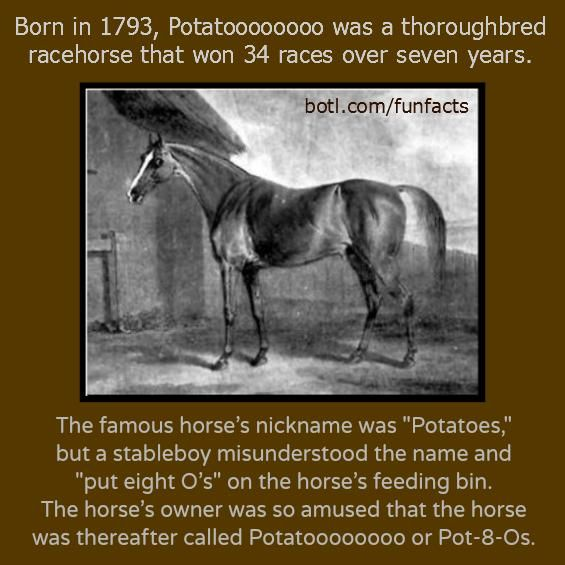
\includegraphics[max width=0.95\textwidth,
        max height=0.42000\textheight]{{Images/potoooooooos}.jpg}
    \end{center}
    \end{column}
    \end{columns}
}
\end{frame}
\begin{frame}[t]{Round 2 --- Horse Racing --- \mbox{Answer 2}}
\vspace{-0.5em}
\begin{block}{Question}
Which horse most recently won the Triple Crowns?
\end{block}

\visible<2->{
    \begin{columns}[T,totalwidth=\linewidth]
    \begin{column}{0.32\linewidth}
    \begin{block}{Answer}
    Justify, 2018
    \end{block}
    \end{column}
    \begin{column}{0.65\linewidth}
    \begin{center}
    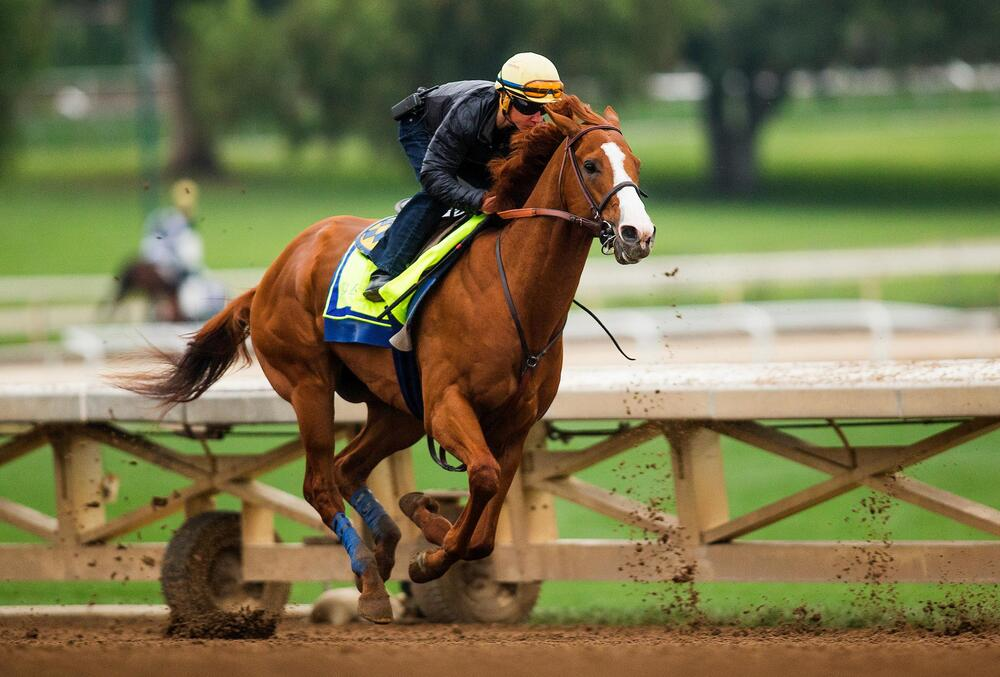
\includegraphics[max width=0.95\textwidth,
        max height=0.58000\textheight]{{Images/justify}.jpg}
    \end{center}
    \end{column}
    \end{columns}
}
\end{frame}
\begin{frame}[t]{Round 2 --- Horse Racing --- \mbox{Answer 3}}
\vspace{-0.5em}
\begin{block}{Question}
What is the name of the first horse to win the Triple Crown?
\end{block}

\visible<2->{
    \begin{columns}[T,totalwidth=\linewidth]
    \begin{column}{0.32\linewidth}
    \begin{block}{Answer}
    Sir Barton, 1919
    \end{block}
    \end{column}
    \begin{column}{0.65\linewidth}
    \begin{center}
    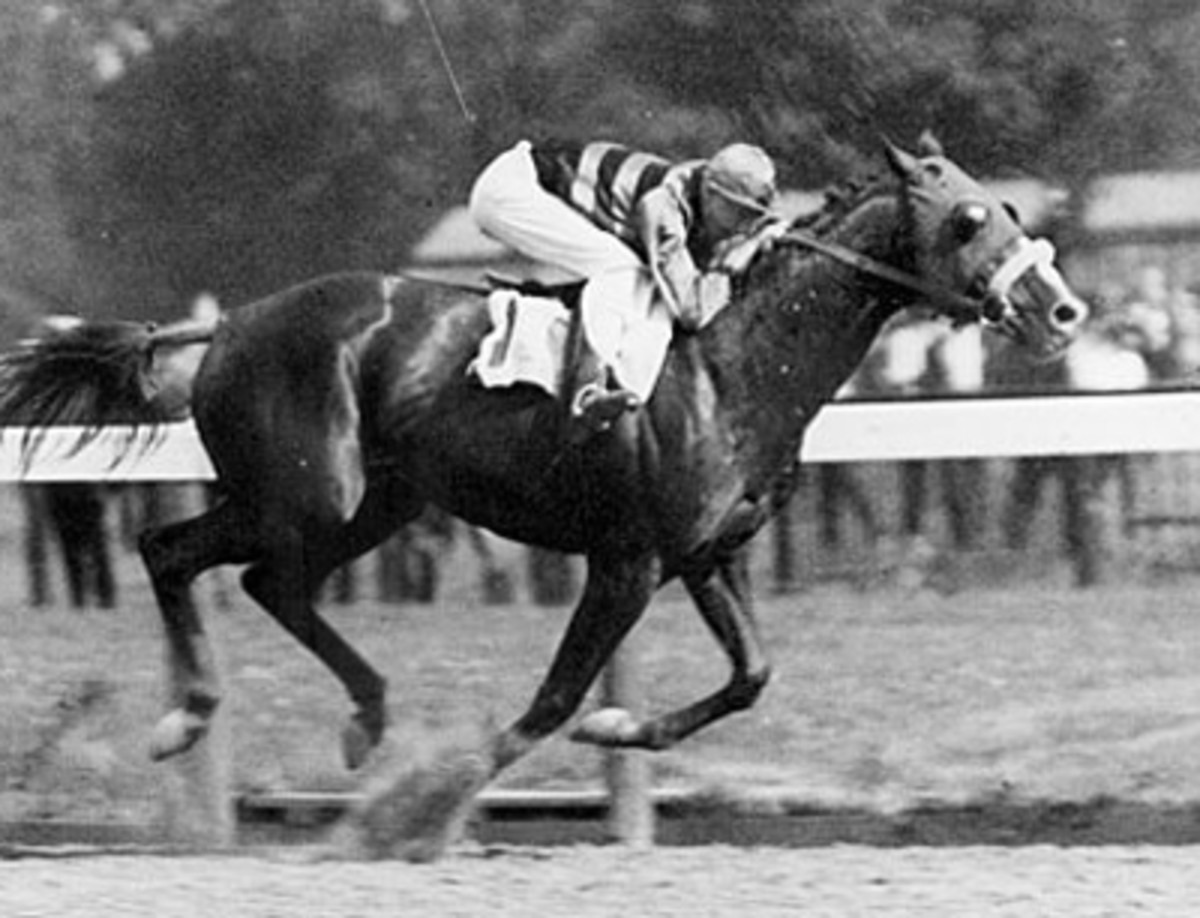
\includegraphics[max width=0.95\textwidth,
        max height=0.54000\textheight]{{Images/sirbarton}.jpg}
    \end{center}
    \end{column}
    \end{columns}
}
\end{frame}
\begin{frame}[t]{Round 2 --- Horse Racing --- \mbox{Answer 4}}
\vspace{-0.5em}
\begin{block}{Question}
What are the names of the races that make up the Triple Crown? We need all three.
\end{block}

\visible<2->{
    \begin{columns}[T,totalwidth=\linewidth]
    \begin{column}{0.32\linewidth}
    \begin{block}{Answer}
    The Kentucky Derby, the Preakness Stakes and the Belmont Stakes (Preakness and Belmont without ``Stakes'' is fine)
    \end{block}
    \end{column}
    \begin{column}{0.65\linewidth}
    \begin{center}
    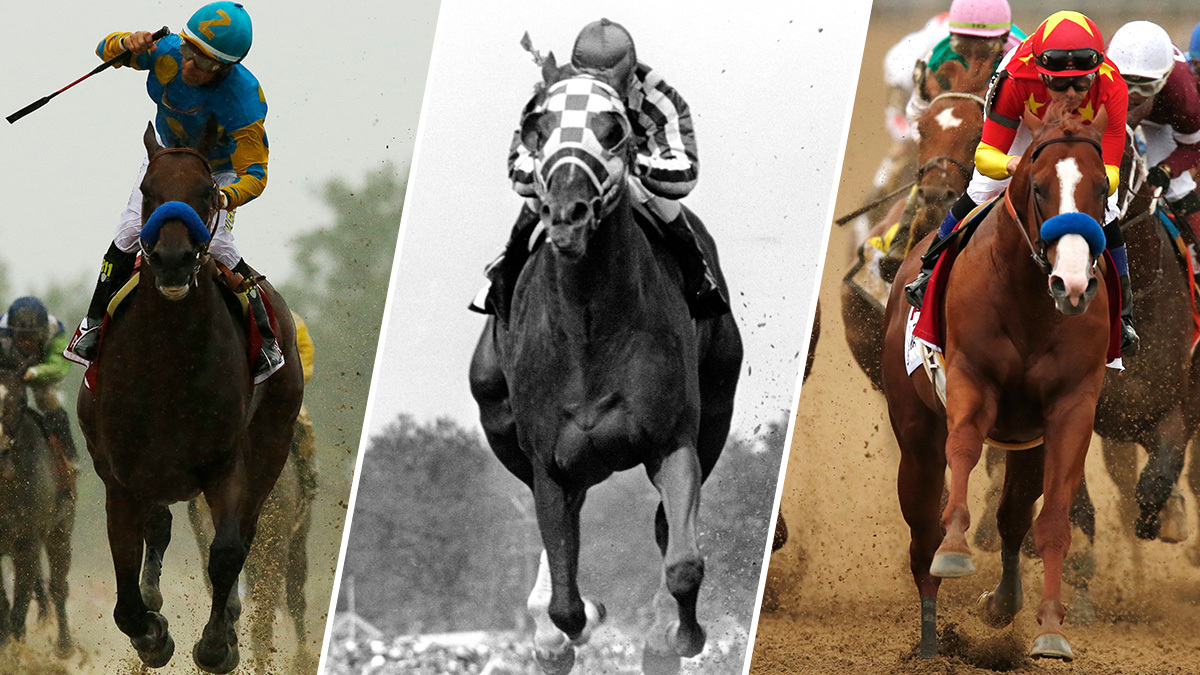
\includegraphics[max width=0.95\textwidth,
        max height=0.54000\textheight]{{Images/triplecrown}.jpg}
    \end{center}
    \end{column}
    \end{columns}
}
\end{frame}
\begin{frame}[t]{Round 2 --- Horse Racing --- \mbox{Answer 5}}
\vspace{-0.5em}
\begin{block}{Question}
Which sire is responsible for the most horses in the U.\@S.\@ Racing Hall of Fame?
\end{block}

\visible<2->{
    \begin{columns}[T,totalwidth=\linewidth]
    \begin{column}{0.32\linewidth}
    \begin{block}{Answer}
    Bull Lea
    \end{block}
    \end{column}
    \begin{column}{0.65\linewidth}
    \begin{center}
    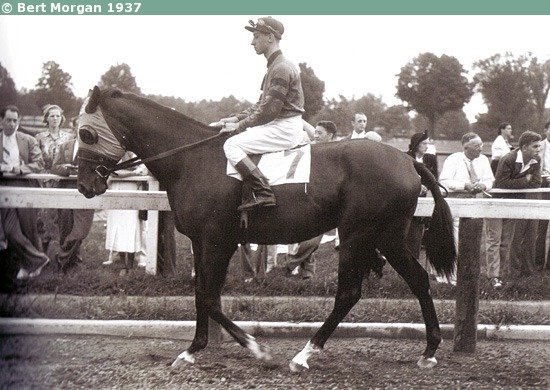
\includegraphics[max width=0.95\textwidth,
        max height=0.54000\textheight]{{Images/bulllea}.jpg}
    \end{center}
    \end{column}
    \end{columns}
}
\end{frame}
\begin{frame}[t]{Round 2 --- Horse Racing --- \mbox{Answer 6}}
\vspace{-0.5em}
\begin{block}{Question}
Who is the only female jockey to win a Triple Crown race?
\end{block}

\visible<2->{
    \begin{columns}[T,totalwidth=\linewidth]
    \begin{column}{0.32\linewidth}
    \begin{block}{Answer}
    Julie Krone, who won the 1993 Belmont Stakes on Colonial Affair


    \end{block}
    \end{column}
    \begin{column}{0.65\linewidth}
    \begin{center}
    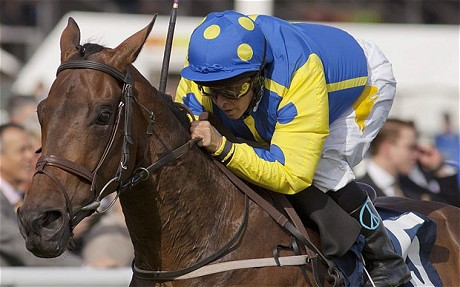
\includegraphics[max width=0.95\textwidth,
        max height=0.54000\textheight]{{Images/krone}.jpg}
    \end{center}
    \end{column}
    \end{columns}
}
\end{frame}
\begin{frame}[t]{Round 2 --- Horse Racing --- \mbox{Answer 7}}
\vspace{-0.5em}
\begin{block}{Question}
What is the name of the horse farm in Lexington Kentucky that has produced more winners of Triple Crown races than any other horse farm?
\end{block}

\visible<2->{
    \begin{columns}[T,totalwidth=\linewidth]
    \begin{column}{0.32\linewidth}
    \begin{block}{Answer}
    Calumet Farm, which has produced 18 winners of Triple Crown races
    \end{block}
    \end{column}
    \begin{column}{0.65\linewidth}
    \begin{center}
    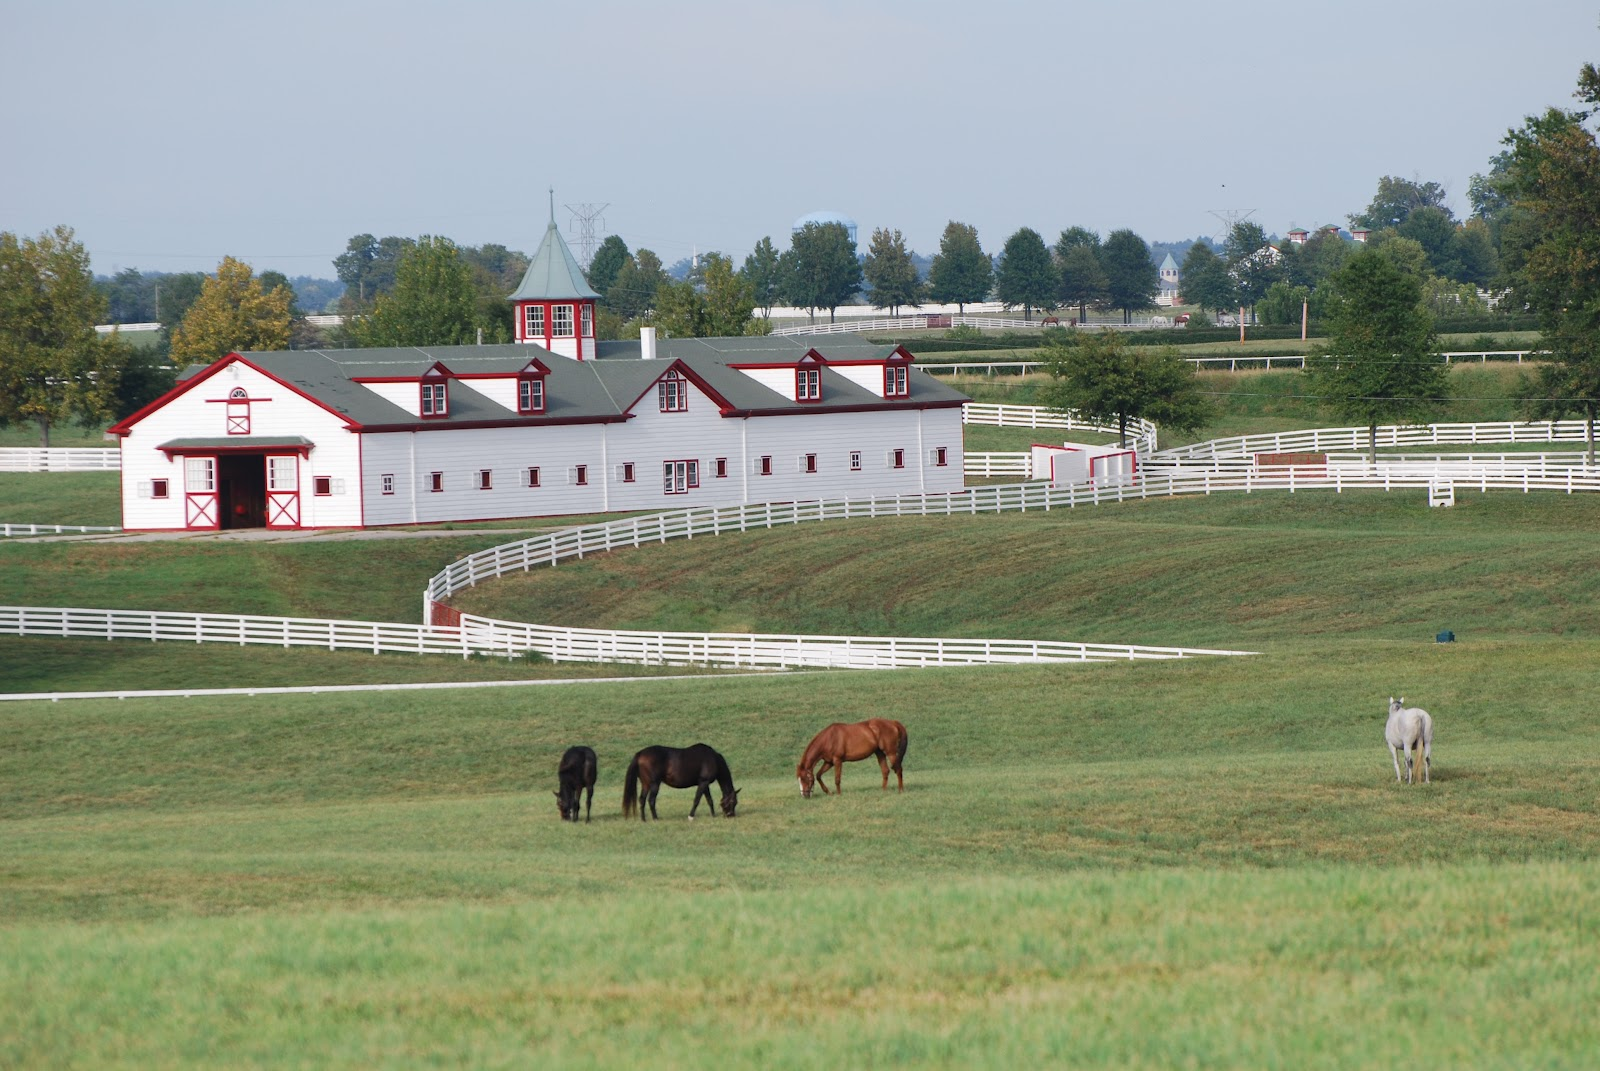
\includegraphics[max width=0.95\textwidth,
        max height=0.50000\textheight]{{Images/calumet}.JPG}
    \end{center}
    \end{column}
    \end{columns}
}
\end{frame}
\begin{frame}[t]{Round 2 --- Horse Racing --- \mbox{Answer 8}}
\vspace{-0.5em}
\begin{block}{Question}
What is the name of the underdog horse who surprisingly beat Triple Crown winner War Admiral in a race held on November 1, 1938?
\end{block}

\visible<2->{
    \begin{columns}[T,totalwidth=\linewidth]
    \begin{column}{0.32\linewidth}
    \begin{block}{Answer}
    Seabiscuit
    \end{block}
    \end{column}
    \begin{column}{0.65\linewidth}
    \begin{center}
    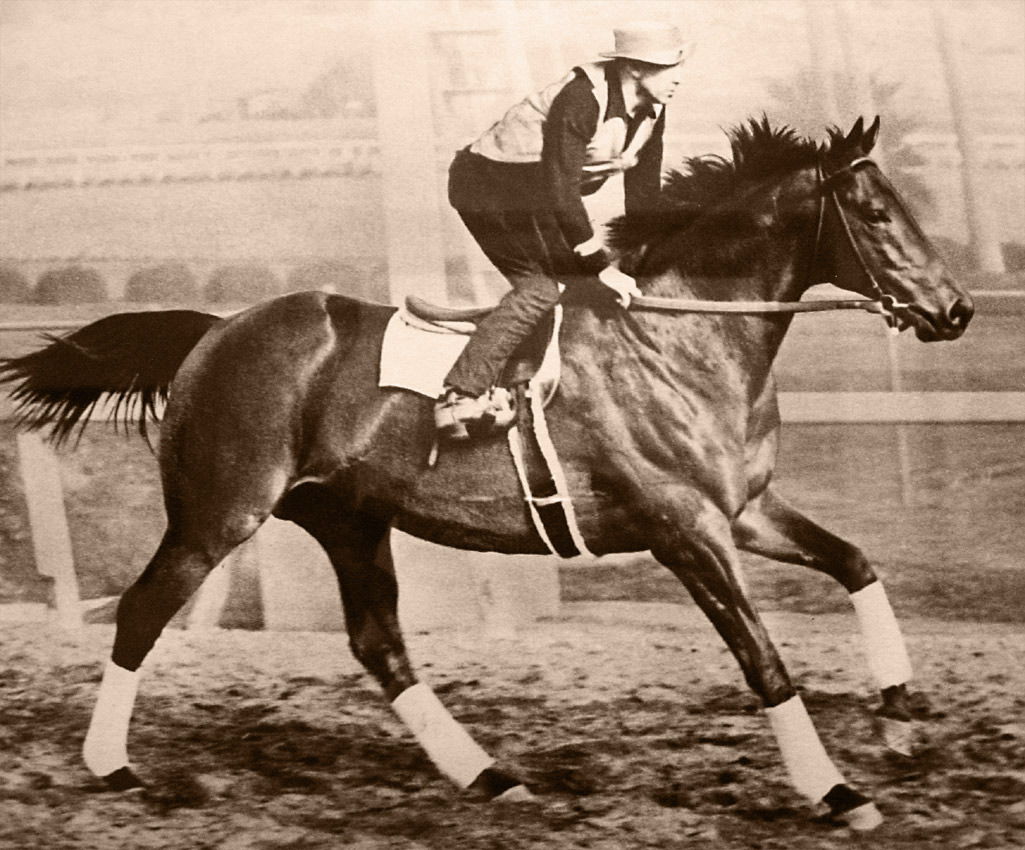
\includegraphics[max width=0.95\textwidth,
        max height=0.50000\textheight]{{Images/seabiscuit}.jpg}
    \end{center}
    \end{column}
    \end{columns}
}
\end{frame}
\begin{frame}[t]{Round 2 --- Horse Racing --- \mbox{Answer 9}}
\vspace{-0.5em}
\begin{block}{Question}
What is the name of the musician who had a novelty hit about a horse race with a racing announcer saying lines like, ``Cabbage is second by a head'', ``Mother-In-Law nagging in the rear'', and ``Banana is coming up through the bunch?''
\end{block}

\visible<2->{
    \begin{columns}[T,totalwidth=\linewidth]
    \begin{column}{0.32\linewidth}
    \begin{block}{Answer}
    Spike Jones
    \end{block}
    \end{column}
    \begin{column}{0.65\linewidth}
    \begin{center}
    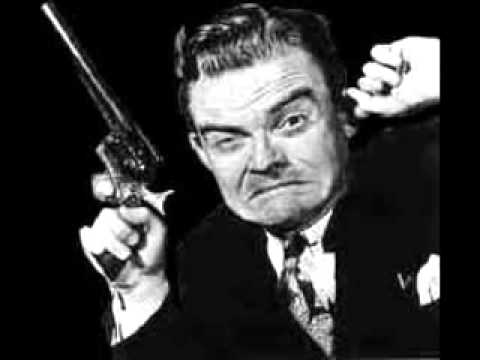
\includegraphics[max width=0.95\textwidth,
        max height=0.42000\textheight]{{Images/spikejones}.jpg}
    \end{center}
    \end{column}
    \end{columns}
}
\end{frame}
\begin{frame}[t]{Round 2 --- Horse Racing --- \mbox{Answer 10}}
\vspace{-0.5em}
\begin{block}{Question}
What is the name of the first filly to run in all the Triple Crown races?

\end{block}

\visible<2->{
    \begin{columns}[T,totalwidth=\linewidth]
    \begin{column}{0.32\linewidth}
    \begin{block}{Answer}
    Genuine Risk. In 1980, she won the Kentucky Derby and placed in both the Preakness and Belmont Stakes.
    \end{block}
    \end{column}
    \begin{column}{0.65\linewidth}
    \begin{center}
    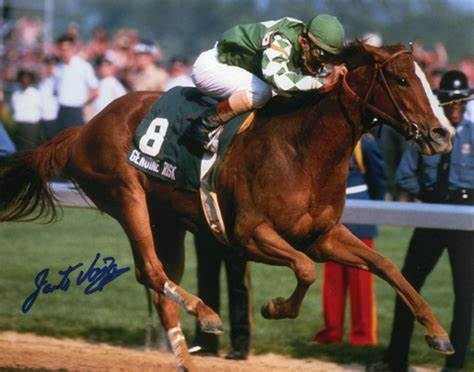
\includegraphics[max width=0.95\textwidth,
        max height=0.54000\textheight]{{Images/genuinerisk}.jpeg}
    \end{center}
    \end{column}
    \end{columns}
}
\end{frame}
\def\thisSectionName{The Constitution}
\section{Round 3}
\subsection*{Q1}
\begin{frame}[t]{Round 3 --- The Constitution --- \mbox{Question 1}}
\vspace{-0.5em}
\begin{block}{Question}
Fill in the blank in the first sentence of the Constitution: ``We the People of the United States, in Order to form a more perfect \textunderscore{}\textunderscore{}\textunderscore{}\textunderscore{}\textunderscore{}, establish \ldots{}''
\end{block}
\end{frame}
\subsection*{Q2}
\begin{frame}[t]{Round 3 --- The Constitution --- \mbox{Question 2}}
\vspace{-0.5em}
\begin{block}{Question}
Which amendment gave rise to the income tax?
\end{block}
\end{frame}
\subsection*{Q3}
\begin{frame}[t]{Round 3 --- The Constitution --- \mbox{Question 3}}
\vspace{-0.5em}
\begin{block}{Question}
During the Constitutional Convention, what was the name of the compromise that the large and small states of the Union made in which they agreed that the U.\@S.\@ would have a bicameral legislature? (It has multiple names; any one will do.)
\end{block}
\end{frame}
\subsection*{Q4}
\begin{frame}[t]{Round 3 --- The Constitution --- \mbox{Question 4}}
\vspace{-0.5em}
\begin{block}{Question}
The Constitution describes the powers and limitations of the three branches of government. Which branch does it describe first, in Article I\@?
\end{block}
\end{frame}
\subsection*{Q5}
\begin{frame}[t]{Round 3 --- The Constitution --- \mbox{Question 5}}
\vspace{-0.5em}
\begin{block}{Question}
Of the thirteen original states, which one was the last to ratify the Constitution?
\end{block}
\end{frame}
\subsection*{Q6}
\begin{frame}[t]{Round 3 --- The Constitution --- \mbox{Question 6}}
\vspace{-0.5em}
\begin{block}{Question}
The final article of the Constitution, Article VII, only contains a single sentence, which dictates that how many of the original thirteen states must sign the Constitution in order for it to become law?
\end{block}
\end{frame}
\subsection*{Q7}
\begin{frame}[t]{Round 3 --- The Constitution --- \mbox{Question 7}}
\vspace{-0.5em}
\begin{block}{Question}
In which city did the Constitutional Convention take place?
\end{block}
\end{frame}
\subsection*{Q8}
\begin{frame}[t]{Round 3 --- The Constitution --- \mbox{Question 8}}
\vspace{-0.5em}
\begin{block}{Question}
What is the name of the system set out in the Constitution in which power was to be divided between federal and state governments?
\end{block}
\end{frame}
\subsection*{Q9}
\begin{frame}[t]{Round 3 --- The Constitution --- \mbox{Question 9}}
\vspace{-0.5em}
\begin{block}{Question}
Which amendment had the most time pass being submitted and being ratified?
\end{block}
\end{frame}
\subsection*{Q10}
\begin{frame}[t]{Round 3 --- The Constitution --- \mbox{Question 10}}
\vspace{-0.5em}
\begin{block}{Question}
We all know that the Constitution says the president ``shall \ldots{} have attained to the Age of thirty five Years'', but it also says the president shall have been ``a Resident within the United States'' for how many years?
\end{block}
\end{frame}
\subsection{Answers}
\begin{frame}[t]{Round 3 --- The Constitution --- \mbox{Answer 1}}
\vspace{-0.5em}
\begin{block}{Question}
Fill in the blank in the first sentence of the Constitution: ``We the People of the United States, in Order to form a more perfect \textunderscore{}\textunderscore{}\textunderscore{}\textunderscore{}\textunderscore{}, establish \ldots{}''
\end{block}

\visible<2->{
    \begin{columns}[T,totalwidth=\linewidth]
    \begin{column}{0.32\linewidth}
    \begin{block}{Answer}
    Union
    \end{block}
    \end{column}
    \begin{column}{0.65\linewidth}
    \begin{center}
    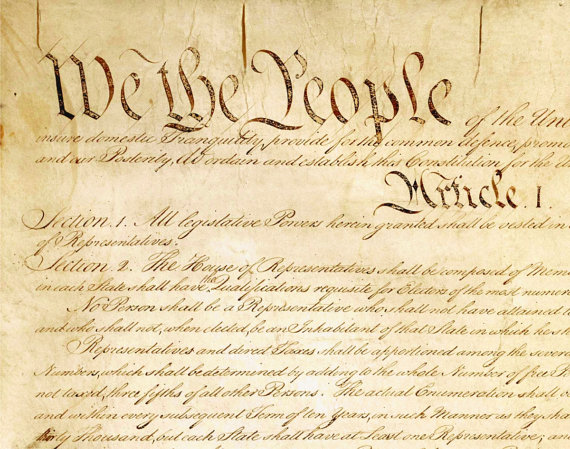
\includegraphics[max width=0.95\textwidth,
        max height=0.42000\textheight]{{Images/preamble}.jpg}
    \end{center}
    \end{column}
    \end{columns}
}
\end{frame}
\begin{frame}[t]{Round 3 --- The Constitution --- \mbox{Answer 2}}
\vspace{-0.5em}
\begin{block}{Question}
Which amendment gave rise to the income tax?
\end{block}

\visible<2->{
    \begin{columns}[T,totalwidth=\linewidth]
    \begin{column}{0.32\linewidth}
    \begin{block}{Answer}
    The 16\textsuperscript{th} Amendment
    \end{block}
    \end{column}
    \begin{column}{0.65\linewidth}
    \begin{center}
    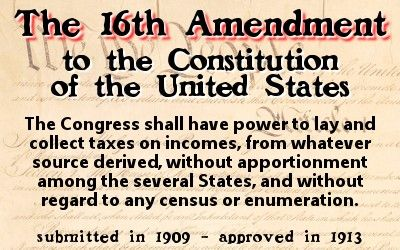
\includegraphics[max width=0.95\textwidth,
        max height=0.58000\textheight]{{Images/incometax}.jpg}
    \end{center}
    \end{column}
    \end{columns}
}
\end{frame}
\begin{frame}[t]{Round 3 --- The Constitution --- \mbox{Answer 3}}
\vspace{-0.5em}
\begin{block}{Question}
During the Constitutional Convention, what was the name of the compromise that the large and small states of the Union made in which they agreed that the U.\@S.\@ would have a bicameral legislature? (It has multiple names; any one will do.)
\end{block}

\visible<2->{
    \begin{columns}[T,totalwidth=\linewidth]
    \begin{column}{0.32\linewidth}
    \begin{block}{Answer}
    The Great Compromise / The Connecticut Compromise / The Sherman Compromise
    \end{block}
    \end{column}
    \begin{column}{0.65\linewidth}
    \begin{center}
    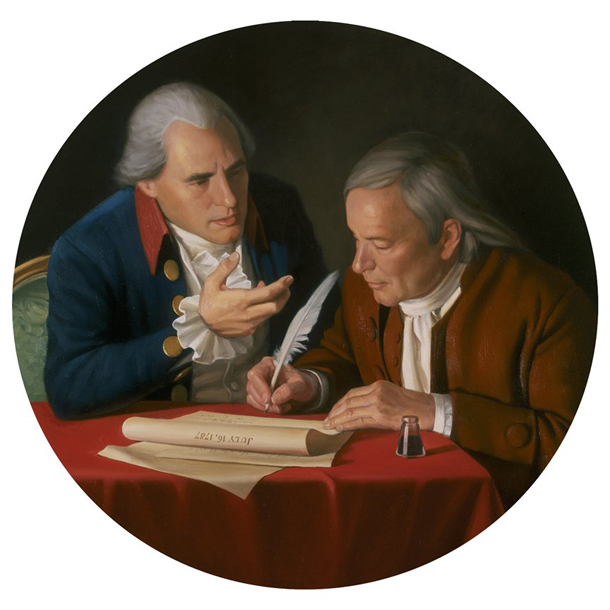
\includegraphics[max width=0.95\textwidth,
        max height=0.42000\textheight]{{Images/connecticutcompromise}.jpg}
    \end{center}
    \end{column}
    \end{columns}
}
\end{frame}
\begin{frame}[t]{Round 3 --- The Constitution --- \mbox{Answer 4}}
\vspace{-0.5em}
\begin{block}{Question}
The Constitution describes the powers and limitations of the three branches of government. Which branch does it describe first, in Article I\@?
\end{block}

\visible<2->{
    \begin{columns}[T,totalwidth=\linewidth]
    \begin{column}{0.32\linewidth}
    \begin{block}{Answer}
    The legislative branch / Congress
    \end{block}
    \end{column}
    \begin{column}{0.65\linewidth}
    \begin{center}
    
\includegraphics[max width=0.95\textwidth,
        max height=0.50000\textheight]{{Images/congress}.png}
    \end{center}
    \end{column}
    \end{columns}
}
\end{frame}
\begin{frame}[t]{Round 3 --- The Constitution --- \mbox{Answer 5}}
\vspace{-0.5em}
\begin{block}{Question}
Of the thirteen original states, which one was the last to ratify the Constitution?
\end{block}

\visible<2->{
    \begin{columns}[T,totalwidth=\linewidth]
    \begin{column}{0.32\linewidth}
    \begin{block}{Answer}
    Rhode Island
    \end{block}
    \end{column}
    \begin{column}{0.65\linewidth}
    \begin{center}
    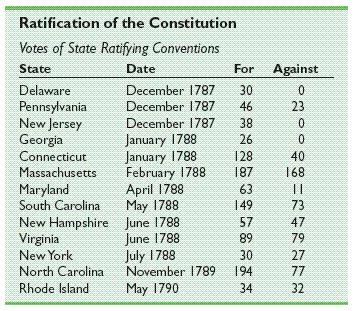
\includegraphics[max width=0.95\textwidth,
        max height=0.54000\textheight]{{Images/ratification}.JPG}
    \end{center}
    \end{column}
    \end{columns}
}
\end{frame}
\begin{frame}[t]{Round 3 --- The Constitution --- \mbox{Answer 6}}
\vspace{-0.5em}
\begin{block}{Question}
The final article of the Constitution, Article VII, only contains a single sentence, which dictates that how many of the original thirteen states must sign the Constitution in order for it to become law?
\end{block}

\visible<2->{
    \begin{columns}[T,totalwidth=\linewidth]
    \begin{column}{0.32\linewidth}
    \begin{block}{Answer}
    Nine
    \end{block}
    \end{column}
    \begin{column}{0.65\linewidth}
    \begin{center}
    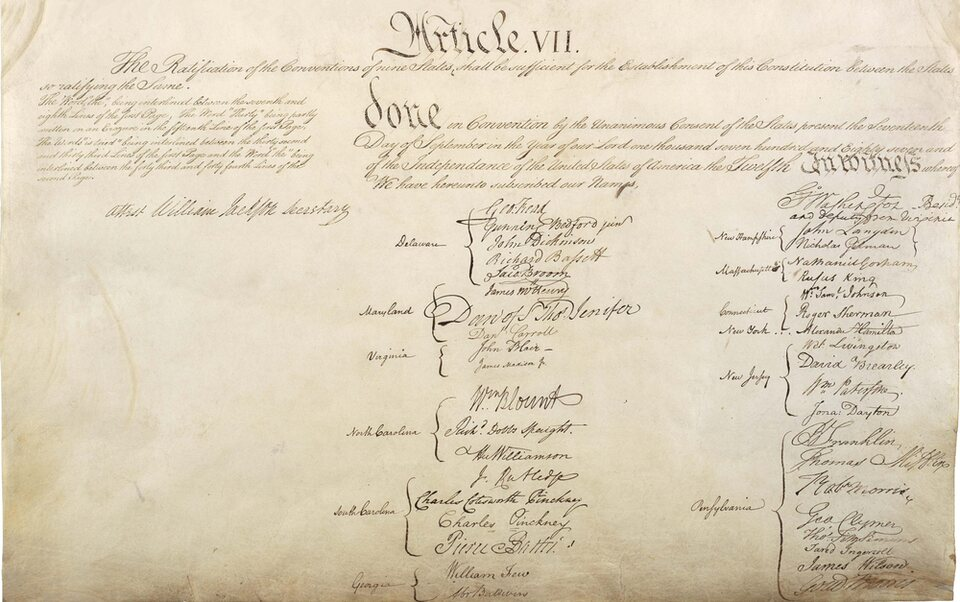
\includegraphics[max width=0.95\textwidth,
        max height=0.42000\textheight]{{Images/articlevii}.jpg}
    \end{center}
    \end{column}
    \end{columns}
}
\end{frame}
\begin{frame}[t]{Round 3 --- The Constitution --- \mbox{Answer 7}}
\vspace{-0.5em}
\begin{block}{Question}
In which city did the Constitutional Convention take place?
\end{block}

\visible<2->{
    \begin{columns}[T,totalwidth=\linewidth]
    \begin{column}{0.32\linewidth}
    \begin{block}{Answer}
    Philadelphia
    \end{block}
    \end{column}
    \begin{column}{0.65\linewidth}
    \begin{center}
    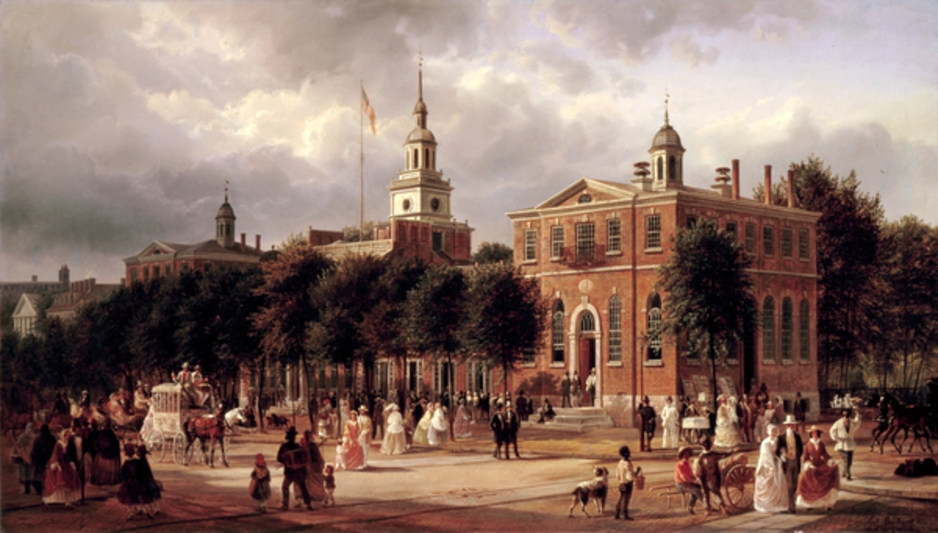
\includegraphics[max width=0.95\textwidth,
        max height=0.54000\textheight]{{Images/philly}.jpg}
    \end{center}
    \end{column}
    \end{columns}
}
\end{frame}
\begin{frame}[t]{Round 3 --- The Constitution --- \mbox{Answer 8}}
\vspace{-0.5em}
\begin{block}{Question}
What is the name of the system set out in the Constitution in which power was to be divided between federal and state governments?
\end{block}

\visible<2->{
    \begin{columns}[T,totalwidth=\linewidth]
    \begin{column}{0.32\linewidth}
    \begin{block}{Answer}
    Federalism
    \end{block}
    \end{column}
    \begin{column}{0.65\linewidth}
    \begin{center}
    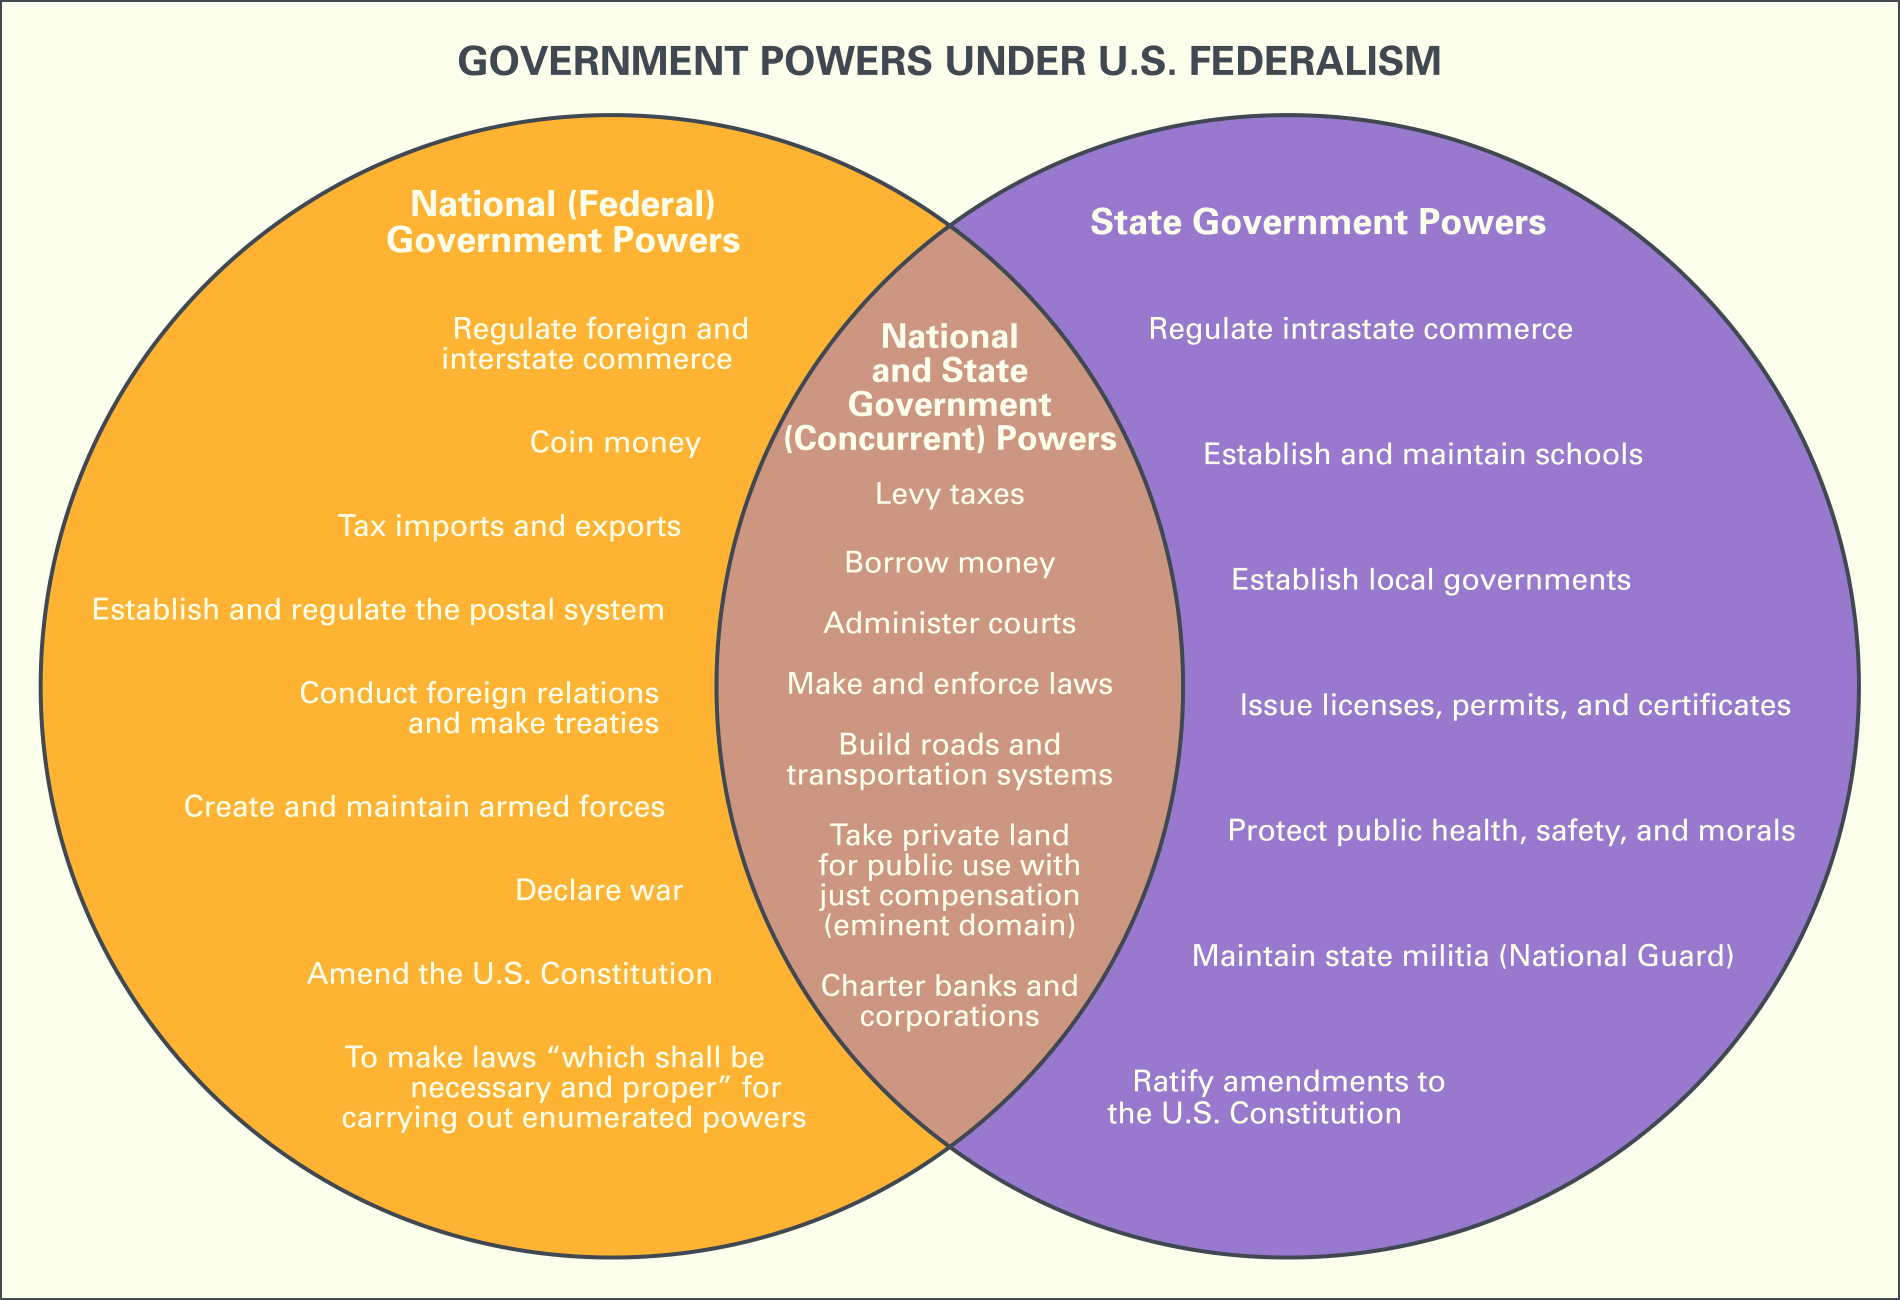
\includegraphics[max width=0.95\textwidth,
        max height=0.50000\textheight]{{Images/federalism}.jpg}
    \end{center}
    \end{column}
    \end{columns}
}
\end{frame}
\begin{frame}[t]{Round 3 --- The Constitution --- \mbox{Answer 9}}
\vspace{-0.5em}
\begin{block}{Question}
Which amendment had the most time pass being submitted and being ratified?
\end{block}

\visible<2->{
    \begin{columns}[T,totalwidth=\linewidth]
    \begin{column}{0.32\linewidth}
    \begin{block}{Answer}
    The 27\textsuperscript{th} Amendment. (Submitted Sept. 25, 1789, ratified May 5, 1992 --- nearly 203 years).
    \end{block}
    \end{column}
    \begin{column}{0.65\linewidth}
    \begin{center}
    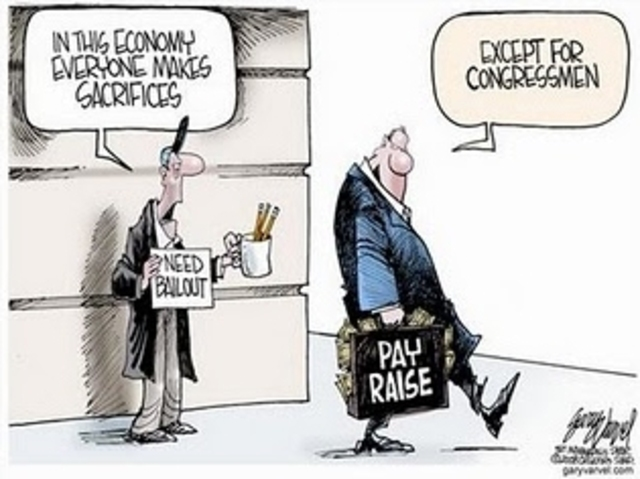
\includegraphics[max width=0.95\textwidth,
        max height=0.54000\textheight]{{Images/amendment27}.jpg}
    \end{center}
    \end{column}
    \end{columns}
}
\end{frame}
\begin{frame}[t]{Round 3 --- The Constitution --- \mbox{Answer 10}}
\vspace{-0.5em}
\begin{block}{Question}
We all know that the Constitution says the president ``shall \ldots{} have attained to the Age of thirty five Years'', but it also says the president shall have been ``a Resident within the United States'' for how many years?
\end{block}
\visible<2->{
    \begin{block}{Answer}
    Fourteen
    \end{block}
}
\end{frame}
\def\thisSectionName{It happened in 2010}
\section{Round 4}
\subsection*{Q1}
\begin{frame}[t]{Round 4 --- It happened in 2010 --- \mbox{Question 1}}
\vspace{-0.5em}
\begin{block}{Question}
On January 12\textsuperscript{th}, which country was devastated by a massive earthquake?
\end{block}
\end{frame}
\subsection*{Q2}
\begin{frame}[t]{Round 4 --- It happened in 2010 --- \mbox{Question 2}}
\vspace{-0.5em}
\begin{block}{Question}
On February 7\textsuperscript{th}, which NFL  team won the Super Bowl?
\end{block}
\end{frame}
\subsection*{Q3}
\begin{frame}[t]{Round 4 --- It happened in 2010 --- \mbox{Question 3}}
\vspace{-0.5em}
\begin{block}{Question}
On February 12\textsuperscript{th}, the winter Olympic Games opened in which city?
\end{block}
\end{frame}
\subsection*{Q4}
\begin{frame}[t]{Round 4 --- It happened in 2010 --- \mbox{Question 4}}
\vspace{-0.5em}
\begin{block}{Question}
On April 14\textsuperscript{th}, the volcano Eyjafjallajökull began erupting. The eruption ultimately caused problems with air travel. In which country was the volcano located?
\end{block}
\end{frame}
\subsection*{Q5}
\begin{frame}[t]{Round 4 --- It happened in 2010 --- \mbox{Question 5}}
\vspace{-0.5em}
\begin{block}{Question}
What was the name of the drilling rig that exploded in the Gulf of Mexico on April 20\textsuperscript{th}?
\end{block}
\end{frame}
\subsection*{Q6}
\begin{frame}[t]{Round 4 --- It happened in 2010 --- \mbox{Question 6}}
\vspace{-0.5em}
\begin{block}{Question}
Who became British Prime Minister on May 11\textsuperscript{th}?
\end{block}
\end{frame}
\subsection*{Q7}
\begin{frame}[t]{Round 4 --- It happened in 2010 --- \mbox{Question 7}}
\vspace{-0.5em}
\begin{block}{Question}
On May 29\textsuperscript{th}, which MLB pitcher became the 20\textsuperscript{th} MLB pitcher to throw a perfect game?
\end{block}
\end{frame}
\subsection*{Q8}
\begin{frame}[t]{Round 4 --- It happened in 2010 --- \mbox{Question 8}}
\vspace{-0.5em}
\begin{block}{Question}
On July 3\textsuperscript{rd}, who won the Wimbledon Women's Championship?
\end{block}
\end{frame}
\subsection*{Q9}
\begin{frame}[t]{Round 4 --- It happened in 2010 --- \mbox{Question 9}}
\vspace{-0.5em}
\begin{block}{Question}
On November 1\textsuperscript{st}, which team won the World Series?
\end{block}
\end{frame}
\subsection*{Q10}
\begin{frame}[t]{Round 4 --- It happened in 2010 --- \mbox{Question 10}}
\vspace{-0.5em}
\begin{block}{Question}
On December 10\textsuperscript{th}, who was awarded the Nobel Peace Prize while imprisoned?
\end{block}
\end{frame}
\subsection{Answers}
\begin{frame}[t]{Round 4 --- It happened in 2010 --- \mbox{Answer 1}}
\vspace{-0.5em}
\begin{block}{Question}
On January 12\textsuperscript{th}, which country was devastated by a massive earthquake?
\end{block}

\visible<2->{
    \begin{columns}[T,totalwidth=\linewidth]
    \begin{column}{0.32\linewidth}
    \begin{block}{Answer}
    Haiti
    \end{block}
    \end{column}
    \begin{column}{0.65\linewidth}
    \begin{center}
    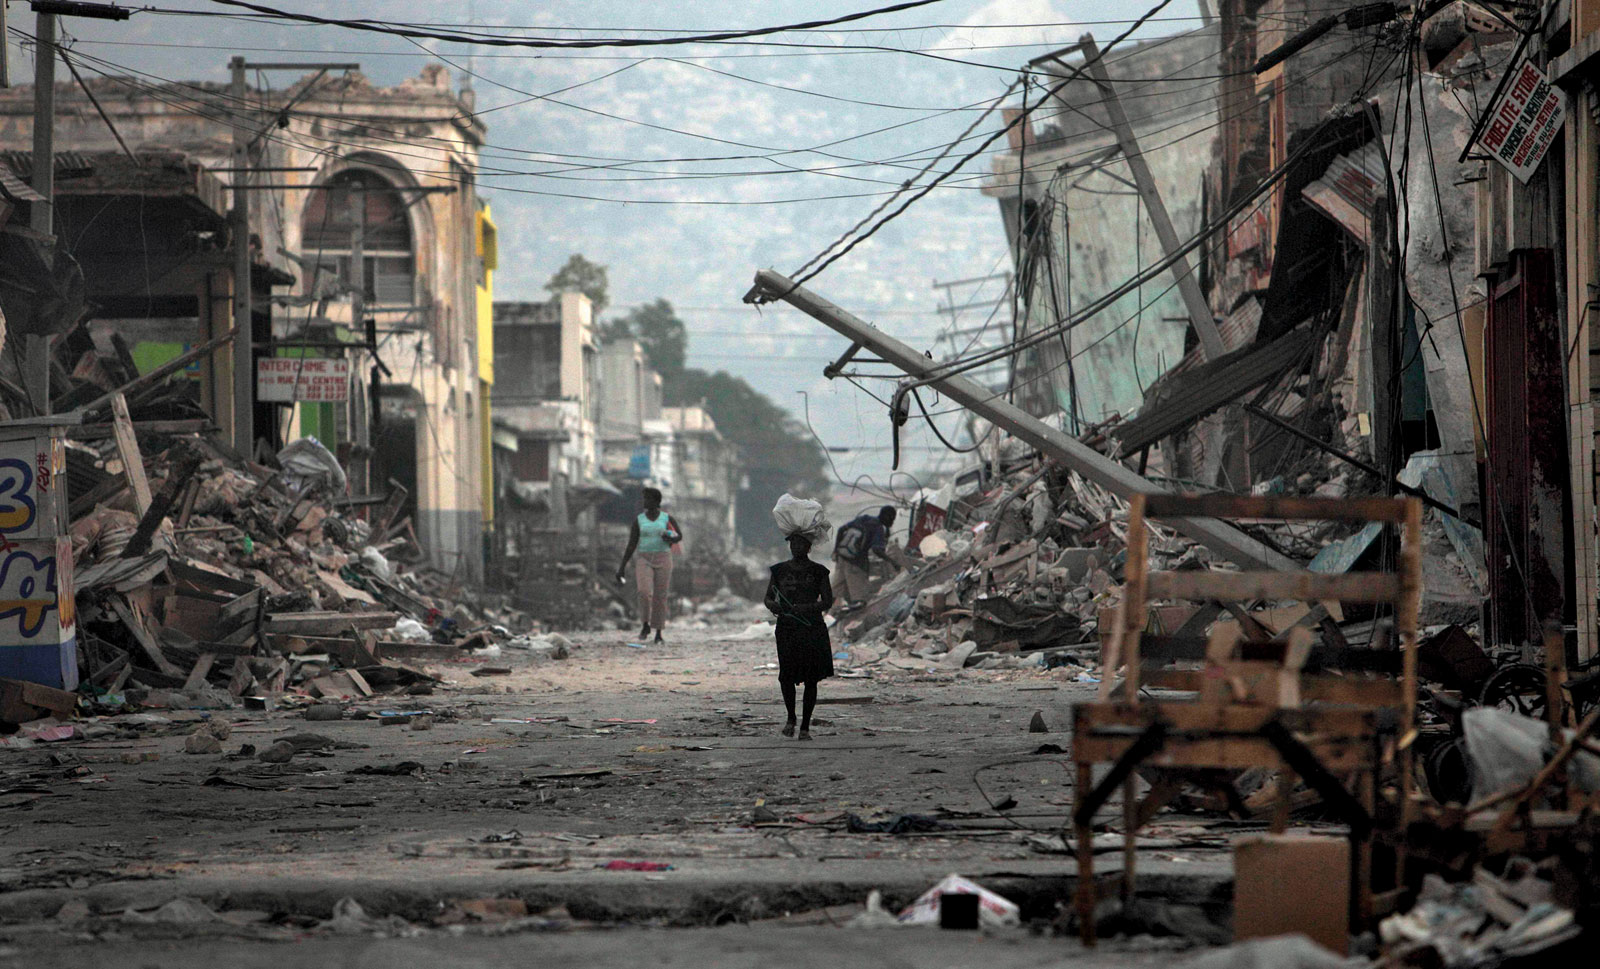
\includegraphics[max width=0.95\textwidth,
        max height=0.54000\textheight]{{Images/haiti}.jpg}
    \end{center}
    \end{column}
    \end{columns}
}
\end{frame}
\begin{frame}[t]{Round 4 --- It happened in 2010 --- \mbox{Answer 2}}
\vspace{-0.5em}
\begin{block}{Question}
On February 7\textsuperscript{th}, which NFL  team won the Super Bowl?
\end{block}

\visible<2->{
    \begin{columns}[T,totalwidth=\linewidth]
    \begin{column}{0.32\linewidth}
    \begin{block}{Answer}
    New Orleans Saints
    \end{block}
    \end{column}
    \begin{column}{0.65\linewidth}
    \begin{center}
    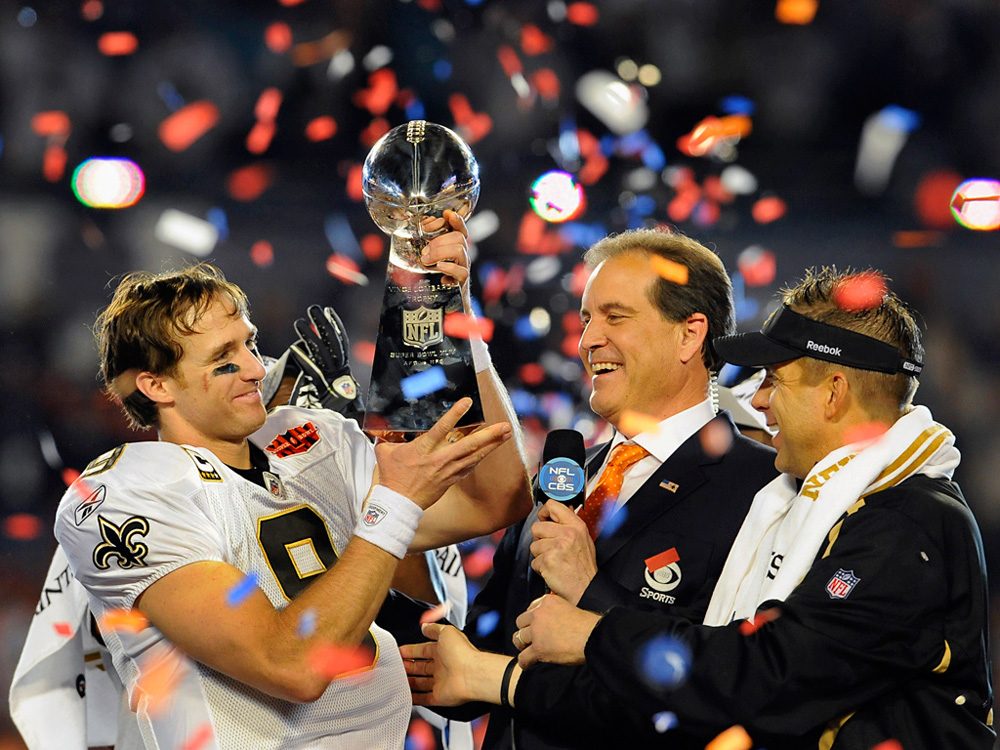
\includegraphics[max width=0.95\textwidth,
        max height=0.54000\textheight]{{Images/saints}.jpg}
    \end{center}
    \end{column}
    \end{columns}
}
\end{frame}
\begin{frame}[t]{Round 4 --- It happened in 2010 --- \mbox{Answer 3}}
\vspace{-0.5em}
\begin{block}{Question}
On February 12\textsuperscript{th}, the winter Olympic Games opened in which city?
\end{block}

\visible<2->{
    \begin{columns}[T,totalwidth=\linewidth]
    \begin{column}{0.32\linewidth}
    \begin{block}{Answer}
    Vancouver
    \end{block}
    \end{column}
    \begin{column}{0.65\linewidth}
    \begin{center}
    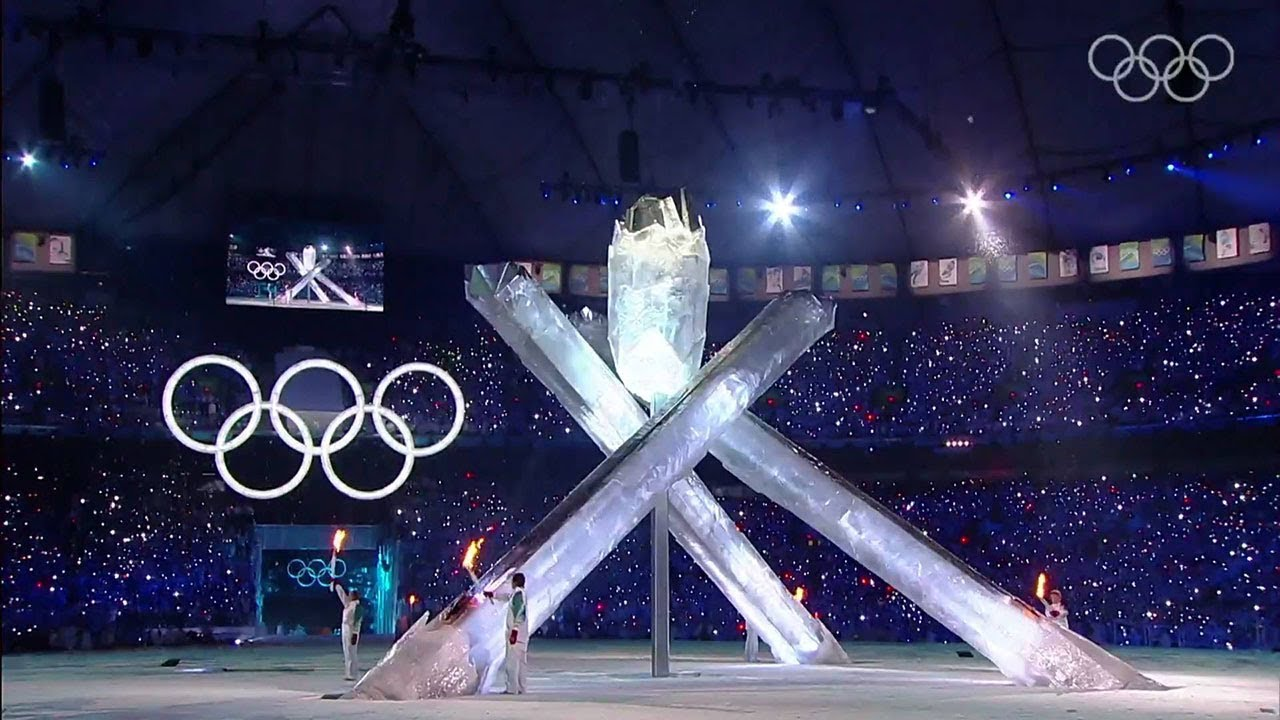
\includegraphics[max width=0.95\textwidth,
        max height=0.54000\textheight]{{Images/vancouver}.jpg}
    \end{center}
    \end{column}
    \end{columns}
}
\end{frame}
\begin{frame}[t]{Round 4 --- It happened in 2010 --- \mbox{Answer 4}}
\vspace{-0.5em}
\begin{block}{Question}
On April 14\textsuperscript{th}, the volcano Eyjafjallajökull began erupting. The eruption ultimately caused problems with air travel. In which country was the volcano located?
\end{block}

\visible<2->{
    \begin{columns}[T,totalwidth=\linewidth]
    \begin{column}{0.32\linewidth}
    \begin{block}{Answer}
    Iceland
    \end{block}
    \end{column}
    \begin{column}{0.65\linewidth}
    \begin{center}
    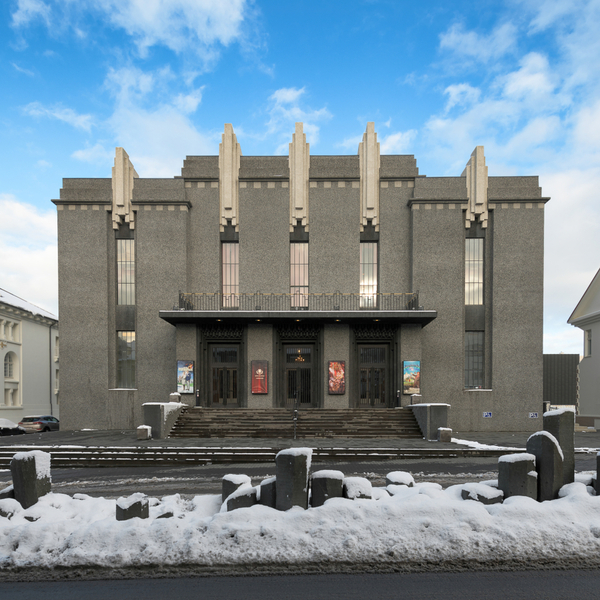
\includegraphics[max width=0.95\textwidth,
        max height=0.46000\textheight]{{Images/iceland}.jpg}
    \end{center}
    \end{column}
    \end{columns}
}
\end{frame}
\begin{frame}[t]{Round 4 --- It happened in 2010 --- \mbox{Answer 5}}
\vspace{-0.5em}
\begin{block}{Question}
What was the name of the drilling rig that exploded in the Gulf of Mexico on April 20\textsuperscript{th}?
\end{block}

\visible<2->{
    \begin{columns}[T,totalwidth=\linewidth]
    \begin{column}{0.32\linewidth}
    \begin{block}{Answer}
    The Deepwater Horizon
    \end{block}
    \end{column}
    \begin{column}{0.65\linewidth}
    \begin{center}
    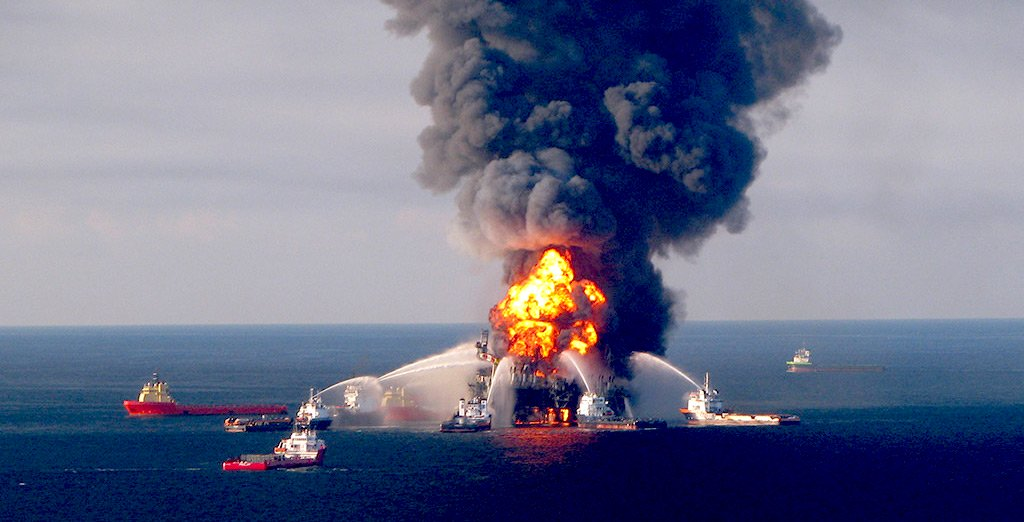
\includegraphics[max width=0.95\textwidth,
        max height=0.50000\textheight]{{Images/deepwater}.jpg}
    \end{center}
    \end{column}
    \end{columns}
}
\end{frame}
\begin{frame}[t]{Round 4 --- It happened in 2010 --- \mbox{Answer 6}}
\vspace{-0.5em}
\begin{block}{Question}
Who became British Prime Minister on May 11\textsuperscript{th}?
\end{block}

\visible<2->{
    \begin{columns}[T,totalwidth=\linewidth]
    \begin{column}{0.32\linewidth}
    \begin{block}{Answer}
    David Cameron
    \end{block}
    \end{column}
    \begin{column}{0.65\linewidth}
    \begin{center}
    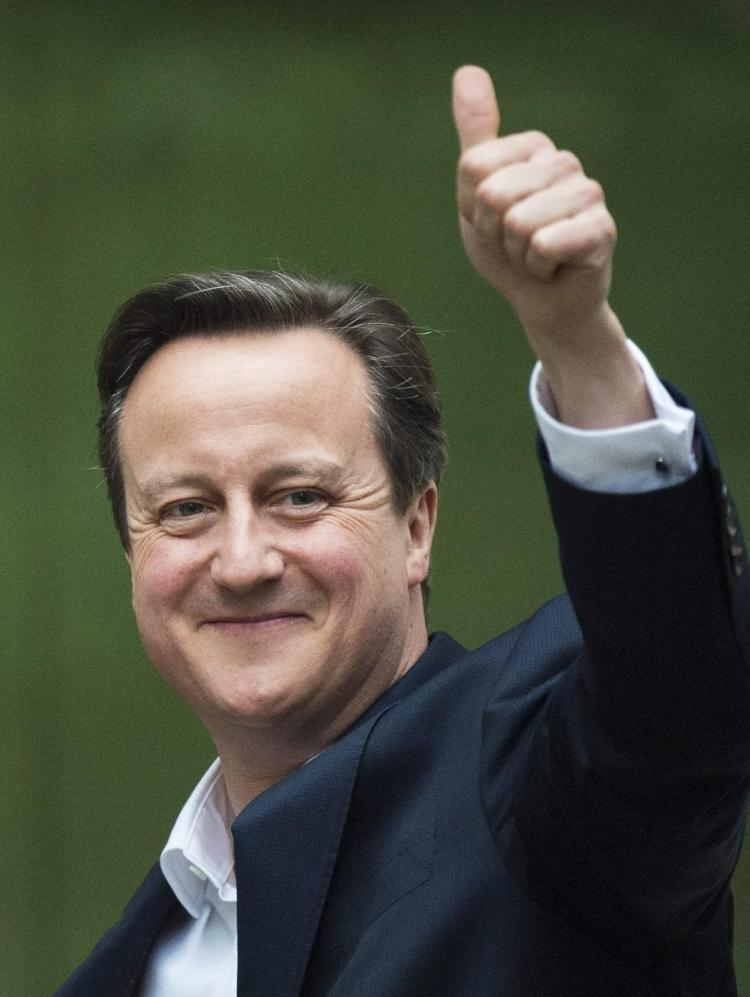
\includegraphics[max width=0.95\textwidth,
        max height=0.54000\textheight]{{Images/cameron}.jpg}
    \end{center}
    \end{column}
    \end{columns}
}
\end{frame}
\begin{frame}[t]{Round 4 --- It happened in 2010 --- \mbox{Answer 7}}
\vspace{-0.5em}
\begin{block}{Question}
On May 29\textsuperscript{th}, which MLB pitcher became the 20\textsuperscript{th} MLB pitcher to throw a perfect game?
\end{block}

\visible<2->{
    \begin{columns}[T,totalwidth=\linewidth]
    \begin{column}{0.32\linewidth}
    \begin{block}{Answer}
    Roy Halladay (Philadelphia Phillies)
    \end{block}
    \end{column}
    \begin{column}{0.65\linewidth}
    \begin{center}
    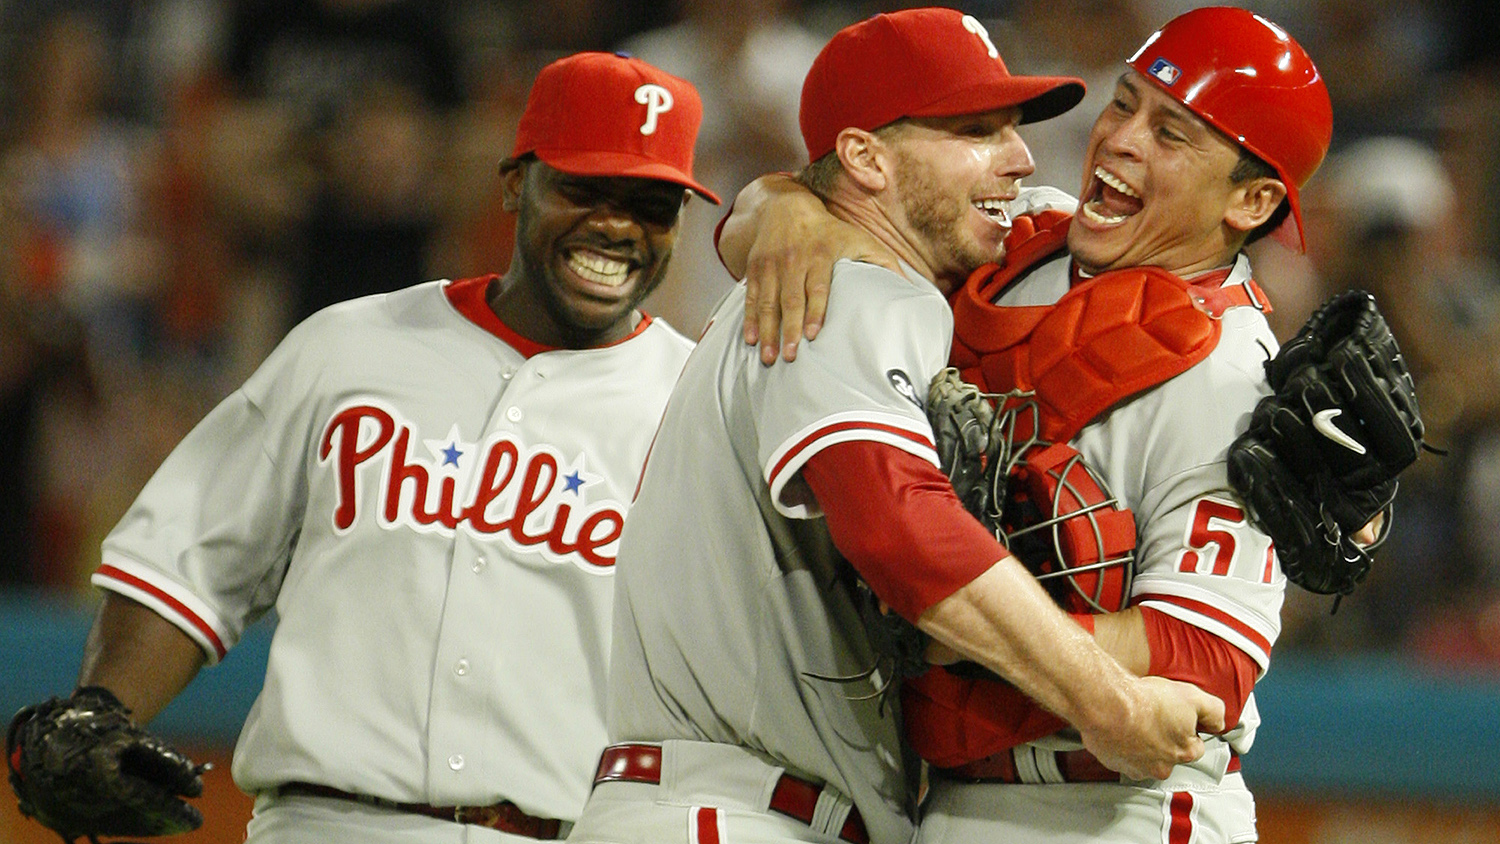
\includegraphics[max width=0.95\textwidth,
        max height=0.50000\textheight]{{Images/halladay}.jpg}
    \end{center}
    \end{column}
    \end{columns}
}
\end{frame}
\begin{frame}[t]{Round 4 --- It happened in 2010 --- \mbox{Answer 8}}
\vspace{-0.5em}
\begin{block}{Question}
On July 3\textsuperscript{rd}, who won the Wimbledon Women's Championship?
\end{block}

\visible<2->{
    \begin{columns}[T,totalwidth=\linewidth]
    \begin{column}{0.32\linewidth}
    \begin{block}{Answer}
    Serena Williams
    \end{block}
    \end{column}
    \begin{column}{0.65\linewidth}
    \begin{center}
    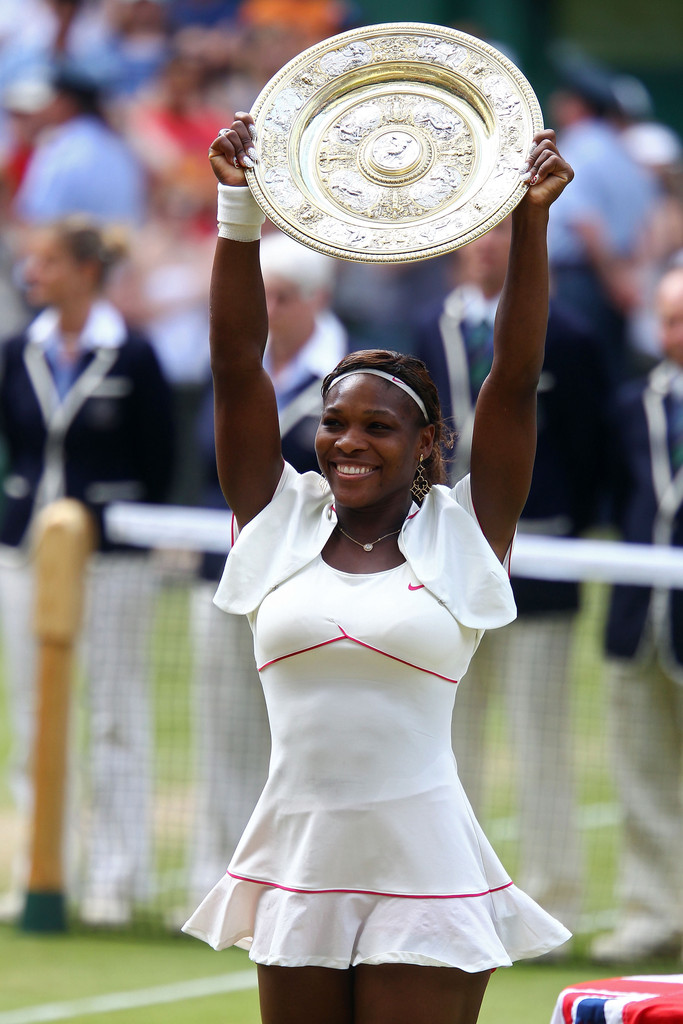
\includegraphics[max width=0.95\textwidth,
        max height=0.54000\textheight]{{Images/serena}.jpg}
    \end{center}
    \end{column}
    \end{columns}
}
\end{frame}
\begin{frame}[t]{Round 4 --- It happened in 2010 --- \mbox{Answer 9}}
\vspace{-0.5em}
\begin{block}{Question}
On November 1\textsuperscript{st}, which team won the World Series?
\end{block}

\visible<2->{
    \begin{columns}[T,totalwidth=\linewidth]
    \begin{column}{0.32\linewidth}
    \begin{block}{Answer}
    San Francisco Giants
    \end{block}
    \end{column}
    \begin{column}{0.65\linewidth}
    \begin{center}
    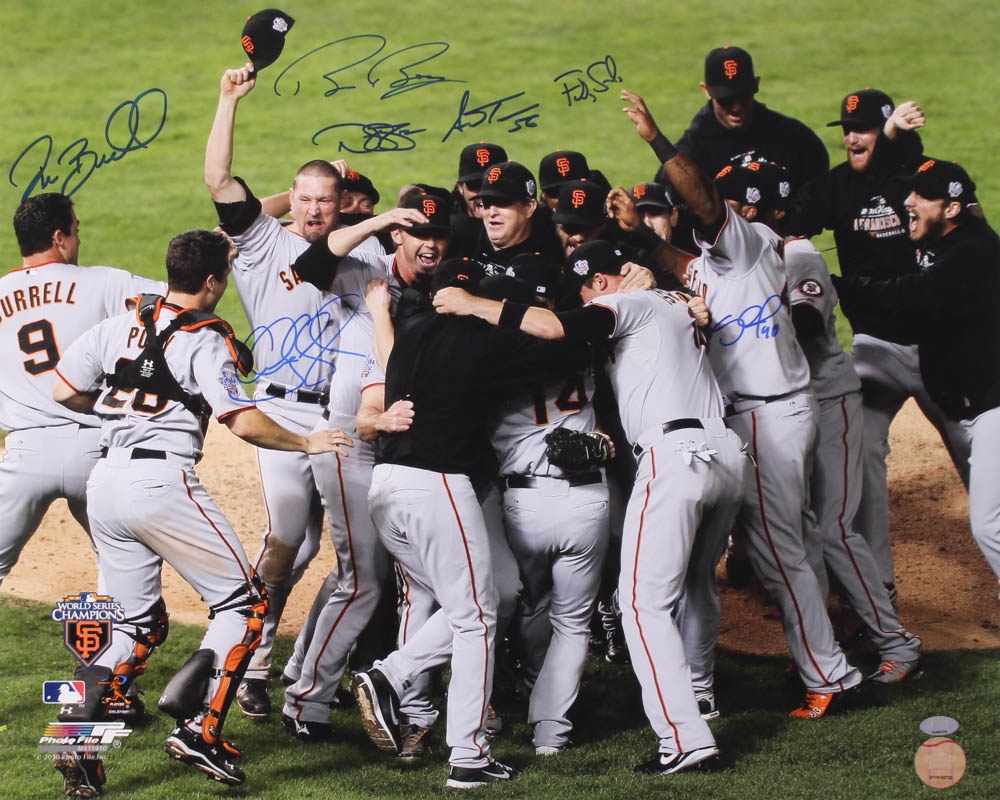
\includegraphics[max width=0.95\textwidth,
        max height=0.54000\textheight]{{Images/bumgarner}.jpg}
    \end{center}
    \end{column}
    \end{columns}
}
\end{frame}
\begin{frame}[t]{Round 4 --- It happened in 2010 --- \mbox{Answer 10}}
\vspace{-0.5em}
\begin{block}{Question}
On December 10\textsuperscript{th}, who was awarded the Nobel Peace Prize while imprisoned?
\end{block}

\visible<2->{
    \begin{columns}[T,totalwidth=\linewidth]
    \begin{column}{0.32\linewidth}
    \begin{block}{Answer}
    Chinese human rights activist Liu Xiaobo
    \end{block}
    \end{column}
    \begin{column}{0.65\linewidth}
    \begin{center}
    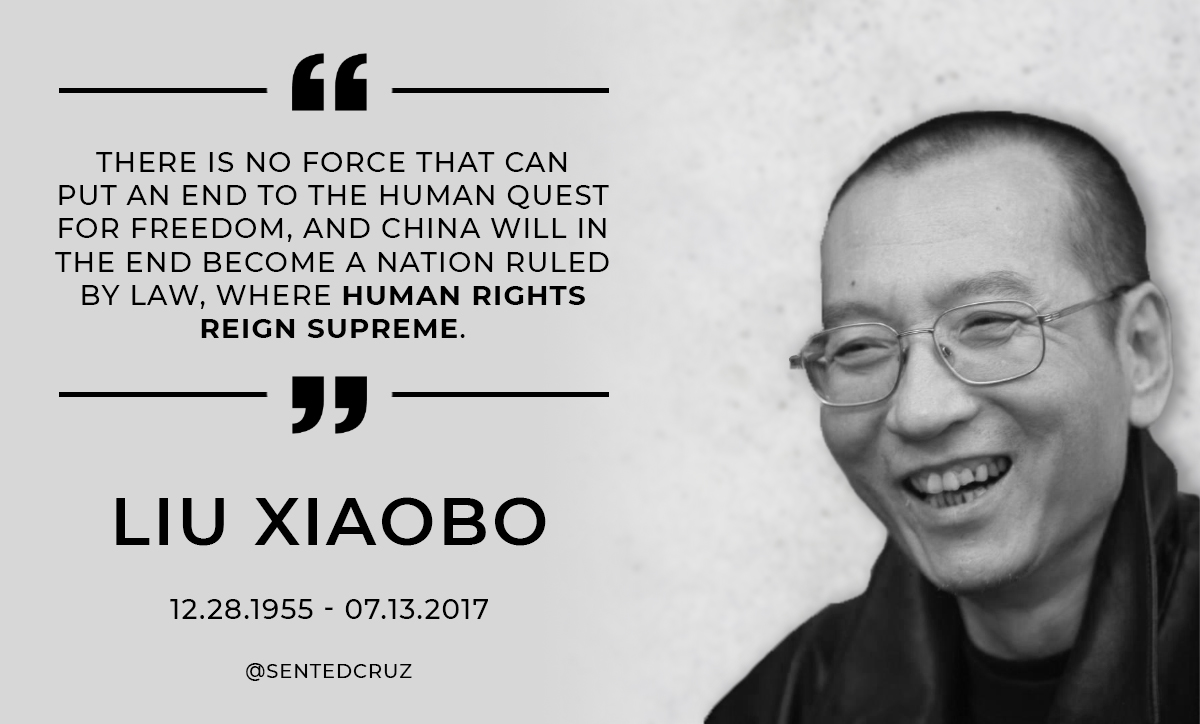
\includegraphics[max width=0.95\textwidth,
        max height=0.54000\textheight]{{Images/xiaobo}.jpg}
    \end{center}
    \end{column}
    \end{columns}
}
\end{frame}
\def\thisSectionName{Under the Sea}
\section{Round 5}
\subsection*{Q1}
\begin{frame}[t]{Round 5 --- Under the Sea --- \mbox{Question 1}}
\vspace{-0.5em}
\begin{block}{Question}
What is the name of the deepest trench in the ocean?
\end{block}
\end{frame}
\subsection*{Q2}
\begin{frame}[t]{Round 5 --- Under the Sea --- \mbox{Question 2}}
\vspace{-0.5em}
\begin{columns}[T,totalwidth=\linewidth]
\begin{column}{0.32\linewidth}
\begin{block}{Question}
What is the name of the filter, visible here as the hairy curtain in the whale's mouth, that some species of whale use to filter small animals out of seawater?
\end{block}
\end{column}
\begin{column}{0.65\linewidth}
\begin{center}
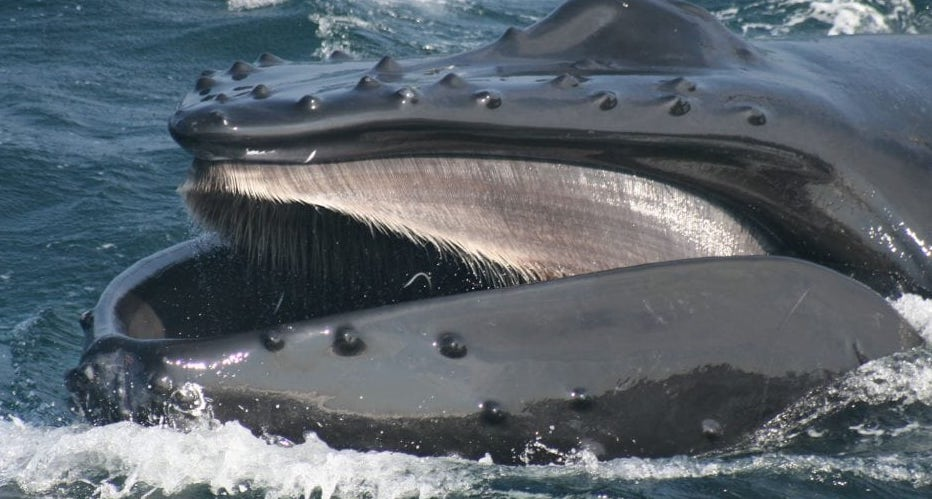
\includegraphics[max width=0.95\textwidth,max height=0.7\textheight]{{Images/baleen}.jpg}
\end{center}
\end{column}
\end{columns}
\end{frame}
\subsection*{Q3}
\begin{frame}[t]{Round 5 --- Under the Sea --- \mbox{Question 3}}
\vspace{-0.5em}
\begin{block}{Question}
Unlike most other vertebrates, sharks' bones are not rigid, as they don't contain calcium; instead, their bones are made of which flexible substance?
\end{block}
\end{frame}
\subsection*{Q4}
\begin{frame}[t]{Round 5 --- Under the Sea --- \mbox{Question 4}}
\vspace{-0.5em}
\begin{block}{Question}
Which of the Seven Wonders of the Ancient World is the only one that, today, has a significant proportion of its remains underwater?
\end{block}
\end{frame}
\subsection*{Q5}
\begin{frame}[t]{Round 5 --- Under the Sea --- \mbox{Question 5}}
\vspace{-0.5em}
\begin{block}{Question}
To help create artificial reefs, New York City has dumped over 2,500 of what large object into the ocean?
\end{block}
\end{frame}
\subsection*{Q6}
\begin{frame}[t]{Round 5 --- Under the Sea --- \mbox{Question 6}}
\vspace{-0.5em}
\begin{block}{Question}
``Benthos'' refers to the community of organisms that inhabit which part of the ocean?
\end{block}
\end{frame}
\subsection*{Q7}
\begin{frame}[t]{Round 5 --- Under the Sea --- \mbox{Question 7}}
\vspace{-0.5em}
\begin{block}{Question}
In which ocean is the longest underwater mountain chain located?
\end{block}
\end{frame}
\subsection*{Q8}
\begin{frame}[t]{Round 5 --- Under the Sea --- \mbox{Question 8}}
\vspace{-0.5em}
\begin{columns}[T,totalwidth=\linewidth]
\begin{column}{0.32\linewidth}
\begin{block}{Question}
These pictures are all of the same species of octopus, which has evolved to imitate other underwater creatures. What is the (apt!) name of this species of octopus?
\end{block}
\end{column}
\begin{column}{0.65\linewidth}
\begin{center}
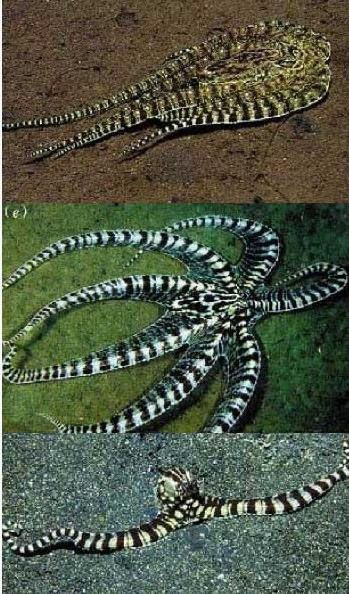
\includegraphics[max width=0.95\textwidth,max height=0.7\textheight]{{Images/mimic}.jpg}
\end{center}
\end{column}
\end{columns}
\end{frame}
\subsection*{Q9}
\begin{frame}[t]{Round 5 --- Under the Sea --- \mbox{Question 9}}
\vspace{-0.5em}
\begin{block}{Question}
Despite the lack of sunlight there, the deepest parts of the ocean are still home to living creatures thanks to which geological features in the ocean floor that eject hot, nutrient-rich water?
\end{block}
\end{frame}
\subsection*{Q10}
\begin{frame}[t]{Round 5 --- Under the Sea --- \mbox{Question 10}}
\vspace{-0.5em}
\begin{block}{Question}
The name of the brownish color sepia comes from the Ancient Greek word for the underwater animal whose ink was used to make the first sepia-colored ink. What kind of animal's ink did they use?
\end{block}
\end{frame}
\subsection{Answers}
\begin{frame}[t]{Round 5 --- Under the Sea --- \mbox{Answer 1}}
\vspace{-0.5em}
\begin{block}{Question}
What is the name of the deepest trench in the ocean?
\end{block}

\visible<2->{
    \begin{columns}[T,totalwidth=\linewidth]
    \begin{column}{0.32\linewidth}
    \begin{block}{Answer}
    Mariana Trench or Marianas Trench
    \end{block}
    \end{column}
    \begin{column}{0.65\linewidth}
    \begin{center}
    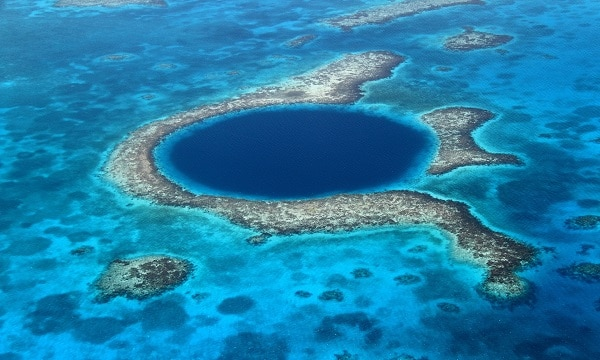
\includegraphics[max width=0.95\textwidth,
        max height=0.54000\textheight]{{Images/mariana}.jpeg}
    \end{center}
    \end{column}
    \end{columns}
}
\end{frame}
\begin{frame}[t]{Round 5 --- Under the Sea --- \mbox{Answer 2}}
\vspace{-0.5em}
\begin{columns}[T,totalwidth=\linewidth]
\begin{column}{0.32\linewidth}
\begin{block}{Question}
What is the name of the filter, visible here as the hairy curtain in the whale's mouth, that some species of whale use to filter small animals out of seawater?
\end{block}
\visible<2->{
    \begin{block}{Answer}
    Baleen / Whalebone
    \end{block}
}
\end{column}
\begin{column}{0.65\linewidth}
\begin{center}
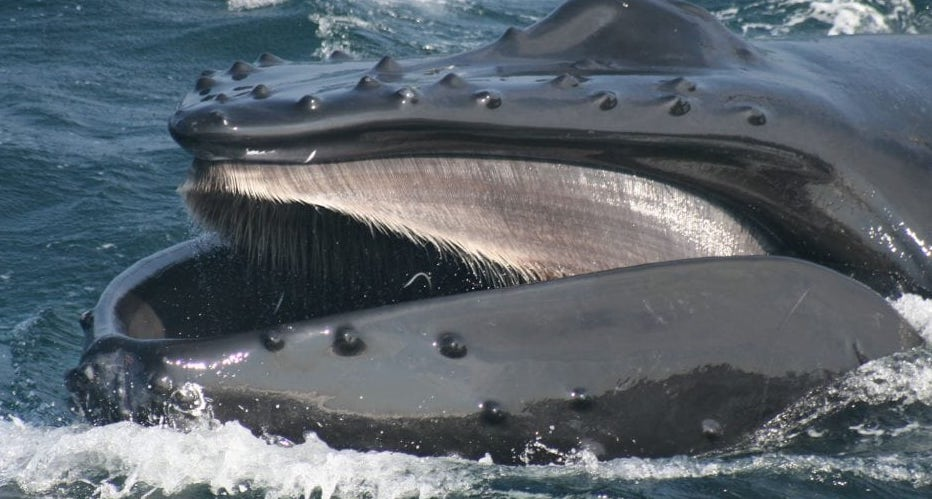
\includegraphics[max width=0.95\textwidth,max height=0.7\textheight]{{Images/baleen}.jpg}
\end{center}
\end{column}
\end{columns}
\end{frame}
\begin{frame}[t]{Round 5 --- Under the Sea --- \mbox{Answer 3}}
\vspace{-0.5em}
\begin{block}{Question}
Unlike most other vertebrates, sharks' bones are not rigid, as they don't contain calcium; instead, their bones are made of which flexible substance?
\end{block}

\visible<2->{
    \begin{columns}[T,totalwidth=\linewidth]
    \begin{column}{0.32\linewidth}
    \begin{block}{Answer}
    Cartilage
    \end{block}
    \end{column}
    \begin{column}{0.65\linewidth}
    \begin{center}
    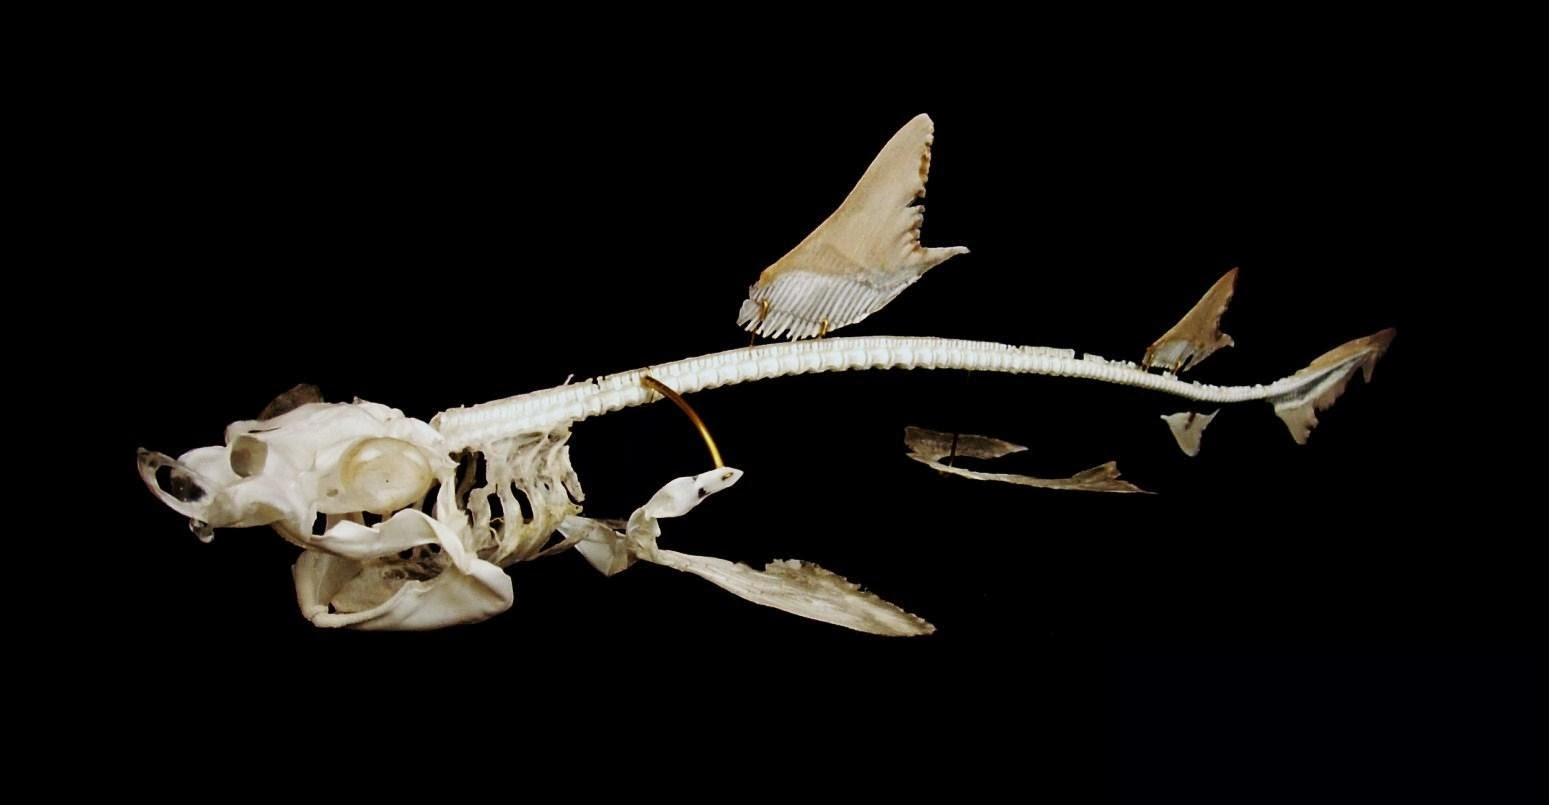
\includegraphics[max width=0.95\textwidth,
        max height=0.50000\textheight]{{Images/cartilage}.jpg}
    \end{center}
    \end{column}
    \end{columns}
}
\end{frame}
\begin{frame}[t]{Round 5 --- Under the Sea --- \mbox{Answer 4}}
\vspace{-0.5em}
\begin{block}{Question}
Which of the Seven Wonders of the Ancient World is the only one that, today, has a significant proportion of its remains underwater?
\end{block}

\visible<2->{
    \begin{columns}[T,totalwidth=\linewidth]
    \begin{column}{0.32\linewidth}
    \begin{block}{Answer}
    The Lighthouse of Alexandria
    \end{block}
    \end{column}
    \begin{column}{0.65\linewidth}
    \begin{center}
    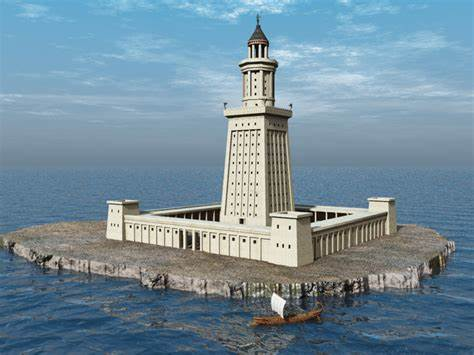
\includegraphics[max width=0.95\textwidth,
        max height=0.50000\textheight]{{Images/alexandria}.jpeg}
    \end{center}
    \end{column}
    \end{columns}
}
\end{frame}
\begin{frame}[t]{Round 5 --- Under the Sea --- \mbox{Answer 5}}
\vspace{-0.5em}
\begin{block}{Question}
To help create artificial reefs, New York City has dumped over 2,500 of what large object into the ocean?
\end{block}

\visible<2->{
    \begin{columns}[T,totalwidth=\linewidth]
    \begin{column}{0.32\linewidth}
    \begin{block}{Answer}
    Subway cars
    \end{block}
    \end{column}
    \begin{column}{0.65\linewidth}
    \begin{center}
    \includegraphics[max width=0.95\textwidth,
        max height=0.50000\textheight]{{Images/subwayreef}.jpg}
    \end{center}
    \end{column}
    \end{columns}
}
\end{frame}
\begin{frame}[t]{Round 5 --- Under the Sea --- \mbox{Answer 6}}
\vspace{-0.5em}
\begin{block}{Question}
``Benthos'' refers to the community of organisms that inhabit which part of the ocean?
\end{block}

\visible<2->{
    \begin{columns}[T,totalwidth=\linewidth]
    \begin{column}{0.32\linewidth}
    \begin{block}{Answer}
    The benthic zone / the ocean floor / the bottom 
    \end{block}
    \end{column}
    \begin{column}{0.65\linewidth}
    \begin{center}
    \includegraphics[max width=0.95\textwidth,
        max height=0.54000\textheight]{{Images/benthic}.jpg}
    \end{center}
    \end{column}
    \end{columns}
}
\end{frame}
\begin{frame}[t]{Round 5 --- Under the Sea --- \mbox{Answer 7}}
\vspace{-0.5em}
\begin{block}{Question}
In which ocean is the longest underwater mountain chain located?
\end{block}

\visible<2->{
    \begin{columns}[T,totalwidth=\linewidth]
    \begin{column}{0.32\linewidth}
    \begin{block}{Answer}
    The Atlantic (the Mid-Atlantic Ridge)
    \end{block}
    \end{column}
    \begin{column}{0.65\linewidth}
    \begin{center}
    \includegraphics[max width=0.95\textwidth,
        max height=0.54000\textheight]{{Images/atlanticridge}.jpg}
    \end{center}
    \end{column}
    \end{columns}
}
\end{frame}
\begin{frame}[t]{Round 5 --- Under the Sea --- \mbox{Answer 8}}
\vspace{-0.5em}
\begin{columns}[T,totalwidth=\linewidth]
\begin{column}{0.32\linewidth}
\begin{block}{Question}
These pictures are all of the same species of octopus, which has evolved to imitate other underwater creatures. What is the (apt!) name of this species of octopus?
\end{block}
\visible<2->{
    \begin{block}{Answer}
    Mimic octopus
    \end{block}
}
\end{column}
\begin{column}{0.65\linewidth}
\begin{center}
\includegraphics[max width=0.95\textwidth,max height=0.7\textheight]{{Images/mimic}.jpg}
\end{center}
\end{column}
\end{columns}
\end{frame}
\begin{frame}[t]{Round 5 --- Under the Sea --- \mbox{Answer 9}}
\vspace{-0.5em}
\begin{block}{Question}
Despite the lack of sunlight there, the deepest parts of the ocean are still home to living creatures thanks to which geological features in the ocean floor that eject hot, nutrient-rich water?
\end{block}

\visible<2->{
    \begin{columns}[T,totalwidth=\linewidth]
    \begin{column}{0.32\linewidth}
    \begin{block}{Answer}
    Hydrothermal vents
    \end{block}
    \end{column}
    \begin{column}{0.65\linewidth}
    \begin{center}
    \includegraphics[max width=0.95\textwidth,
        max height=0.46000\textheight]{{Images/hydrothermal}.jpg}
    \end{center}
    \end{column}
    \end{columns}
}
\end{frame}
\begin{frame}[t]{Round 5 --- Under the Sea --- \mbox{Answer 10}}
\vspace{-0.5em}
\begin{block}{Question}
The name of the brownish color sepia comes from the Ancient Greek word for the underwater animal whose ink was used to make the first sepia-colored ink. What kind of animal's ink did they use?
\end{block}

\visible<2->{
    \begin{columns}[T,totalwidth=\linewidth]
    \begin{column}{0.32\linewidth}
    \begin{block}{Answer}
    Cuttlefish
    \end{block}
    \end{column}
    \begin{column}{0.65\linewidth}
    \begin{center}
    \includegraphics[max width=0.95\textwidth,
        max height=0.46000\textheight]{{Images/cuttlefish}.jpg}
    \end{center}
    \end{column}
    \end{columns}
}
\end{frame}
\def\thisSectionName{Myths and Legends}
\section{Round 6}
\subsection*{Q1}
\begin{frame}[t]{Round 6 --- Myths and Legends --- \mbox{Question 1}}
\vspace{-0.5em}
\begin{columns}[T,totalwidth=\linewidth]
\begin{column}{0.32\linewidth}
\begin{block}{Question}
Which Christian saint is depicted here slaying a dragon?
\end{block}
\end{column}
\begin{column}{0.65\linewidth}
\begin{center}
\includegraphics[max width=0.95\textwidth,max height=0.7\textheight]{{Images/georgedragon}.jpg}
\end{center}
\end{column}
\end{columns}
\end{frame}
\subsection*{Q2}
\begin{frame}[t]{Round 6 --- Myths and Legends --- \mbox{Question 2}}
\vspace{-0.5em}
\begin{block}{Question}
In Norse mythology, Odin had a pair of what kind of birds that would report the goings-on of the world to him?
\end{block}
\end{frame}
\subsection*{Q3}
\begin{frame}[t]{Round 6 --- Myths and Legends --- \mbox{Question 3}}
\vspace{-0.5em}
\begin{block}{Question}
In the \emph{Odyssey}, when the cyclops Polyphemus asks Odysseus his name, what does Odysseus say his name is?
\end{block}
\end{frame}
\subsection*{Q4}
\begin{frame}[t]{Round 6 --- Myths and Legends --- \mbox{Question 4}}
\vspace{-0.5em}
\begin{columns}[T,totalwidth=\linewidth]
\begin{column}{0.32\linewidth}
\begin{block}{Question}
The ancient Egyptian symbol here, called a \emph{wadjet}, is also known as the eye of which Egyptian god?
\end{block}
\end{column}
\begin{column}{0.65\linewidth}
\begin{center}
\includegraphics[max width=0.95\textwidth,max height=0.7\textheight]{{Images/wadget}.png}
\end{center}
\end{column}
\end{columns}
\end{frame}
\subsection*{Q5}
\begin{frame}[t]{Round 6 --- Myths and Legends --- \mbox{Question 5}}
\vspace{-0.5em}
\begin{block}{Question}
Which of King Arthur's knights battled the Green Knight?
\end{block}
\end{frame}
\subsection*{Q6}
\begin{frame}[t]{Round 6 --- Myths and Legends --- \mbox{Question 6}}
\vspace{-0.5em}
\begin{block}{Question}
According to Greek mythology, who was the very first human woman, who, having been adorned with gifts by the gods, was named the Greek for ``all-gifted''?
\end{block}
\end{frame}
\subsection*{Q7}
\begin{frame}[t]{Round 6 --- Myths and Legends --- \mbox{Question 7}}
\vspace{-0.5em}
\begin{block}{Question}
What is the name of Paul Bunyan's ox companion?
\end{block}
\end{frame}
\subsection*{Q8}
\begin{frame}[t]{Round 6 --- Myths and Legends --- \mbox{Question 8}}
\vspace{-0.5em}
\begin{columns}[T,totalwidth=\linewidth]
\begin{column}{0.32\linewidth}
\begin{block}{Question}
Referring to \emph{Hansel and Gretel}, what is the name for the software feature that shows the path you've taken to arrive at the current page?
\end{block}
\end{column}
\begin{column}{0.65\linewidth}
\begin{center}
\includegraphics[max width=0.95\textwidth,max height=0.7\textheight]{{Images/breadcrumbs}.png}
\end{center}
\end{column}
\end{columns}
\end{frame}
\subsection*{Q9}
\begin{frame}[t]{Round 6 --- Myths and Legends --- \mbox{Question 9}}
\vspace{-0.5em}
\begin{block}{Question}
In Jewish mythology, what is the term for a humanoid being formed from clay who acts mindlessly at its creator's bidding?
\end{block}
\end{frame}
\subsection*{Q10}
\begin{frame}[t]{Round 6 --- Myths and Legends --- \mbox{Question 10}}
\vspace{-0.5em}
\begin{block}{Question}
In Chinese mythology, which auspicious beings are believed to control water and are responsible for water-related weather phenomena?
\end{block}
\end{frame}
\subsection{Answers}
\begin{frame}[t]{Round 6 --- Myths and Legends --- \mbox{Answer 1}}
\vspace{-0.5em}
\begin{columns}[T,totalwidth=\linewidth]
\begin{column}{0.32\linewidth}
\begin{block}{Question}
Which Christian saint is depicted here slaying a dragon?
\end{block}
\visible<2->{
    \begin{block}{Answer}
    Saint George
    \end{block}
}
\end{column}
\begin{column}{0.65\linewidth}
\begin{center}
\includegraphics[max width=0.95\textwidth,max height=0.7\textheight]{{Images/georgedragon}.jpg}
\end{center}
\end{column}
\end{columns}
\end{frame}
\begin{frame}[t]{Round 6 --- Myths and Legends --- \mbox{Answer 2}}
\vspace{-0.5em}
\begin{block}{Question}
In Norse mythology, Odin had a pair of what kind of birds that would report the goings-on of the world to him?
\end{block}

\visible<2->{
    \begin{columns}[T,totalwidth=\linewidth]
    \begin{column}{0.32\linewidth}
    \begin{block}{Answer}
    Ravens
    \end{block}
    \end{column}
    \begin{column}{0.65\linewidth}
    \begin{center}
    \includegraphics[max width=0.95\textwidth,
        max height=0.50000\textheight]{{Images/odinravens}.jpg}
    \end{center}
    \end{column}
    \end{columns}
}
\end{frame}
\begin{frame}[t]{Round 6 --- Myths and Legends --- \mbox{Answer 3}}
\vspace{-0.5em}
\begin{block}{Question}
In the \emph{Odyssey}, when the cyclops Polyphemus asks Odysseus his name, what does Odysseus say his name is?
\end{block}

\visible<2->{
    \begin{columns}[T,totalwidth=\linewidth]
    \begin{column}{0.32\linewidth}
    \begin{block}{Answer}
    Nobody
    \end{block}
    \end{column}
    \begin{column}{0.65\linewidth}
    \begin{center}
    \includegraphics[max width=0.95\textwidth,
        max height=0.50000\textheight]{{Images/nobody}.jpg}
    \end{center}
    \end{column}
    \end{columns}
}
\end{frame}
\begin{frame}[t]{Round 6 --- Myths and Legends --- \mbox{Answer 4}}
\vspace{-0.5em}
\begin{columns}[T,totalwidth=\linewidth]
\begin{column}{0.38\linewidth}
\begin{block}{Question}
The ancient Egyptian symbol here, called a \emph{wadjet}, is also known as the eye of which Egyptian god?
\end{block}
\end{column}
\begin{column}{0.6\linewidth}
\begin{center}
\includegraphics[max width=0.95\textwidth,max height=0.35\textheight]{{Images/wadget}.png}
\end{center}
\end{column}
\end{columns}

\visible<2->{
    \begin{columns}[T,totalwidth=\linewidth]
    \begin{column}{0.38\linewidth}
    \begin{block}{Answer}
    Horus
    \end{block}
    \end{column}
    \begin{column}{0.6\linewidth}
    \begin{center}
    \includegraphics[max width=0.95\textwidth,
        max height=0.34\textheight]{{Images/horus}.png}
    \end{center}
    \end{column}
    \end{columns}
}
\end{frame}
\begin{frame}[t]{Round 6 --- Myths and Legends --- \mbox{Answer 5}}
\vspace{-0.5em}
\begin{block}{Question}
Which of King Arthur's knights battled the Green Knight?
\end{block}

\visible<2->{
    \begin{columns}[T,totalwidth=\linewidth]
    \begin{column}{0.32\linewidth}
    \begin{block}{Answer}
    (Sir) Gawain
    \end{block}
    \end{column}
    \begin{column}{0.65\linewidth}
    \begin{center}
    \includegraphics[max width=0.95\textwidth,
        max height=0.54000\textheight]{{Images/gawain}.jpg}
    \end{center}
    \end{column}
    \end{columns}
}
\end{frame}
\begin{frame}[t]{Round 6 --- Myths and Legends --- \mbox{Answer 6}}
\vspace{-0.5em}
\begin{block}{Question}
According to Greek mythology, who was the very first human woman, who, having been adorned with gifts by the gods, was named the Greek for ``all-gifted''?
\end{block}

\visible<2->{
    \begin{columns}[T,totalwidth=\linewidth]
    \begin{column}{0.32\linewidth}
    \begin{block}{Answer}
    Pandora
    \end{block}
    \end{column}
    \begin{column}{0.65\linewidth}
    \begin{center}
    \includegraphics[max width=0.95\textwidth,
        max height=0.46000\textheight]{{Images/pandora}.jpg}
    \end{center}
    \end{column}
    \end{columns}
}
\end{frame}
\begin{frame}[t]{Round 6 --- Myths and Legends --- \mbox{Answer 7}}
\vspace{-0.5em}
\begin{block}{Question}
What is the name of Paul Bunyan's ox companion?
\end{block}

\visible<2->{
    \begin{columns}[T,totalwidth=\linewidth]
    \begin{column}{0.32\linewidth}
    \begin{block}{Answer}
    Babe (the blue ox)
    \end{block}
    \end{column}
    \begin{column}{0.65\linewidth}
    \begin{center}
    \includegraphics[max width=0.95\textwidth,
        max height=0.58000\textheight]{{Images/bunyan}.jpg}
    \end{center}
    \end{column}
    \end{columns}
}
\end{frame}
\begin{frame}[t]{Round 6 --- Myths and Legends --- \mbox{Answer 8}}
\vspace{-0.5em}
\begin{columns}[T,totalwidth=\linewidth]
\begin{column}{0.38\linewidth}
\begin{block}{Question}
Referring to \emph{Hansel and Gretel}, what is the name for the software feature that shows the path you've taken to arrive at the current page?
\end{block}
\end{column}
\begin{column}{0.6\linewidth}
\begin{center}
\includegraphics[max width=0.95\textwidth,max height=0.35\textheight]{{Images/breadcrumbs}.png}
\end{center}
\end{column}
\end{columns}

\visible<2->{
    \begin{columns}[T,totalwidth=\linewidth]
    \begin{column}{0.38\linewidth}
    \begin{block}{Answer}
    Breadcrumbs
    \end{block}
    \end{column}
    \begin{column}{0.6\linewidth}
    \begin{center}
    \includegraphics[max width=0.95\textwidth,
        max height=0.34\textheight]{{Images/hanselgretel}.jpg}
    \end{center}
    \end{column}
    \end{columns}
}
\end{frame}
\begin{frame}[t]{Round 6 --- Myths and Legends --- \mbox{Answer 9}}
\vspace{-0.5em}
\begin{block}{Question}
In Jewish mythology, what is the term for a humanoid being formed from clay who acts mindlessly at its creator's bidding?
\end{block}

\visible<2->{
    \begin{columns}[T,totalwidth=\linewidth]
    \begin{column}{0.32\linewidth}
    \begin{block}{Answer}
    Golem
    \end{block}
    \end{column}
    \begin{column}{0.65\linewidth}
    \begin{center}
    \includegraphics[max width=0.95\textwidth,
        max height=0.50000\textheight]{{Images/golem}.jpg}
    \end{center}
    \end{column}
    \end{columns}
}
\end{frame}
\begin{frame}[t]{Round 6 --- Myths and Legends --- \mbox{Answer 10}}
\vspace{-0.5em}
\begin{block}{Question}
In Chinese mythology, which auspicious beings are believed to control water and are responsible for water-related weather phenomena?
\end{block}

\visible<2->{
    \begin{columns}[T,totalwidth=\linewidth]
    \begin{column}{0.32\linewidth}
    \begin{block}{Answer}
    Dragons
    \end{block}
    \end{column}
    \begin{column}{0.65\linewidth}
    \begin{center}
    \includegraphics[max width=0.95\textwidth,
        max height=0.50000\textheight]{{Images/dragon}.jpg}
    \end{center}
    \end{column}
    \end{columns}
}
\end{frame}
\def\thisSectionName{Mexico, Our Friendly Neighbor to the South}
\section{Round 7}
\subsection*{Q1}
\begin{frame}[t]{Round 7 --- Mexico, Our Friendly Neighbor to the South --- \mbox{Question 1}}
\vspace{-0.5em}
\begin{block}{Question}
What dog breed has the same name as a Mexican state?
\end{block}
\end{frame}
\subsection*{Q2}
\begin{frame}[t]{Round 7 --- Mexico, Our Friendly Neighbor to the South --- \mbox{Question 2}}
\vspace{-0.5em}
\begin{block}{Question}
Mexico City was built on the site of which former Aztec city?
\end{block}
\end{frame}
\subsection*{Q3}
\begin{frame}[t]{Round 7 --- Mexico, Our Friendly Neighbor to the South --- \mbox{Question 3}}
\vspace{-0.5em}
\begin{block}{Question}
What colors are the three stripes on the Mexican flag?
\end{block}
\end{frame}
\subsection*{Q4}
\begin{frame}[t]{Round 7 --- Mexico, Our Friendly Neighbor to the South --- \mbox{Question 4}}
\vspace{-0.5em}
\begin{block}{Question}
To within 300 feet, what is the elevation of Mexico City?
\end{block}
\end{frame}
\subsection*{Q5}
\begin{frame}[t]{Round 7 --- Mexico, Our Friendly Neighbor to the South --- \mbox{Question 5}}
\vspace{-0.5em}
\begin{block}{Question}
In 1910, under the guidance of Emiliano Zapata and Pancho Villa, Mexican peasants revolted against which dictator?
\end{block}
\end{frame}
\subsection*{Q6}
\begin{frame}[t]{Round 7 --- Mexico, Our Friendly Neighbor to the South --- \mbox{Question 6}}
\vspace{-0.5em}
\begin{block}{Question}
Who was the first actor to born in Mexico to win an Academy Award?
\end{block}
\end{frame}
\subsection*{Q7}
\begin{frame}[t]{Round 7 --- Mexico, Our Friendly Neighbor to the South --- \mbox{Question 7}}
\vspace{-0.5em}
\begin{columns}[T,totalwidth=\linewidth]
\begin{column}{0.32\linewidth}
\begin{block}{Question}
Which Mesoamerican people created the colossal stone head pictured here, which is about 10 feet tall?
\end{block}
\end{column}
\begin{column}{0.65\linewidth}
\begin{center}
\includegraphics[max width=0.95\textwidth,max height=0.7\textheight]{{Images/olmechead}.jpg}
\end{center}
\end{column}
\end{columns}
\end{frame}
\subsection*{Q8}
\begin{frame}[t]{Round 7 --- Mexico, Our Friendly Neighbor to the South --- \mbox{Question 8}}
\vspace{-0.5em}
\begin{block}{Question}
During which Aztec leader's reign did Spanish explorer Hernán Cortés arrive in the Americas?
\end{block}
\end{frame}
\subsection*{Q9}
\begin{frame}[t]{Round 7 --- Mexico, Our Friendly Neighbor to the South --- \mbox{Question 9}}
\vspace{-0.5em}
\begin{block}{Question}
According to the California Avocado Commission, on which Mexican holiday do Americans consume up to 81 million pounds of  avocados?
\end{block}
\end{frame}
\subsection*{Q10}
\begin{frame}[t]{Round 7 --- Mexico, Our Friendly Neighbor to the South --- \mbox{Question 10}}
\vspace{-0.5em}
\begin{block}{Question}
To within five million, what is the population of Mexico?
\end{block}
\end{frame}
\subsection{Answers}
\begin{frame}[t]{Round 7 --- Mexico, Our Friendly Neighbor to the South --- \mbox{Answer 1}}
\vspace{-0.5em}
\begin{block}{Question}
What dog breed has the same name as a Mexican state?
\end{block}

\visible<2->{
    \begin{columns}[T,totalwidth=\linewidth]
    \begin{column}{0.32\linewidth}
    \begin{block}{Answer}
    Chihuahua
    \end{block}
    \end{column}
    \begin{column}{0.65\linewidth}
    \begin{center}
    \includegraphics[max width=0.95\textwidth,
        max height=0.54000\textheight]{{Images/sombrero}.jpg}
    \end{center}
    \end{column}
    \end{columns}
}
\end{frame}
\begin{frame}[t]{Round 7 --- Mexico, Our Friendly Neighbor to the South --- \mbox{Answer 2}}
\vspace{-0.5em}
\begin{block}{Question}
Mexico City was built on the site of which former Aztec city?
\end{block}

\visible<2->{
    \begin{columns}[T,totalwidth=\linewidth]
    \begin{column}{0.32\linewidth}
    \begin{block}{Answer}
    Tenochtitlán
    \end{block}
    \end{column}
    \begin{column}{0.65\linewidth}
    \begin{center}
    \includegraphics[max width=0.95\textwidth,
        max height=0.54000\textheight]{{Images/tenochtitlan}.jpg}
    \end{center}
    \end{column}
    \end{columns}
}
\end{frame}
\begin{frame}[t]{Round 7 --- Mexico, Our Friendly Neighbor to the South --- \mbox{Answer 3}}
\vspace{-0.5em}
\begin{block}{Question}
What colors are the three stripes on the Mexican flag?
\end{block}

\visible<2->{
    \begin{columns}[T,totalwidth=\linewidth]
    \begin{column}{0.32\linewidth}
    \begin{block}{Answer}
    Green, white and red
    \end{block}
    \end{column}
    \begin{column}{0.65\linewidth}
    \begin{center}
    \includegraphics[max width=0.95\textwidth,
        max height=0.54000\textheight]{{Images/maxicanflag}.png}
    \end{center}
    \end{column}
    \end{columns}
}
\end{frame}
\begin{frame}[t]{Round 7 --- Mexico, Our Friendly Neighbor to the South --- \mbox{Answer 4}}
\vspace{-0.5em}
\begin{block}{Question}
To within 300 feet, what is the elevation of Mexico City?
\end{block}

\visible<2->{
    \begin{columns}[T,totalwidth=\linewidth]
    \begin{column}{0.32\linewidth}
    \begin{block}{Answer}
    7,382 feet above sea level (give yourself a point if you said anything between 7,082 and 7,682 feet)
    \end{block}
    \end{column}
    \begin{column}{0.65\linewidth}
    \begin{center}
    \includegraphics[max width=0.95\textwidth,
        max height=0.54000\textheight]{{Images/mexcity}.jpg}
    \end{center}
    \end{column}
    \end{columns}
}
\end{frame}
\begin{frame}[t]{Round 7 --- Mexico, Our Friendly Neighbor to the South --- \mbox{Answer 5}}
\vspace{-0.5em}
\begin{block}{Question}
In 1910, under the guidance of Emiliano Zapata and Pancho Villa, Mexican peasants revolted against which dictator?
\end{block}

\visible<2->{
    \begin{columns}[T,totalwidth=\linewidth]
    \begin{column}{0.32\linewidth}
    \begin{block}{Answer}
    Porfirio Díaz
    \end{block}
    \end{column}
    \begin{column}{0.65\linewidth}
    \begin{center}
    \includegraphics[max width=0.95\textwidth,
        max height=0.50000\textheight]{{Images/porfiriodiaz}.jpg}
    \end{center}
    \end{column}
    \end{columns}
}
\end{frame}
\begin{frame}[t]{Round 7 --- Mexico, Our Friendly Neighbor to the South --- \mbox{Answer 6}}
\vspace{-0.5em}
\begin{block}{Question}
Who was the first actor to born in Mexico to win an Academy Award?
\end{block}

\visible<2->{
    \begin{columns}[T,totalwidth=\linewidth]
    \begin{column}{0.32\linewidth}
    \begin{block}{Answer}
    Anthony Quinn, Best Supporting Actor, Viva Zapata! (1952)
    \end{block}
    \end{column}
    \begin{column}{0.65\linewidth}
    \begin{center}
    \includegraphics[max width=0.95\textwidth,
        max height=0.54000\textheight]{{Images/quinn}.jpg}
    \end{center}
    \end{column}
    \end{columns}
}
\end{frame}
\begin{frame}[t]{Round 7 --- Mexico, Our Friendly Neighbor to the South --- \mbox{Answer 7}}
\vspace{-0.5em}
\begin{columns}[T,totalwidth=\linewidth]
\begin{column}{0.32\linewidth}
\begin{block}{Question}
Which Mesoamerican people created the colossal stone head pictured here, which is about 10 feet tall?
\end{block}
\visible<2->{
    \begin{block}{Answer}
    The Olmec
    \end{block}
}
\end{column}
\begin{column}{0.65\linewidth}
\begin{center}
\includegraphics[max width=0.95\textwidth,max height=0.7\textheight]{{Images/olmechead}.jpg}
\end{center}
\end{column}
\end{columns}
\end{frame}
\begin{frame}[t]{Round 7 --- Mexico, Our Friendly Neighbor to the South --- \mbox{Answer 8}}
\vspace{-0.5em}
\begin{block}{Question}
During which Aztec leader's reign did Spanish explorer Hernán Cortés arrive in the Americas?
\end{block}

\visible<2->{
    \begin{columns}[T,totalwidth=\linewidth]
    \begin{column}{0.32\linewidth}
    \begin{block}{Answer}
    Montezuma or Moctezuma (technically II but we'll accept just the name without the suffix)
    \end{block}
    \end{column}
    \begin{column}{0.65\linewidth}
    \begin{center}
    \includegraphics[max width=0.95\textwidth,
        max height=0.54000\textheight]{{Images/montezuma}.jpg}
    \end{center}
    \end{column}
    \end{columns}
}
\end{frame}
\begin{frame}[t]{Round 7 --- Mexico, Our Friendly Neighbor to the South --- \mbox{Answer 9}}
\vspace{-0.5em}
\begin{block}{Question}
According to the California Avocado Commission, on which Mexican holiday do Americans consume up to 81 million pounds of  avocados?
\end{block}

\visible<2->{
    \begin{columns}[T,totalwidth=\linewidth]
    \begin{column}{0.32\linewidth}
    \begin{block}{Answer}
    Cinco de Mayo
    \end{block}
    \end{column}
    \begin{column}{0.65\linewidth}
    \begin{center}
    \includegraphics[max width=0.95\textwidth,
        max height=0.50000\textheight]{{Images/cincodeavo}.jpeg}
    \end{center}
    \end{column}
    \end{columns}
}
\end{frame}
\begin{frame}[t]{Round 7 --- Mexico, Our Friendly Neighbor to the South --- \mbox{Answer 10}}
\vspace{-0.5em}
\begin{block}{Question}
To within five million, what is the population of Mexico?
\end{block}

\visible<2->{
    \begin{columns}[T,totalwidth=\linewidth]
    \begin{column}{0.32\linewidth}
    \begin{block}{Answer}
    127 million (122 million-132 million will be accepted)
    \end{block}
    \end{column}
    \begin{column}{0.65\linewidth}
    \begin{center}
    \includegraphics[max width=0.95\textwidth,
        max height=0.54000\textheight]{{Images/mexicopop}.jpg}
    \end{center}
    \end{column}
    \end{columns}
}
\end{frame}
\def\thisSectionName{Famous Buildings}
\section{Round 8}
\subsection*{Q1}
\begin{frame}[t]{Round 8 --- Famous Buildings --- \mbox{Question 1}}
\vspace{-0.5em}
\begin{columns}[T,totalwidth=\linewidth]
\begin{column}{0.32\linewidth}
\begin{block}{Question}
 Name the building.
\end{block}
\end{column}
\begin{column}{0.65\linewidth}
\begin{center}
\includegraphics[max width=0.95\textwidth,max height=0.7\textheight]{{Images/pompidou}.jpg}
\end{center}
\end{column}
\end{columns}
\end{frame}
\subsection*{Q2}
\begin{frame}[t]{Round 8 --- Famous Buildings --- \mbox{Question 2}}
\vspace{-0.5em}
\begin{columns}[T,totalwidth=\linewidth]
\begin{column}{0.32\linewidth}
\begin{block}{Question}
Name the building.
\end{block}
\end{column}
\begin{column}{0.65\linewidth}
\begin{center}
\includegraphics[max width=0.95\textwidth,max height=0.7\textheight]{{Images/disneyconcerthall}.jpg}
\end{center}
\end{column}
\end{columns}
\end{frame}
\subsection*{Q3}
\begin{frame}[t]{Round 8 --- Famous Buildings --- \mbox{Question 3}}
\vspace{-0.5em}
\begin{columns}[T,totalwidth=\linewidth]
\begin{column}{0.32\linewidth}
\begin{block}{Question}
Name the building.
\end{block}
\end{column}
\begin{column}{0.65\linewidth}
\begin{center}
\includegraphics[max width=0.95\textwidth,max height=0.7\textheight]{{Images/pantheonparis}.jpeg}
\end{center}
\end{column}
\end{columns}
\end{frame}
\subsection*{Q4}
\begin{frame}[t]{Round 8 --- Famous Buildings --- \mbox{Question 4}}
\vspace{-0.5em}
\begin{columns}[T,totalwidth=\linewidth]
\begin{column}{0.32\linewidth}
\begin{block}{Question}
Name the building.
\end{block}
\end{column}
\begin{column}{0.65\linewidth}
\begin{center}
\includegraphics[max width=0.95\textwidth,max height=0.7\textheight]{{Images/pantheonrome}.jpg}
\end{center}
\end{column}
\end{columns}
\end{frame}
\subsection*{Q5}
\begin{frame}[t]{Round 8 --- Famous Buildings --- \mbox{Question 5}}
\vspace{-0.5em}
\begin{columns}[T,totalwidth=\linewidth]
\begin{column}{0.32\linewidth}
\begin{block}{Question}
Name the building.
\end{block}
\end{column}
\begin{column}{0.65\linewidth}
\begin{center}
\includegraphics[max width=0.95\textwidth,max height=0.7\textheight]{{Images/monticello}.jpg}
\end{center}
\end{column}
\end{columns}
\end{frame}
\subsection*{Q6}
\begin{frame}[t]{Round 8 --- Famous Buildings --- \mbox{Question 6}}
\vspace{-0.5em}
\begin{columns}[T,totalwidth=\linewidth]
\begin{column}{0.32\linewidth}
\begin{block}{Question}
Name the building.
\end{block}
\end{column}
\begin{column}{0.65\linewidth}
\begin{center}
\includegraphics[max width=0.95\textwidth,max height=0.7\textheight]{{Images/sagrada}.jpg}
\end{center}
\end{column}
\end{columns}
\end{frame}
\subsection*{Q7}
\begin{frame}[t]{Round 8 --- Famous Buildings --- \mbox{Question 7}}
\vspace{-0.5em}
\begin{columns}[T,totalwidth=\linewidth]
\begin{column}{0.32\linewidth}
\begin{block}{Question}
Name the building (interior shown).
\end{block}
\end{column}
\begin{column}{0.65\linewidth}
\begin{center}
\includegraphics[max width=0.95\textwidth,max height=0.7\textheight]{{Images/johnsonwax}.jpg}
\end{center}
\end{column}
\end{columns}
\end{frame}
\subsection*{Q8}
\begin{frame}[t]{Round 8 --- Famous Buildings --- \mbox{Question 8}}
\vspace{-0.5em}
\begin{columns}[T,totalwidth=\linewidth]
\begin{column}{0.32\linewidth}
\begin{block}{Question}
Name the building.
\end{block}
\end{column}
\begin{column}{0.65\linewidth}
\begin{center}
\includegraphics[max width=0.95\textwidth,max height=0.7\textheight]{{Images/hancocktower}.jpeg}
\end{center}
\end{column}
\end{columns}
\end{frame}
\subsection*{Q9}
\begin{frame}[t]{Round 8 --- Famous Buildings --- \mbox{Question 9}}
\vspace{-0.5em}
\begin{columns}[T,totalwidth=\linewidth]
\begin{column}{0.32\linewidth}
\begin{block}{Question}
Name the building.
\end{block}
\end{column}
\begin{column}{0.65\linewidth}
\begin{center}
\includegraphics[max width=0.95\textwidth,max height=0.7\textheight]{{Images/tribune}.jpg}
\end{center}
\end{column}
\end{columns}
\end{frame}
\subsection*{Q10}
\begin{frame}[t]{Round 8 --- Famous Buildings --- \mbox{Question 10}}
\vspace{-0.5em}
\begin{columns}[T,totalwidth=\linewidth]
\begin{column}{0.32\linewidth}
\begin{block}{Question}
Name the building.
\end{block}
\end{column}
\begin{column}{0.65\linewidth}
\begin{center}
\includegraphics[max width=0.95\textwidth,max height=0.7\textheight]{{Images/seagram}.jpg}
\end{center}
\end{column}
\end{columns}
\end{frame}
\subsection{Answers}
\begin{frame}[t]{Round 8 --- Famous Buildings --- \mbox{Answer 1}}
\vspace{-0.5em}
\begin{columns}[T,totalwidth=\linewidth]
\begin{column}{0.32\linewidth}
\begin{block}{Question}
 Name the building.
\end{block}
\visible<2->{
    \begin{block}{Answer}
    Centre Pompidou / Pompidou Museum, Paris --- Renzo Piano and Richard Rogers
    \end{block}
}
\end{column}
\begin{column}{0.65\linewidth}
\begin{center}
\includegraphics[max width=0.95\textwidth,max height=0.7\textheight]{{Images/pompidou}.jpg}
\end{center}
\end{column}
\end{columns}
\end{frame}
\begin{frame}[t]{Round 8 --- Famous Buildings --- \mbox{Answer 2}}
\vspace{-0.5em}
\begin{columns}[T,totalwidth=\linewidth]
\begin{column}{0.32\linewidth}
\begin{block}{Question}
Name the building.
\end{block}
\visible<2->{
    \begin{block}{Answer}
    Walt Disney Concert Hall, Los Angeles --- Frank Gehry
    \end{block}
}
\end{column}
\begin{column}{0.65\linewidth}
\begin{center}
\includegraphics[max width=0.95\textwidth,max height=0.7\textheight]{{Images/disneyconcerthall}.jpg}
\end{center}
\end{column}
\end{columns}
\end{frame}
\begin{frame}[t]{Round 8 --- Famous Buildings --- \mbox{Answer 3}}
\vspace{-0.5em}
\begin{columns}[T,totalwidth=\linewidth]
\begin{column}{0.32\linewidth}
\begin{block}{Question}
Name the building.
\end{block}
\visible<2->{
    \begin{block}{Answer}
    Panthéon, Paris
    \end{block}
}
\end{column}
\begin{column}{0.65\linewidth}
\begin{center}
\includegraphics[max width=0.95\textwidth,max height=0.7\textheight]{{Images/pantheonparis}.jpeg}
\end{center}
\end{column}
\end{columns}
\end{frame}
\begin{frame}[t]{Round 8 --- Famous Buildings --- \mbox{Answer 4}}
\vspace{-0.5em}
\begin{columns}[T,totalwidth=\linewidth]
\begin{column}{0.32\linewidth}
\begin{block}{Question}
Name the building.
\end{block}
\visible<2->{
    \begin{block}{Answer}
    Pantheon, Rome
    \end{block}
}
\end{column}
\begin{column}{0.65\linewidth}
\begin{center}
\includegraphics[max width=0.95\textwidth,max height=0.7\textheight]{{Images/pantheonrome}.jpg}
\end{center}
\end{column}
\end{columns}
\end{frame}
\begin{frame}[t]{Round 8 --- Famous Buildings --- \mbox{Answer 5}}
\vspace{-0.5em}
\begin{columns}[T,totalwidth=\linewidth]
\begin{column}{0.32\linewidth}
\begin{block}{Question}
Name the building.
\end{block}
\visible<2->{
    \begin{block}{Answer}
    Monticello, Charlottesville, Virginia --- Thomas Jefferson
    \end{block}
}
\end{column}
\begin{column}{0.65\linewidth}
\begin{center}
\includegraphics[max width=0.95\textwidth,max height=0.7\textheight]{{Images/monticello}.jpg}
\end{center}
\end{column}
\end{columns}
\end{frame}
\begin{frame}[t]{Round 8 --- Famous Buildings --- \mbox{Answer 6}}
\vspace{-0.5em}
\begin{columns}[T,totalwidth=\linewidth]
\begin{column}{0.32\linewidth}
\begin{block}{Question}
Name the building.
\end{block}
\visible<2->{
    \begin{block}{Answer}
    La Sagrada Familia, Barcelona --- Antoni Gaudí
    \end{block}
}
\end{column}
\begin{column}{0.65\linewidth}
\begin{center}
\includegraphics[max width=0.95\textwidth,max height=0.7\textheight]{{Images/sagrada}.jpg}
\end{center}
\end{column}
\end{columns}
\end{frame}
\begin{frame}[t]{Round 8 --- Famous Buildings --- \mbox{Answer 7}}
\vspace{-0.5em}
\begin{columns}[T,totalwidth=\linewidth]
\begin{column}{0.32\linewidth}
\begin{block}{Question}
Name the building (interior shown).
\end{block}
\visible<2->{
    \begin{block}{Answer}
    Johnson Wax Building / Johnson Wax Headquarters, Racine, Wisconsin --- Frank Lloyd Wright
    \end{block}
}
\end{column}
\begin{column}{0.65\linewidth}
\begin{center}
\includegraphics[max width=0.95\textwidth,max height=0.7\textheight]{{Images/johnsonwax}.jpg}
\end{center}
\end{column}
\end{columns}
\end{frame}
\begin{frame}[t]{Round 8 --- Famous Buildings --- \mbox{Answer 8}}
\vspace{-0.5em}
\begin{columns}[T,totalwidth=\linewidth]
\begin{column}{0.32\linewidth}
\begin{block}{Question}
Name the building.
\end{block}
\visible<2->{
    \begin{block}{Answer}
    John Hancock Tower, Boston --- I.\@ M.\@ Pei \& Partners
    \end{block}
}
\end{column}
\begin{column}{0.65\linewidth}
\begin{center}
\includegraphics[max width=0.95\textwidth,max height=0.7\textheight]{{Images/hancocktower}.jpeg}
\end{center}
\end{column}
\end{columns}
\end{frame}
\begin{frame}[t]{Round 8 --- Famous Buildings --- \mbox{Answer 9}}
\vspace{-0.5em}
\begin{columns}[T,totalwidth=\linewidth]
\begin{column}{0.32\linewidth}
\begin{block}{Question}
Name the building.
\end{block}
\visible<2->{
    \begin{block}{Answer}
    Tribune Tower, Chicago --- John Mead Howells and Raymond Hood
    \end{block}
}
\end{column}
\begin{column}{0.65\linewidth}
\begin{center}
\includegraphics[max width=0.95\textwidth,max height=0.7\textheight]{{Images/tribune}.jpg}
\end{center}
\end{column}
\end{columns}
\end{frame}
\begin{frame}[t]{Round 8 --- Famous Buildings --- \mbox{Answer 10}}
\vspace{-0.5em}
\begin{columns}[T,totalwidth=\linewidth]
\begin{column}{0.32\linewidth}
\begin{block}{Question}
Name the building.
\end{block}
\visible<2->{
    \begin{block}{Answer}
    Seagram Building, New York City --- Mies van der Rohe and Philip Johnson 
    \end{block}
}
\end{column}
\begin{column}{0.65\linewidth}
\begin{center}
\includegraphics[max width=0.95\textwidth,max height=0.7\textheight]{{Images/seagram}.jpg}
\end{center}
\end{column}
\end{columns}
\end{frame}
\def\thisSectionName{Nobel Prize Winners}
\section{Round 9}
\subsection*{Q1}
\begin{frame}[t]{Round 9 --- Nobel Prize Winners --- \mbox{Question 1}}
\vspace{-0.5em}
\begin{block}{Question}
What is the name of the person who, having won the Nobel Peace Prize at age 17, was the youngest person to have become a Nobel laureate?
\end{block}
\end{frame}
\subsection*{Q2}
\begin{frame}[t]{Round 9 --- Nobel Prize Winners --- \mbox{Question 2}}
\vspace{-0.5em}
\begin{block}{Question}
Who is the only person to have been awarded two unshared Nobel Prizes? 
\end{block}
\end{frame}
\subsection*{Q3}
\begin{frame}[t]{Round 9 --- Nobel Prize Winners --- \mbox{Question 3}}
\vspace{-0.5em}
\begin{block}{Question}
Who was the oldest person to have received a Nobel prize?
\end{block}
\end{frame}
\subsection*{Q4}
\begin{frame}[t]{Round 9 --- Nobel Prize Winners --- \mbox{Question 4}}
\vspace{-0.5em}
\begin{block}{Question}
What is the name of the French author who declined the 1964 Nobel Prize for Literature?
\end{block}
\end{frame}
\subsection*{Q5}
\begin{frame}[t]{Round 9 --- Nobel Prize Winners --- \mbox{Question 5}}
\vspace{-0.5em}
\begin{block}{Question}
Who was awarded the 1973 Nobel Peace Prize jointly with Henry Kissinger?
\end{block}
\end{frame}
\subsection*{Q6}
\begin{frame}[t]{Round 9 --- Nobel Prize Winners --- \mbox{Question 6}}
\vspace{-0.5em}
\begin{block}{Question}
This immediate family (parents and child) has three Nobel prize winners.  Name the family.
\end{block}
\end{frame}
\subsection*{Q7}
\begin{frame}[t]{Round 9 --- Nobel Prize Winners --- \mbox{Question 7}}
\vspace{-0.5em}
\begin{block}{Question}
When University of Chicago professor Robert Lucas won the 1995 Nobel prize for economics he had to immediately give one-half of his prize amount to someone, and not to the taxing authorities. Who received half of his prize money?
\end{block}
\end{frame}
\subsection*{Q8}
\begin{frame}[t]{Round 9 --- Nobel Prize Winners --- \mbox{Question 8}}
\vspace{-0.5em}
\begin{block}{Question}
Which Nobel prize winner auctioned off his medal for \$4.7 million in 2014?
\end{block}
\end{frame}
\subsection*{Q9}
\begin{frame}[t]{Round 9 --- Nobel Prize Winners --- \mbox{Question 9}}
\vspace{-0.5em}
\begin{block}{Question}
In what year were the first Nobel prizes awarded (within five years either way)?
\end{block}
\end{frame}
\subsection*{Q10}
\begin{frame}[t]{Round 9 --- Nobel Prize Winners --- \mbox{Question 10}}
\vspace{-0.5em}
\begin{block}{Question}
Albert Einstein won the 1921 Nobel prize for physics. For what discovery did he receive the prize?
\end{block}
\end{frame}
\subsection{Answers}
\begin{frame}[t]{Round 9 --- Nobel Prize Winners --- \mbox{Answer 1}}
\vspace{-0.5em}
\begin{block}{Question}
What is the name of the person who, having won the Nobel Peace Prize at age 17, was the youngest person to have become a Nobel laureate?
\end{block}

\visible<2->{
    \begin{columns}[T,totalwidth=\linewidth]
    \begin{column}{0.32\linewidth}
    \begin{block}{Answer}
    Malala Yousafzai
    \end{block}
    \end{column}
    \begin{column}{0.65\linewidth}
    \begin{center}
    \includegraphics[max width=0.95\textwidth,
        max height=0.50000\textheight]{{Images/malala}.jpg}
    \end{center}
    \end{column}
    \end{columns}
}
\end{frame}
\begin{frame}[t]{Round 9 --- Nobel Prize Winners --- \mbox{Answer 2}}
\vspace{-0.5em}
\begin{block}{Question}
Who is the only person to have been awarded two unshared Nobel Prizes? 
\end{block}

\visible<2->{
    \begin{columns}[T,totalwidth=\linewidth]
    \begin{column}{0.32\linewidth}
    \begin{block}{Answer}
    Linus Pauling, who won the 1954 Nobel Prize in Chemistry and the 1962 Nobel Peace Prize
    \end{block}
    \end{column}
    \begin{column}{0.65\linewidth}
    \begin{center}
    \includegraphics[max width=0.95\textwidth,
        max height=0.54000\textheight]{{Images/pauling}.jpg}
    \end{center}
    \end{column}
    \end{columns}
}
\end{frame}
\begin{frame}[t]{Round 9 --- Nobel Prize Winners --- \mbox{Answer 3}}
\vspace{-0.5em}
\begin{block}{Question}
Who was the oldest person to have received a Nobel prize?
\end{block}

\visible<2->{
    \begin{columns}[T,totalwidth=\linewidth]
    \begin{column}{0.32\linewidth}
    \begin{block}{Answer}
    John B.\@ Goodenough, Chemistry, 2019, at 97 years of age
    \end{block}
    \end{column}
    \begin{column}{0.65\linewidth}
    \begin{center}
    \includegraphics[max width=0.95\textwidth,
        max height=0.54000\textheight]{{Images/goodenough}.jpg}
    \end{center}
    \end{column}
    \end{columns}
}
\end{frame}
\begin{frame}[t]{Round 9 --- Nobel Prize Winners --- \mbox{Answer 4}}
\vspace{-0.5em}
\begin{block}{Question}
What is the name of the French author who declined the 1964 Nobel Prize for Literature?
\end{block}

\visible<2->{
    \begin{columns}[T,totalwidth=\linewidth]
    \begin{column}{0.32\linewidth}
    \begin{block}{Answer}
    Jean-Paul Sartre
    \end{block}
    \end{column}
    \begin{column}{0.65\linewidth}
    \begin{center}
    \includegraphics[max width=0.95\textwidth,
        max height=0.54000\textheight]{{Images/sartre}.jpg}
    \end{center}
    \end{column}
    \end{columns}
}
\end{frame}
\begin{frame}[t]{Round 9 --- Nobel Prize Winners --- \mbox{Answer 5}}
\vspace{-0.5em}
\begin{block}{Question}
Who was awarded the 1973 Nobel Peace Prize jointly with Henry Kissinger?
\end{block}

\visible<2->{
    \begin{columns}[T,totalwidth=\linewidth]
    \begin{column}{0.32\linewidth}
    \begin{block}{Answer}
    Le Duc Tho, who negotiated the cease-fire between the U.\@S.\@ and Vietnam on behalf of Vietnam
    \end{block}
    \end{column}
    \begin{column}{0.65\linewidth}
    \begin{center}
    \includegraphics[max width=0.95\textwidth,
        max height=0.54000\textheight]{{Images/leductho}.jpg}
    \end{center}
    \end{column}
    \end{columns}
}
\end{frame}
\begin{frame}[t]{Round 9 --- Nobel Prize Winners --- \mbox{Answer 6}}
\vspace{-0.5em}
\begin{block}{Question}
This immediate family (parents and child) has three Nobel prize winners.  Name the family.
\end{block}

\visible<2->{
    \begin{columns}[T,totalwidth=\linewidth]
    \begin{column}{0.32\linewidth}
    \begin{block}{Answer}
    The Curie family --- Pierre Curie, Marie Curie and their daughter Irène Joliot-Curie.
    \end{block}
    \end{column}
    \begin{column}{0.65\linewidth}
    \begin{center}
    \includegraphics[max width=0.95\textwidth,
        max height=0.54000\textheight]{{Images/curies}.jpg}
    \end{center}
    \end{column}
    \end{columns}
}
\end{frame}
\begin{frame}[t]{Round 9 --- Nobel Prize Winners --- \mbox{Answer 7}}
\vspace{-0.5em}
\begin{block}{Question}
When University of Chicago professor Robert Lucas won the 1995 Nobel prize for economics he had to immediately give one-half of his prize amount to someone, and not to the taxing authorities. Who received half of his prize money?
\end{block}

\visible<2->{
    \begin{columns}[T,totalwidth=\linewidth]
    \begin{column}{0.32\linewidth}
    \begin{block}{Answer}
    His ex-wife --- she was entitled to receive half of any of his earnings from winning a Nobel prize. Some good lawyering there. 
    \end{block}
    \end{column}
    \begin{column}{0.65\linewidth}
    \begin{center}
    \includegraphics[max width=0.95\textwidth,
        max height=0.42000\textheight]{{Images/divorce}.jpg}
    \end{center}
    \end{column}
    \end{columns}
}
\end{frame}
\begin{frame}[t]{Round 9 --- Nobel Prize Winners --- \mbox{Answer 8}}
\vspace{-0.5em}
\begin{block}{Question}
Which Nobel prize winner auctioned off his medal for \$4.7 million in 2014?
\end{block}

\visible<2->{
    \begin{columns}[T,totalwidth=\linewidth]
    \begin{column}{0.32\linewidth}
    \begin{block}{Answer}
    James Watson 
    \end{block}
    \end{column}
    \begin{column}{0.65\linewidth}
    \begin{center}
    \includegraphics[max width=0.95\textwidth,
        max height=0.54000\textheight]{{Images/watsoncrick}.jpg}
    \end{center}
    \end{column}
    \end{columns}
}
\end{frame}
\begin{frame}[t]{Round 9 --- Nobel Prize Winners --- \mbox{Answer 9}}
\vspace{-0.5em}
\begin{block}{Question}
In what year were the first Nobel prizes awarded (within five years either way)?
\end{block}

\visible<2->{
    \begin{columns}[T,totalwidth=\linewidth]
    \begin{column}{0.32\linewidth}
    \begin{block}{Answer}
    1901 (give yourself a point if you picked a year between 1896 and 1906)
    \end{block}
    \end{column}
    \begin{column}{0.65\linewidth}
    \begin{center}
    \includegraphics[max width=0.95\textwidth,
        max height=0.54000\textheight]{{Images/firstnobel}.jpg}
    \end{center}
    \end{column}
    \end{columns}
}
\end{frame}
\begin{frame}[t]{Round 9 --- Nobel Prize Winners --- \mbox{Answer 10}}
\vspace{-0.5em}
\begin{block}{Question}
Albert Einstein won the 1921 Nobel prize for physics. For what discovery did he receive the prize?
\end{block}

\visible<2->{
    \begin{columns}[T,totalwidth=\linewidth]
    \begin{column}{0.32\linewidth}
    \begin{block}{Answer}
    The photoelectric effect
    \end{block}
    \end{column}
    \begin{column}{0.65\linewidth}
    \begin{center}
    \includegraphics[max width=0.95\textwidth,
        max height=0.54000\textheight]{{Images/photoelectric}.jpeg}
    \end{center}
    \end{column}
    \end{columns}
}
\end{frame}
\def\thisSectionName{The Beatles}
\section{Round 10}
\subsection*{Q1}
\begin{frame}[t]{Round 10 --- The Beatles --- \mbox{Question 1}}
\vspace{-0.5em}
\begin{block}{Question}
Which city in England are the Beatles from?
\end{block}
\end{frame}
\subsection*{Q2}
\begin{frame}[t]{Round 10 --- The Beatles --- \mbox{Question 2}}
\vspace{-0.5em}
\begin{block}{Question}
Believe it or not, Ringo Starr is not his legal name. Give either of Ringo Starr's legal first or last names (of the two names, we only need one).
\end{block}
\end{frame}
\subsection*{Q3}
\begin{frame}[t]{Round 10 --- The Beatles --- \mbox{Question 3}}
\vspace{-0.5em}
\begin{block}{Question}
Before Ringo, the Beatles had had a different drummer. What was his name?
\end{block}
\end{frame}
\subsection*{Q4}
\begin{frame}[t]{Round 10 --- The Beatles --- \mbox{Question 4}}
\vspace{-0.5em}
\begin{block}{Question}
In which year did the Beatles first appear on the Ed Sullivan show?
\end{block}
\end{frame}
\subsection*{Q5}
\begin{frame}[t]{Round 10 --- The Beatles --- \mbox{Question 5}}
\vspace{-0.5em}
\begin{block}{Question}
What was the name of the Beatles' manager who was often referred to as the ``fifth Beatle'' and whose death is cited as a major cause of the Beatles disbanding?
\end{block}
\end{frame}
\subsection*{Q6}
\begin{frame}[t]{Round 10 --- The Beatles --- \mbox{Question 6}}
\vspace{-0.5em}
\begin{block}{Question}
Which Beatles song on the album \emph{With the Beatles} was a cover of a song from the musical \emph{The Music Man}?
\end{block}
\end{frame}
\subsection*{Q7}
\begin{frame}[t]{Round 10 --- The Beatles --- \mbox{Question 7}}
\vspace{-0.5em}
\begin{block}{Question}
What was the title of the Beatles's first film?
\end{block}
\end{frame}
\subsection*{Q8}
\begin{frame}[t]{Round 10 --- The Beatles --- \mbox{Question 8}}
\vspace{-0.5em}
\begin{block}{Question}
In the song ``Lovely Rita'', what job does Rita have?
\end{block}
\end{frame}
\subsection*{Q9}
\begin{frame}[t]{Round 10 --- The Beatles --- \mbox{Question 9}}
\vspace{-0.5em}
\begin{block}{Question}
At which venue did the Beatles perform their first concert in the U.\@S.\@?
\end{block}
\end{frame}
\subsection*{Q10}
\begin{frame}[t]{Round 10 --- The Beatles --- \mbox{Question 10}}
\vspace{-0.5em}
\begin{block}{Question}
On April 4, 1964, the Beatles set a record by occupying all five of the top five spots of the U.\@S.\@ Billboard Hot 100. Name any two of their songs that were in the top five on that day.
\end{block}
\end{frame}
\subsection{Answers}
\begin{frame}[t]{Round 10 --- The Beatles --- \mbox{Answer 1}}
\vspace{-0.5em}
\begin{block}{Question}
Which city in England are the Beatles from?
\end{block}

\visible<2->{
    \begin{columns}[T,totalwidth=\linewidth]
    \begin{column}{0.32\linewidth}
    \begin{block}{Answer}
    Liverpool
    \end{block}
    \end{column}
    \begin{column}{0.65\linewidth}
    \begin{center}
    \includegraphics[max width=0.95\textwidth,
        max height=0.58000\textheight]{{Images/beatles}.jpg}
    \end{center}
    \end{column}
    \end{columns}
}
\end{frame}
\begin{frame}[t]{Round 10 --- The Beatles --- \mbox{Answer 2}}
\vspace{-0.5em}
\begin{block}{Question}
Believe it or not, Ringo Starr is not his legal name. Give either of Ringo Starr's legal first or last names (of the two names, we only need one).
\end{block}

\visible<2->{
    \begin{columns}[T,totalwidth=\linewidth]
    \begin{column}{0.32\linewidth}
    \begin{block}{Answer}
    Richard Starkey (we only needed one)
    \end{block}
    \end{column}
    \begin{column}{0.65\linewidth}
    \begin{center}
    \includegraphics[max width=0.95\textwidth,
        max height=0.50000\textheight]{{Images/ringo}.jpg}
    \end{center}
    \end{column}
    \end{columns}
}
\end{frame}
\begin{frame}[t]{Round 10 --- The Beatles --- \mbox{Answer 3}}
\vspace{-0.5em}
\begin{block}{Question}
Before Ringo, the Beatles had had a different drummer. What was his name?
\end{block}

\visible<2->{
    \begin{columns}[T,totalwidth=\linewidth]
    \begin{column}{0.32\linewidth}
    \begin{block}{Answer}
    Pete Best
    \end{block}
    \end{column}
    \begin{column}{0.65\linewidth}
    \begin{center}
    \includegraphics[max width=0.95\textwidth,
        max height=0.54000\textheight]{{Images/bestofthebeatles}.jpg}
    \end{center}
    \end{column}
    \end{columns}
}
\end{frame}
\begin{frame}[t]{Round 10 --- The Beatles --- \mbox{Answer 4}}
\vspace{-0.5em}
\begin{block}{Question}
In which year did the Beatles first appear on the Ed Sullivan show?
\end{block}

\visible<2->{
    \begin{columns}[T,totalwidth=\linewidth]
    \begin{column}{0.32\linewidth}
    \begin{block}{Answer}
    1964
    \end{block}
    \end{column}
    \begin{column}{0.65\linewidth}
    \begin{center}
    \includegraphics[max width=0.95\textwidth,
        max height=0.54000\textheight]{{Images/edsullivan}.jpg}
    \end{center}
    \end{column}
    \end{columns}
}
\end{frame}
\begin{frame}[t]{Round 10 --- The Beatles --- \mbox{Answer 5}}
\vspace{-0.5em}
\begin{block}{Question}
What was the name of the Beatles' manager who was often referred to as the ``fifth Beatle'' and whose death is cited as a major cause of the Beatles disbanding?
\end{block}

\visible<2->{
    \begin{columns}[T,totalwidth=\linewidth]
    \begin{column}{0.32\linewidth}
    \begin{block}{Answer}
    Brian Epstein
    \end{block}
    \end{column}
    \begin{column}{0.65\linewidth}
    \begin{center}
    \includegraphics[max width=0.95\textwidth,
        max height=0.46000\textheight]{{Images/epstein}.jpg}
    \end{center}
    \end{column}
    \end{columns}
}
\end{frame}
\begin{frame}[t]{Round 10 --- The Beatles --- \mbox{Answer 6}}
\vspace{-0.5em}
\begin{block}{Question}
Which Beatles song on the album \emph{With the Beatles} was a cover of a song from the musical \emph{The Music Man}?
\end{block}

\visible<2->{
    \begin{columns}[T,totalwidth=\linewidth]
    \begin{column}{0.32\linewidth}
    \begin{block}{Answer}
    `Till There Was You
    \end{block}
    \end{column}
    \begin{column}{0.65\linewidth}
    \begin{center}
    \includegraphics[max width=0.95\textwidth,
        max height=0.50000\textheight]{{Images/tiltherewasyou}.jpg}
    \end{center}
    \end{column}
    \end{columns}
}
\end{frame}
\begin{frame}[t]{Round 10 --- The Beatles --- \mbox{Answer 7}}
\vspace{-0.5em}
\begin{block}{Question}
What was the title of the Beatles's first film?
\end{block}

\visible<2->{
    \begin{columns}[T,totalwidth=\linewidth]
    \begin{column}{0.32\linewidth}
    \begin{block}{Answer}
    \emph{A Hard Day's Night} (1964)
    \end{block}
    \end{column}
    \begin{column}{0.65\linewidth}
    \begin{center}
    \includegraphics[max width=0.95\textwidth,
        max height=0.58000\textheight]{{Images/harddaysnight}.jpg}
    \end{center}
    \end{column}
    \end{columns}
}
\end{frame}
\begin{frame}[t]{Round 10 --- The Beatles --- \mbox{Answer 8}}
\vspace{-0.5em}
\begin{block}{Question}
In the song ``Lovely Rita'', what job does Rita have?
\end{block}

\visible<2->{
    \begin{columns}[T,totalwidth=\linewidth]
    \begin{column}{0.32\linewidth}
    \begin{block}{Answer}
    Meter maid
    \end{block}
    \end{column}
    \begin{column}{0.65\linewidth}
    \begin{center}
    \includegraphics[max width=0.95\textwidth,
        max height=0.54000\textheight]{{Images/lovelyrita}.jpg}
    \end{center}
    \end{column}
    \end{columns}
}
\end{frame}
\begin{frame}[t]{Round 10 --- The Beatles --- \mbox{Answer 9}}
\vspace{-0.5em}
\begin{block}{Question}
At which venue did the Beatles perform their first concert in the U.\@S.\@?
\end{block}

\visible<2->{
    \begin{columns}[T,totalwidth=\linewidth]
    \begin{column}{0.32\linewidth}
    \begin{block}{Answer}
    The Washington Coliseum
    \end{block}
    \end{column}
    \begin{column}{0.65\linewidth}
    \begin{center}
    \includegraphics[max width=0.95\textwidth,
        max height=0.54000\textheight]{{Images/coliseum}.jpg}
    \end{center}
    \end{column}
    \end{columns}
}
\end{frame}
\begin{frame}[t]{Round 10 --- The Beatles --- \mbox{Answer 10}}
\vspace{-0.5em}
\begin{block}{Question}
On April 4, 1964, the Beatles set a record by occupying all five of the top five spots of the U.\@S.\@ Billboard Hot 100. Name any two of their songs that were in the top five on that day.
\end{block}

\visible<2->{
    \begin{columns}[T,totalwidth=\linewidth]
    \begin{column}{0.32\linewidth}
    \begin{block}{Answer}
    Any two of these: ``Can't Buy Me Love'', ``Twist and Shout'', ``She Loves You'', ``I Want to Hold Your Hand'', ``Please Please Me''
    \end{block}
    \end{column}
    \begin{column}{0.65\linewidth}
    \begin{center}
    \includegraphics[max width=0.95\textwidth,
        max height=0.46000\textheight]{{Images/billboard}.jpeg}
    \end{center}
    \end{column}
    \end{columns}
}
\end{frame}
\def\thisSectionName{Bonus}
\section{Bonus Round}
\subsection*{Q1}
\begin{frame}[t]{Bonus Round --- Colleges and Universities}
\vspace{-0.5em}
\begin{block}{Question}
Today, there are only four all-male four-year colleges left in the U.\@S.\@ Name two of them.
\end{block}
\end{frame}
\subsection*{Q2}
\begin{frame}[t]{Bonus Round --- Horse Racing}
\vspace{-0.5em}
\begin{block}{Question}
In the 1970s, two horses whose names began with ``S'' won the Triple Crown.  Name them both.
\end{block}
\end{frame}
\subsection*{Q3}
\begin{frame}[t]{Bonus Round --- The Constitution}
\vspace{-0.5em}
\begin{block}{Question}
The First Amendment says that ``Congress shall make no law'' restricting which five rights/freedoms? We don't need the exact wording from the Constitution; a one-word description will suffice for each of the five rights/freedoms.
\end{block}
\end{frame}
\subsection*{Q4}
\begin{frame}[t]{Bonus Round --- It happened in 2010}
\vspace{-0.5em}
\begin{block}{Question}
On June 13\textsuperscript{th}, which play took the Tony Award for best play?
\end{block}
\end{frame}
\subsection*{Q5}
\begin{frame}[t]{Bonus Round --- Under the Sea}
\vspace{-0.5em}
\begin{block}{Question}
What is the difference between flotsam and jetsam? (Despite the category, both flotsam and jetsam are found on the ocean's surface. And no, we're not talking about the eels in \emph{The Little Mermaid}.)
\end{block}
\end{frame}
\subsection*{Q6}
\begin{frame}[t]{Bonus Round --- Myths and Legends}
\vspace{-0.5em}
\begin{block}{Question}
Which epic poem is the oldest surviving work of literature (as opposed to a religious text)?
\end{block}
\end{frame}
\subsection*{Q7}
\begin{frame}[t]{Bonus Round --- Mexico, Our Friendly Neighbor to the South}
\vspace{-0.5em}
\begin{columns}[T,totalwidth=\linewidth]
\begin{column}{0.32\linewidth}
\begin{block}{Question}
The Inca lacked a writing system and therefore relied on systems of knotted cords to record information. What are these knotted cords called?
\end{block}
\end{column}
\begin{column}{0.65\linewidth}
\begin{center}
\includegraphics[max width=0.95\textwidth,max height=0.7\textheight]{{Images/quipu}.jpg}
\end{center}
\end{column}
\end{columns}
\end{frame}
\subsection*{Q8}
\begin{frame}[t]{Bonus Round --- Famous Buildings}
\vspace{-0.5em}
\begin{columns}[T,totalwidth=\linewidth]
\begin{column}{0.32\linewidth}
\begin{block}{Question}
Which famous house is this the floor plan of?
\end{block}
\end{column}
\begin{column}{0.65\linewidth}
\begin{center}
\includegraphics[max width=0.95\textwidth,max height=0.7\textheight]{{Images/fallingwaterfloorplan}.jpg}
\end{center}
\end{column}
\end{columns}
\end{frame}
\subsection*{Q9}
\begin{frame}[t]{Bonus Round --- Nobel Prize Winners}
\vspace{-0.5em}
\begin{block}{Question}
What are the six Nobel prize categories? (We need all six.)
\end{block}
\end{frame}
\subsection*{Q10}
\begin{frame}[t]{Bonus Round --- The Beatles}
\vspace{-0.5em}
\begin{block}{Question}
From front to back (right to left), in what order do the four Beatles appear on the cover of Abbey Road?
\end{block}
\end{frame}
\subsection{Answers}
\begin{frame}[t]{Bonus Round --- Colleges and Universities}
\vspace{-0.5em}
\begin{block}{Question}
Today, there are only four all-male four-year colleges left in the U.\@S.\@ Name two of them.
\end{block}

\visible<2->{
    \begin{columns}[T,totalwidth=\linewidth]
    \begin{column}{0.32\linewidth}
    \begin{block}{Answer}
    Wabash College, Hampden-Sydney College, Morehouse College, and St.\ John's College.
    \end{block}
    \end{column}
    \begin{column}{0.65\linewidth}
    \begin{center}
    \includegraphics[max width=0.95\textwidth,
        max height=0.54000\textheight]{{Images/menscolleges}.png}
    \end{center}
    \end{column}
    \end{columns}
}
\end{frame}
\begin{frame}[t]{Bonus Round --- Horse Racing}
\vspace{-0.5em}
\begin{block}{Question}
In the 1970s, two horses whose names began with ``S'' won the Triple Crown.  Name them both.
\end{block}

\visible<2->{
    \begin{columns}[T,totalwidth=\linewidth]
    \begin{column}{0.32\linewidth}
    \begin{block}{Answer}
    Secretariat and Seattle Slew
    \end{block}
    \end{column}
    \begin{column}{0.65\linewidth}
    \begin{center}
    \includegraphics[max width=0.95\textwidth,
        max height=0.54000\textheight]{{Images/secretariat}.jpg}
    \end{center}
    \end{column}
    \end{columns}
}
\end{frame}
\begin{frame}[t]{Bonus Round --- The Constitution}
\vspace{-0.5em}
\begin{block}{Question}
The First Amendment says that ``Congress shall make no law'' restricting which five rights/freedoms? We don't need the exact wording from the Constitution; a one-word description will suffice for each of the five rights/freedoms.
\end{block}

\visible<2->{
    \begin{columns}[T,totalwidth=\linewidth]
    \begin{column}{0.32\linewidth}
    \begin{block}{Answer}
    The freedoms of: religion, speech, press, assembly, petition
    \end{block}
    \end{column}
    \begin{column}{0.65\linewidth}
    \begin{center}
    \includegraphics[max width=0.95\textwidth,
        max height=0.42000\textheight]{{Images/amendment1}.jpg}
    \end{center}
    \end{column}
    \end{columns}
}
\end{frame}
\begin{frame}[t]{Bonus Round --- It happened in 2010}
\vspace{-0.5em}
\begin{block}{Question}
On June 13\textsuperscript{th}, which play took the Tony Award for best play?
\end{block}

\visible<2->{
    \begin{columns}[T,totalwidth=\linewidth]
    \begin{column}{0.32\linewidth}
    \begin{block}{Answer}
    Red
    \end{block}
    \end{column}
    \begin{column}{0.65\linewidth}
    \begin{center}
    \includegraphics[max width=0.95\textwidth,
        max height=0.54000\textheight]{{Images/redplay}.jpg}
    \end{center}
    \end{column}
    \end{columns}
}
\end{frame}
\begin{frame}[t]{Bonus Round --- Under the Sea}
\vspace{-0.5em}
\begin{block}{Question}
What is the difference between flotsam and jetsam? (Despite the category, both flotsam and jetsam are found on the ocean's surface. And no, we're not talking about the eels in \emph{The Little Mermaid}.)
\end{block}

\visible<2->{
    \begin{columns}[T,totalwidth=\linewidth]
    \begin{column}{0.32\linewidth}
    \begin{block}{Answer}
    Flotsam is wreckage that \emph{floats} after a ship has sunk, whereas jetsam is cargo thrown overboard or \emph{jettisoned} before a ship has sunk (usually to reduce the ship's weight).
    \end{block}
    \end{column}
    \begin{column}{0.65\linewidth}
    \begin{center}
    \includegraphics[max width=0.95\textwidth,
        max height=0.42000\textheight]{{Images/flotsam}.jpg}
    \end{center}
    \end{column}
    \end{columns}
}
\end{frame}
\begin{frame}[t]{Bonus Round --- Myths and Legends}
\vspace{-0.5em}
\begin{block}{Question}
Which epic poem is the oldest surviving work of literature (as opposed to a religious text)?
\end{block}

\visible<2->{
    \begin{columns}[T,totalwidth=\linewidth]
    \begin{column}{0.32\linewidth}
    \begin{block}{Answer}
    \emph{The Epic of Gilgamesh}
    \end{block}
    \end{column}
    \begin{column}{0.65\linewidth}
    \begin{center}
    \includegraphics[max width=0.95\textwidth,
        max height=0.54000\textheight]{{Images/gilgamesh}.jpg}
    \end{center}
    \end{column}
    \end{columns}
}
\end{frame}
\begin{frame}[t]{Bonus Round --- Mexico, Our Friendly Neighbor to the South}
\vspace{-0.5em}
\begin{columns}[T,totalwidth=\linewidth]
\begin{column}{0.32\linewidth}
\begin{block}{Question}
The Inca lacked a writing system and therefore relied on systems of knotted cords to record information. What are these knotted cords called?
\end{block}
\visible<2->{
    \begin{block}{Answer}
    Quipu or khipu
    \end{block}
}
\end{column}
\begin{column}{0.65\linewidth}
\begin{center}
\includegraphics[max width=0.95\textwidth,max height=0.7\textheight]{{Images/quipu}.jpg}
\end{center}
\end{column}
\end{columns}
\end{frame}
\begin{frame}[t]{Bonus Round --- Famous Buildings}
\vspace{-0.5em}
\begin{columns}[T,totalwidth=\linewidth]
\begin{column}{0.38\linewidth}
\begin{block}{Question}
Which famous house is this the floor plan of?
\end{block}
\end{column}
\begin{column}{0.6\linewidth}
\begin{center}
\includegraphics[max width=0.95\textwidth,max height=0.35\textheight]{{Images/fallingwaterfloorplan}.jpg}
\end{center}
\end{column}
\end{columns}

\visible<2->{
    \begin{columns}[T,totalwidth=\linewidth]
    \begin{column}{0.38\linewidth}
    \begin{block}{Answer}
    Fallingwater, Mill Run, Pennsylvania --- Frank Lloyd Wright
    \end{block}
    \end{column}
    \begin{column}{0.6\linewidth}
    \begin{center}
    \includegraphics[max width=0.95\textwidth,
        max height=0.34\textheight]{{Images/fallingwaterphoto}.jpg}
    \end{center}
    \end{column}
    \end{columns}
}
\end{frame}
\begin{frame}[t]{Bonus Round --- Nobel Prize Winners}
\vspace{-0.5em}
\begin{block}{Question}
What are the six Nobel prize categories? (We need all six.)
\end{block}

\visible<2->{
    \begin{columns}[T,totalwidth=\linewidth]
    \begin{column}{0.32\linewidth}
    \begin{block}{Answer}
    Physics, Chemistry, Medicine, Literature, Peace and Economics
    \end{block}
    \end{column}
    \begin{column}{0.65\linewidth}
    \begin{center}
    \includegraphics[max width=0.95\textwidth,
        max height=0.54000\textheight]{{Images/nobel}.jpg}
    \end{center}
    \end{column}
    \end{columns}
}
\end{frame}
\begin{frame}[t]{Bonus Round --- The Beatles}
\vspace{-0.5em}
\begin{block}{Question}
From front to back (right to left), in what order do the four Beatles appear on the cover of Abbey Road?
\end{block}

\visible<2->{
    \begin{columns}[T,totalwidth=\linewidth]
    \begin{column}{0.32\linewidth}
    \begin{block}{Answer}
    John Lennon, Ringo Starr, Paul McCartney, George Harrison
    \end{block}
    \end{column}
    \begin{column}{0.65\linewidth}
    \begin{center}
    \includegraphics[max width=0.95\textwidth,
        max height=0.50000\textheight]{{Images/abbeyroad}.jpg}
    \end{center}
    \end{column}
    \end{columns}
}
\end{frame}
\section*{\ }
\subsection*{\ }
\begingroup{}
\setbeamertemplate{headline}{}
\begin{frame}
\vfill{}
\centering{}
\begin{beamercolorbox}[sep=8pt,center,shadow=true,rounded=true]{title}
\usebeamerfont{title}Thanks for playing!\par%
\end{beamercolorbox}
\vfill{}
\end{frame}
\endgroup{}
% \begingroup{}
% \setbeamertemplate{headline}{}
% \section*{Thanks for playing!}
% \subsection*{\ }
% \endgroup{}

\end{document}